

\chapter{Исчисление остатков}\label{ostatki}

\vrezka{
Арифметика остатков дает богатый фактологичекий материал для изучения свойств простых чисел, а также позволяет по-новому взглянуть на операции Минковского с числовыи множествами и выйти на такие важные вехи теории множеств, как виды отношений и фактормножества.
}

\section{Арифметика остатков}

\subsection*{Конспект}
\begin{enumerate}\setlength{\itemsep}{1pt}
\item Рассмотрим бытовую задачу. Вам нужно выключить печку через 40 минут, но у вас нет таймера, зато есть будильник, на котором можно выставить время звонка. Сейчас 12:30, на какое время требуется поставить будильник? Ответ: 13:10. Почему так? Дело в том, что в часе 60 минут, и если к 30 минутам прибавить 40, получается 70 минут, что больше часа. Поэотму добавляем 1 час и остаток --- 10 минут.
\item Еще пример: сколько часов будет через 20 часов, если сейчас 8 утра? Можно решать аналогично: $8+20=28$, затем убираем полные сутки, т.е. 24 часа, остается 4 часа утра.
\item Можно решать иначе. 20 часов --- это $-4$ часа от суток. Следовательно, нужно просот вычесть из 8 утра 4 часа и получим те же 4 часа утра.
\item Во всех случаях мы решаем задачу нахождения остатка от деления на некоторое число. В случае минут это 60, в случае часов это 24.
\item Когда вас просят отметить в анкете количество полных лет, то вам по сути нужно найти неполное частное от деления вашего возраста на 1 год. Конечно, в данном случае нам это просто сделать, т.к. каждый год мы запоминаем именно количество прожитых лет, а не дней или недель.
\item Но, например, во многих сферах деятельности планирование календаря происходит неделями (и даже у себя в компьютере в настройках календаря вы можете вывести номер текущей недели в году). А сколько недель в году? Для этого нужно найти неполное частное от деления 365 (или 366) на 7, оно составляет 52.
\item Остаток от деления на неделю есть число от 0 до 6, которое определяет сдвиг вперед относительно текущего дня недели. Например, если сегодня четверг, то какой день недели будет через 30 дней? Мы выбрасываем из 30 4 полных недели, что составляет 28 дней, и находим остаток, который равен 2. Это значит, что через 30 дней будет четверг плюс 2 дня, т.е. суббота.
\item Точно так же можно легко заметить, что каждый год происходит смещение дат на 1 или два дня вперед относительно дней недели. Так, если в этом году 1 января было средой, то в следующем оно будет или четвергом (если мы не переходим через 29 февраля), или пятницей (если текущий год --- високосный, т.е. содержит 366 дней), как на картинке ниже.

\begin{center}
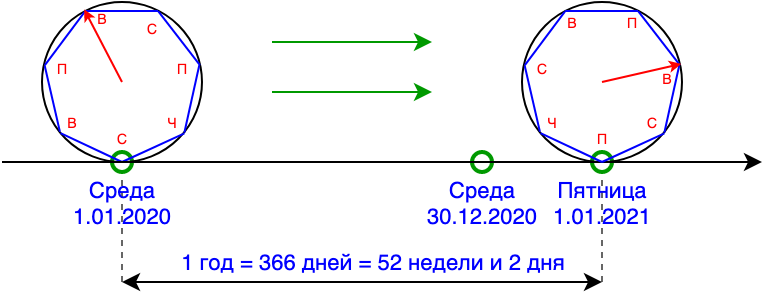
\includegraphics[scale=0.4]{weekdays.png}
\end{center}

\item Каждые 28 лет (а 28 --- это наименьшее общее кратное 7 и 4) соответствие дат и дней недели повторяется.
\item При расчетах на более длительные периоды, а именно, при переходе через 1900 год или 2100 год, нужно учитывать также, что 3 раза за 400 лет не происходит добавление лишнего дня (29 февраля) для более точного соответствия календаря астрономическому году, т.е. 1900, 1800, 1700 годы не являются високосными, как и 2100, 2200 и 2300.
\item Тем не менее, часто в жизни встречается задача вычисления дня недели, и здесь нам на помощь приходит исчисление остатков по модулю 7. Например, сегодня 21 марта 2020 суббота, а нам нужно знать, какой день недели будет 31 августа 2020. Сначала мы находим день недели 21 августа, т.к. до этой даты целое число месяцев. При этом мы 3 раза переходим через 31 число (март, май, июль) и 2 раза --- не переходим (апрель, июнь). Следовательно, 3 раза прибавляется остаток 3, и 2 раза --- остаток 2, итого сумма остатков составляет 13. Но это больше 7, причем очень близко к 14, поэтому сумму остатков мы запишем как -1. Наконец, остается добавить 10 дней (от 21 августа до 31 августа). Итого получается 9, а по модулю 7 --- всего 2. Таким образом, 31 августа 2020 года есть понедельник!
\item Из приведенной выше картинки с семиугольником на окружности, совмещенной с прямой линией, мы можем ясно представить себе, как работает исчисление остатков по модулю 7, т.е. исчисление дней недели. Мы катим окружность по прямой времени, пока не достигнем нужной нам даты. При этом неважно, сколько целых оборотов совершит семиугольник, т.е. сколько недель мы проедем, а вот последний полувиток как раз и дает нам ответ на вопрос о дне недели. Так что, если мы пронумеруем дни недели цифрами от 0 до 6, то любое расстояние между датами можно представить как какое-то целое количество недель плюс остаток, лежащие в диапазоне от 0 до 6 (включительно).
\item Эта картинка легко обобщается на случай произвольного основания. Представим, что в неделе у нас не 7 дней, а, например, 28 (лунный месяц), и тогда любое расстояние между датами выражается как целое число 28-дневных циклов плюс некоторый остаток от 0 до 27. И так далее.
\item Таким образом, мы приходим к тому, что всякое натуральное число (количество) можно представить в виде $a=km+b$, где $k$ --- неполное частное от деления $a$ на $m$, $b$ --- остаток от деления, который находится в промежутке от 0 (включая) до $m$ (не включая).
\item Равенство $a=km+b$ при исчислении остатков принято записывать так:
$$
a\equiv b\pmod m,
$$
Читается: $a$ сравнимо с $b$ по модулю $m$.

Причем, если модуль $m$ известен из контекста и не меняется при вычислениях, то его можно опускать, записывая просто $a\equiv b$. Читается: $a$ \textbf{сравнимо с} $b$ (по модулю $m$).

\item На картинке, приведенной выше, даты 1 января 2020 и 30 декабря 2020 сравнимы по модулю 7, т.е. по дням недели.
А про интервал в 366 дней мы запишем $366\equiv 2\pmod 7$. Такая запись никак не информирует нас о коэффициенте $k$ (количестве целых недель), но показывает самое главное --- сколько дней надо прибавить к среде.
\item Остатками можно оперировать так же, как обычными числами, сбрасывая всякий раз накопленные при сложении целые <<оброты>> модулей. Иначе говоря, если мы хотим, например, к текущей среде прибавить 6 дней, то мы совмещаем наш семиугольник вершиной <<среда>> с прямой времени, а затем прокатываем его вперед на 6 делений (что чуть меньше полного оборота), и в точке касания с прямой получаем вторник. Заметим, что ровно тот же результат мы получим, если прокатим семиугольник назад на 1 деление. Это значит, что числа 6 и -1 сравнимы по модулю 7. И на практике можно также пользоваться отрицательными числами для исчисления остатков.
\item Ранее мы много времени уделяли таблицам композиций движений многоугольников. И, как мы помним, композиция вращений многоугольника соответствовала сложению углов этих вращений. При этом мы также отбрасывали 360 градусов (или $2\pi$), если сумма углов переваливала за полный оборот. При описании конечных подгрупп движений правильных многоугольников мы выяснили, что каждый поворот является степенью некоторого минимального поворота на угол $2\pi/n$ (для $n$-угольника), т.е. все повороты выражаются углами $k(2\pi/n)$, где $k=0,\dots,n-1$ (ничего не напоминает?).
\item Забудем теперь про вращения и углы, а просто понаблюдаем за степенями этих поворотов при композициях, т.е. при сложении углов. Для примера рассмотрим случаи $n=7$ и $n=8$, и выпишем таблицу композиций, которая представлят собой таблицу сложения остатков по модулям 7 и 8, соответственно.
\item Таблицы сложения остатков по модулям 7 и 8:
\begin{center}
\begin{tabular}{c||c|c|c|c|c|c|c|}
  & 0 & 1 & 2 & 3 & 4 & 5 & 6 \\ \hline\hline
0 & 0 & 1 & 2 & 3 & 4 & 5 & 6 \\ \hline
1 & 1 & 2 & 3 & 4 & 5 & 6 & 0 \\ \hline
2 & 2 & 3 & 4 & 5 & 6 & 0 & 1 \\ \hline
3 & 3 & 4 & 5 & 6 & 0 & 1 & 2 \\ \hline
4 & 4 & 5 & 6 & 0 & 1 & 2 & 3 \\ \hline
5 & 5 & 6 & 0 & 1 & 2 & 3 & 4 \\ \hline
6 & 6 & 0 & 1 & 2 & 3 & 4 & 5 \\ \hline
\end{tabular}
\quad
\begin{tabular}{c||c|c|c|c|c|c|c|c|}
  & 0 & 1 & 2 & 3 & 4 & 5 & 6 & 7 \\ \hline\hline
0 & 0 & 1 & 2 & 3 & 4 & 5 & 6 & 7 \\ \hline
1 & 1 & 2 & 3 & 4 & 5 & 6 & 7 & 0 \\ \hline
2 & 2 & 3 & 4 & 5 & 6 & 7 & 0 & 1 \\ \hline
3 & 3 & 4 & 5 & 6 & 7 & 0 & 1 & 2 \\ \hline
4 & 4 & 5 & 6 & 7 & 0 & 1 & 2 & 3 \\ \hline
5 & 5 & 6 & 7 & 0 & 1 & 2 & 3 & 4 \\ \hline
6 & 6 & 7 & 0 & 1 & 2 & 3 & 4 & 5 \\ \hline
7 & 7 & 0 & 1 & 2 & 3 & 4 & 5 & 6 \\ \hline
\end{tabular}
\end{center}
Таблица сложения получается последовательными циклическими сдвигами верхней строки влево.


\item Помимо сложени остатков мы можем их умножать (в терминологии вращений многоугольника умножение соответствует многократной композиции одинаковых поворотов, так что первое число произведения отвечает за величину поворота, а второе --- за его кратность, либо наоборот).  Таблица умножения остатков по модулям 7 и 8 (отметим важную особенность этих таблиц: они имеют центральную симметрию, если вычеркнуть нулевые строку и столбец):
\begin{center}
\begin{tabular}{c||c||c|c|c|c|c|c|}
  & 0 & 1 & 2 & 3 & 4 & 5 & 6 \\ \hline\hline
0 & 0 & 0 & 0 & 0 & 0 & 0 & 0 \\ \hline\hline
1 & 0 & 1 & 2 & 3 & 4 & 5 & 6 \\ \hline
2 & 0 & 2 & 4 & 6 & 1 & 3 & 5 \\ \hline
3 & 0 & 3 & 6 & 2 & 5 & 1 & 4 \\ \hline
4 & 0 & 4 & 1 & 5 & 2 & 6 & 3 \\ \hline
5 & 0 & 5 & 3 & 1 & 6 & 4 & 2 \\ \hline
6 & 0 & 6 & 5 & 4 & 3 & 2 & 1 \\ \hline
\end{tabular}
\quad
\begin{tabular}{c||c||c|c|c|c|c|c|c|}
  & 0 & 1 & 2 & 3 & 4 & 5 & 6 & 7 \\ \hline\hline
0 & 0 & 0 & 0 & 0 & 0 & 0 & 0 & 0 \\ \hline\hline
1 & 0 & 1 & 2 & 3 & 4 & 5 & 6 & 7 \\ \hline
2 & 0 & 2 & 4 & 6 & 0 & 2 & 4 & 6 \\ \hline
3 & 0 & 3 & 6 & 1 & 4 & 7 & 2 & 5 \\ \hline
4 & 0 & 4 & 0 & 4 & 0 & 4 & 0 & 4 \\ \hline
5 & 0 & 5 & 2 & 7 & 4 & 1 & 6 & 3 \\ \hline
6 & 0 & 6 & 4 & 2 & 0 & 6 & 4 & 2 \\ \hline
7 & 0 & 7 & 6 & 5 & 4 & 3 & 2 & 1 \\ \hline
\end{tabular}
\end{center}
\item Отметим еще одно свойство таблицы умножения: строка или столбец, номер которого НЕ взаимно прост с модулем, содержит нули. Это легко доказать. Пусть номер строки равен $k$, и $s=\gcd(k,m)>1$. При этом ясно, что $s<m$, т.к. $s$ является делителем $m$. Пусть также $t=m/s$. Рассмотрим тогда строку $k$ и столбец $t$. Произведение их номеров равно $kt=km/s$. Поскольку $k/s$ также целое, получаем, что $kt$ кратно $m$, а значит, $kt\equiv 0\pmod m$. Отметим, что $s=1$ здесь не проходит ровно потому, что в этом случае $t$ не будет номером столбца таблицы умножения.
\item На самом деле, верно и обратное: если строка таблицы умножения содержит нули, то номер строки не взаимно прост с модулем. Для этого мы докажем эквивалентное утверждение
\begin{thrm}
Пусть $k>0$  и  $k\perp m$, тогда все остатки
$$
k,\quad 2k,\quad 3k,\quad\dots,\quad (m-1)k\pmod m
$$
попарно различны и отличны от нуля.
\end{thrm}
\pf Предположим, что один из остатков равен нулю: $kl\equiv 0\pmod m$, где $l\in\{1,2,\dots,m-1\}$. Тогда $kl=mt$ при некотором $t$. Но поскольку $k\perp m$, в силу ОТА число $k$ делит $t$, а значит, $k\le t$. Однако $l<m$, следовательно, $kl<mt$. Противоречие.

Далее, если среди остатков есть равные, например, $kl\equiv kt$, то здесь же найдется и остаток $k(l-t)$ (или $k(t-l)$, если $t>l$), который равен 0. А это невозможно по доказанному. 

Таким образом, эти остатки все различны и положительны, а значит, являются перестановкой множества $\{1,2,,\dots,m-1\}$.
\epf
\item Множество $\{0,1,2,\dots,m-1\}$ с операциями сложения и умножения по модулю $m$ называется \textbf{кольцом вычетов} по модулю $m$ и обозначается $\Z_m$.
\item Множество $\Z_m^*$, состоящее только из взаимно простых с модулем $m$ элементов $\Z_m$, образует группу по умножению остатков. Это легко увидеть из таблиц умножения, если исключить в них строки и столбцы, содержащие нули. Например, таблицей умножения для группы $\Z_8^*$ будет 
\begin{center}
\begin{tabular}{c||c|c|c|c|}
  & 1 & 3 & 5 & 7 \\ \hline\hline
1 & 1 & 3 & 5 & 7 \\ \hline
3 & 3 & 1 & 7 & 5 \\ \hline
5 & 5 & 7 & 1 & 3 \\ \hline
7 & 7 & 5 & 3 & 1 \\ \hline
\end{tabular}
\end{center}

\end{enumerate}



\subsection*{Задачи}
\begin{enumerate}
\item Если сегодня понедельник, от какой день недели будет через 10 дней, через 90 дней, через 2 года (невисокосных)?
\item Найти день недели через месяц, квартал, полгода и год, отправляясь от текущей даты.
\item Построить таблицы сложения и умножения для остатков: 2,3,4,5,6.
\item Сравнить таблицу сложения остатков по модулю 2 с таблицами умножения классов сдвигов $\T$ и симметрий $\S$ для прямой и окружности.
\item Сравнить таблицу симметрий ромба с таблицей умножения группы $\Z_8^*$.
\item В группе $\Z_8^*$ найти обратные элементы: $3^{-1}, 5^{-1}, 7^{-1}$.
\item Проверить, что $\Z_m$ удовлетворяет аксиомам кольца.
\end{enumerate}

\section{Свойства арифметики остатков}
\subsection*{Конспект}
\begin{enumerate}
\item Свойства сравнений таковы:
\begin{enumerate}[M1.]
\item $a\equiv b\pmod m$ тогда и только тогда, когда $a-b$ кратно $m$;
\item если $a\equiv b$, $c\equiv d$, то $a+c\equiv b+d$, $a-c\equiv b-d$ и $ac\equiv bd$;
\item для $n\ge 0$ если $a\equiv b$, то $a^n\equiv b^n$;
\item признаки делимости на $3$ и на $9$: $a_0+a_110+a_210^2+\dots+a_n10^n\equiv a_0+\dots+a_n$ по модулю $3$ и по модулю $9$;
\item если $m>0$ и $d\perp m$, то
$$
ad\equiv bd\pmod m\iif a\equiv b\pmod m
$$
\item  если $m,d>0$, то
$$
ad\equiv bd\pmod{md}\iif a\equiv b\pmod m
$$
\item  если $m>0$, то для любого $d$
$$
ad\equiv bd\pmod m\iif a\equiv b\pmod{m/\gcd(m,d)}
$$
\item  если $m,d>0$, $a\equiv b\pmod{md}$, то $a\equiv b\pmod{m}$
\item если $m,n>0$, то
$$
a\equiv b\pmod m,\quad a\equiv b\pmod n\iif a\equiv b\pmod{\nok(m,n)}
$$
\item если $m,n>0$ и $m\perp n$, то
$$
a\equiv b\pmod m,\quad a\equiv b\pmod n\iif a\equiv b\pmod{mn}
$$
\item пусть $n_p$ --- степень простого числа $p$ в разложении $n$ по степеням простых (ОТА), тогда
$$
a\equiv b\pmod n\iif \forall p\quad a\equiv b\pmod{p^{n_p}}\quad\textup{($p$ --- простое)}
$$
\end{enumerate}
\item \textbf{Китайская теорема об остатках}.
Пусть числа $m_1,\dots,m_k>0$ попарно взаимно просты, $m=m_1\dots m_k$. Тогда
$$
a\equiv b\pmod m\iif a\equiv b\pmod{m_j},\quad j=1,\dots,k
$$
\item \textbf{Малая теорема Ферма}: $n^{p-1}\equiv 1\pmod p$, где $p$ --- простое и $p\not| m$.
\item Малая теорема Ферма обеспечивает существование обратных элементов в группе по умножени остатков $\Z_p^*$. Достаточно $n$ умножить на $n^{p-2}$, и мы получим 1.
\item Отсюда следует, что $\Z_p$ при простом $p$ является \textbf{полем}.
\item Поле --- это кольцо, в котором все ненулевые элементы обратимы. Кольцо целых чисел не является полем. Рассмотренные нами ранее группы движений также нельзя назвать полем, т.к. в них всего одно операция. Первое поле, которое мы встречаем в курсе --- это $\Z_p$, поле вычетов по простому модулю.
\end{enumerate}
\subsection*{Задачи}

\begin{enumerate}
\item Доказать, что $2^n-1$ кратно трем тогда и только тогда, когда $n$ --- четное, и $2^n+1$ кратно трем тогда и только тогда, когда $n$ --- нечетное.
\item Что означает запись $a\equiv b\pmod 0$?
\item В силу ОТА будем записывать положительное натуральное число $m$ как последовательность $\bar m$ степеней простых:
$$
m=p_0^{\al_0}p_1^{\al_1}\dots p_k^{\al_k}\ldots\iff \bar m=(\al_0,\al_1,\dots,\al_k,\dots),
$$
где $p_0<p_1<p_2<\dots$ --- все простые числа, начиная с 2.

Докажите, что если $\bar m=(\al_0,\al_1,\dots,\al_k,\dots)$ и $\bar n=(\be_0,\be_1,\dots,\be_k,\dots)$, то
\begin{align*}
\bar{nm} = & (\al_0+\be_0,\al_1+\be_1,\dots,\al_k+\be_k,\dots) \\
\bar{\gcd(n,m)} = & (\min(\al_0,\be_0),\min(\al_1,\be_1),\dots,\min(\al_k,\be_k),\dots), \\
\bar{\nok(n,m)} = & (\max(\al_0,\be_0),\max(\al_1,\be_1),\dots,\max(\al_k,\be_k),\dots).
\end{align*}

\item Докажите, что $\gcd(n,m)\nok(n,m)=nm$.
\item Докажите, что
$$
\gcd(kn,km)=k\gcd(n,m),\quad \nok(kn,km)=k\nok(n,m).
$$
\end{enumerate}



\section{*Вычеты и операции Минковского}

\vrezka{Данный раздел нужно изучать вместе с главой 0. При первом чтении можно пропустить.}

\subsection*{Конспект}
\begin{enumerate}
\item Вернемся к арифметическим операциям над множествами. Пусть задано целое число $m>1$, тогда
$$
m\Z = \{mk\mid k\in Z\}.
$$
\item Как мы помним, это --- кольцо, т.е. в $m\Z$ можно складывать, вычитать и умножать, но нельзя делить любое число на любое ненулевое. Что будет если сдвинуть его на некоторое целое число? Т.е. взять множество
$$
m\Z+n = \{mk+n\mid k\in\Z\}
$$
\item При каких $n$ множество $m\Z+n$ останется кольцом? В кольце должен быть ноль, следовательно, если $m\Z+n$ --- кольцо, то при некотором $k$ имеем $mk+n=0$, откуда следует, что $n$ кратно $m$. Обратно, если $n$ кратно $m$, то $m\Z+n=m\Z$. Действительно, $n=km$, и тогда $ml+n=m(l+k)\in m\Z$, т.е. $m\Z+n\subseteq m\Z$. Кроме того, $ml=m(l-k)+mk=m(l-k)+n$, откуда $m\Z\subseteq m\Z+n$. Таким образом, $m\Z+n=m\Z$.
\item Итак, $m\Z+n$ остается кольцом тогда итолько тогда, когда $n$ кратно $m$, причем это все то же кольцо $m\Z$.
\item Пусть теперь $n=mk+d$, где $d$ --- остаток от деления $n$ на $m$.
\item В этом случае $m\Z+n=m\Z+mk+d=m\Z+d$. Отсюда легко получить следующее совйство
$$
m\Z+n = m\Z+n' \iff n\equiv n' \pmod m,
$$
т.е. сложение с $m\Z$ в каком-то смысле напоминает операцию сложения по модулю $m$ --- оно <<забывает>> все, что кратно $m$, оставляя только остаток.
\item Это значит, что существует ровно $m$ различных множеств вида $m\Z+n$, а именно:
$$
m\Z,\quad m\Z+1,\quad\dots,\quad m\Z+m-1.
$$
\item Далее, эти множества попарно не пересекаются и в сумме дают все $\Z$. Это утверждение предлагается доказать самостоятельно.
\item \textbf{Важный логический шаг!} Рассмотрим теперь множества $m\Z+n$ как новые элементы (т.е. мы забываем их природу и считаем их отдельными точками, такими же, как до этого считали целые числа) и соберем из них новое множество
$$
\Z/m\Z = \{m\Z,\quad m\Z+1,\quad\dots,\quad m\Z+m-1\},
$$
которое в алгебре называется \textbf{фактормножеством}.
\item Наконец, вспомним о том, что мы можем умножать и складывать множества, т.е. определны операции Минковского
$$
(m\Z+n)+(m\Z+n'),\quad (m\Z+n)(m\Z+n').
$$
\item Нетрудно показать следующие свойства этих операций:
\begin{enumerate}[Z1]
\item $(m\Z+n)+(m\Z+n') = m\Z+(n+n'\mod m)$
\item $(m\Z+n)(m\Z+n') = m\Z+(nn'\mod m)$
\end{enumerate}
Действительно, $mk+n+mk'+n'\equiv n+n'\pmod m$ и $(mk+n)(mk'+n')\equiv nn'\pmod m$.
\item Это значит, что операции Минковского над элементами $\Z/m\Z$ в точности дают алгебру остатков, которую мы рассматривали выше.
\item То есть $\Z/m\Z$ --- кольцо, построенное на фактормножестве, причем его операциями являются операйии Минковского, определенные через операции исходного кольца. Такое кольцо назвается \textbf{факторкольцом} кольца $\Z$.
\item \textbf{Зафиксируем}: в исходном кольце (например, $\Z$) рассматривается подкольцо (например, $m\Z$) и все его сдвиги, полученные смещением на элементы этого же кольца, получается набор множеств, попарно не пересекающихся и дающих в сумме исходное кольцо, далее на этих множествах вводятся операции сложения и умножения, полученные как операции Минковского. Итоговая стрктура называется факторкольцом.
\item Аналогично можно построить такое понятие как факторгруппа, воспользовавшись лишь одной операцией --- сложением.
\item Факторкольца и факторгруппы являются мощным инструментом абстракции и получения общих результатов в алгебре и теории множеств.
\end{enumerate}


\subsection*{Задачи}
\begin{enumerate}
\item Доказать, что $m\Z+n\cap m\Z+n'=\emptyset$, если $0\le n<n'\le m-1$.
\item Доказать, что
$$
m\Z\cup (m\Z+1)\cup\dots\cup (m\Z+m-1) = \Z.
$$
\item Построить факторкольцо $(\Z/6\Z)/2(\Z/6\Z)$. Алгебру остатков по какому модулю мы получим?
\item Построить факторкольцо $(\Z/6\Z)/5(\Z/6\Z)$. Почему получается одноэлементное фактормножество, т.е. тривиальное кольцо, состоящее из одного нуля.
\end{enumerate}


\section{*Теория множеств: отношения}\label{Rels}

\vrezka{Данный раздел нужно изучать вместе с главой 0. При первом чтении можно пропустить.}


\subsection*{Конспект}
\begin{enumerate}
\item Пусть заданы два множетва $A$ и $B$. Под их \textbf{прямым произведением} мы понимаем множество всех пар точек $(a,b)$, где $a\in A$, $b\in B$. Пары при этом обладают свойством позиционного равенства, т.е.
$$
(a,b)=(c,d) \iff (a=c)\land (b=d)
$$
\item Обозначение для прямого произведения:
$$
A\times B = \{(a,b)\mid a\in A, b\in B\}.
$$
\item В качестве примера можно рассмотреть множество пар целых чисел на плоскости или, например, таблицу умножения остатков, где помимо пары чисел еще задано значение их произведения по модулю.
\item \textbf{Отношением между множествами} $A$ и $B$ называется всякое подмножество $R\subseteq A\times B$. Обычно вместо $(a,b)\in R$ принято записывать $aRb$. В случае, когда $A=B$, говорят, что $R$ есть отношение \textbf{на множестве} $A$
\item Примеры отношений:
\begin{enumerate}[R1]
\item Отношение отец--сын ($a$ есть отец $b$). Оно \textit{несимметричное}!
\item Отношение предок--потомок. Оно также несимметричное, но \textit{транзитивное}! Если $a$ есть предок $b$ и $b$ есть предок $c$, то $a$ есть предок $c$.
\item Отношение братства: $a$ есть брат $b$. Оно и симметричное, и транзитивное (имеются ввиду родные братья, т.е. у них общий отец).
\item Отношение $a<b$ на целых числах: транзитивное и \textit{антисимметричное}: невозможно одновременно $a<b$ и $b<c$
\item Отношение сравнения по модулю: $a\equiv b\pmod m$. Это отношение симметрично, транзитивно и \textit{рефлексивно}, т.е. всякое число само с собой сравнимо.
\end{enumerate}
\item Если отношение симметрично, рефлексивно и транзитивно, то оно называется \textbf{отношением эквивалентности}.
\item Отношение сравнения по модулю --- отношение эквивалетности.
\item Обычное равенство --- отношение эквивалетности.
\item Если каждого человека считать братом самому себе, то отношение братства становится отношением эквивалентности.
\item Отношение эквивалентности разбивает множество, на котором оно задано, на неперсекающиеся классы эквивалентности:
$$
A = A_1\sqcup A_2\sqcup\dots
$$
При этом внутри каждого класса сидят эквивалентные друг другу элементы. Например, всех мужчин можно разделить на классы эквивалентности, в каждом из которых находятся родные братья.
\item А еще можно рассмотреть классы эквивалентности по отношению сравнимости целых чисел по заданному модулю. И этими классами будут:
$$
m\Z,\quad m\Z+1,\quad m\Z+2,\quad\dots,\quad m\Z+m-1
$$
Именно эти классы у нас формировали фактормножетво $\Z/m\Z$!
\item Вообще, если $R$ есть отношение эквивалентности на множестве $A$, то множество классов эквивалентности обозначается $A/R$ и называется фактормножеством множества $A$ по отношению эквивалентности $R$.
\end{enumerate}


\subsection*{Задачи}
\begin{enumerate}
\item Чему равно $\emptyset\times\emptyset$, $A\times\emptyset$, $\emptyset\times B$?
\item Найти $\{1,2,3\}\times\{\emptyset\}$.
\item В чем отличие $\{a,b\}\times\{1,2\}$ от $\{1,2\}\times\{a,b\}$?
\item Постройте фактормножество множества $\Z_9$ по отношению сравнимости по модулю $3$.
\item Рассмотрим группу движений правильного $n$-угольника. Пусть два движения эквивалентны, если их композиция является поворотом (или $\id$). Докажите, что это и в самом деле отношение эквивалентности, постройте классы эквивалентности, постройте факторгруппу на этих классах. Какова ее таблица умножения?
\item **Изучить картинки с примерами отношений, почему они так выглядят? Функция $\lfloor x\rfloor$ обозначает целую часть числа. Здесь мы неявно предполагаем знакомство продвинутого читателя с нецелыми числами.
\end{enumerate}
\begin{center}
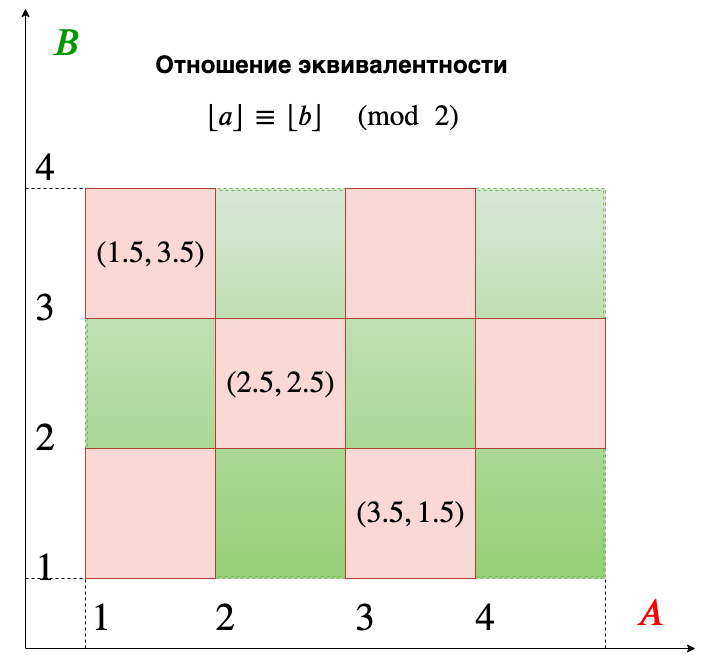
\includegraphics[scale=0.25]{equiv.png}
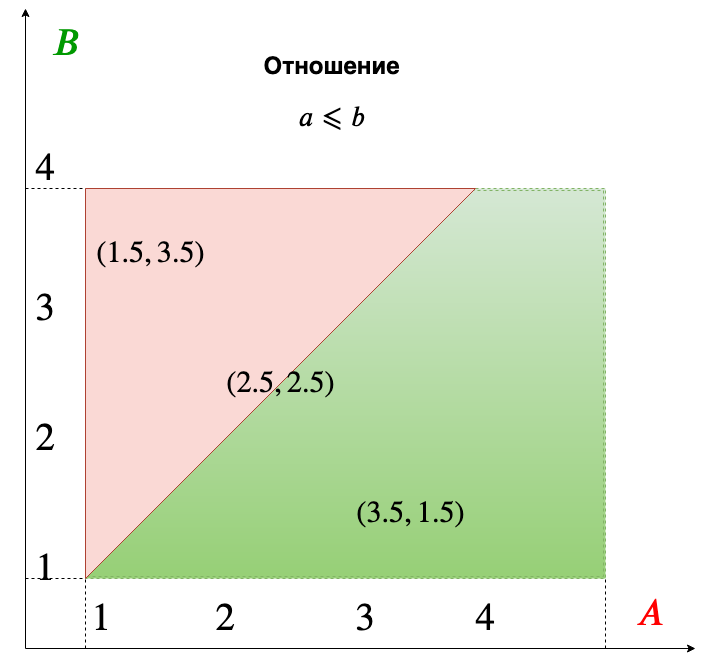
\includegraphics[scale=0.25]{lessthan.png}
\end{center}





\chapter{Движения плоскости и пространства}

\vrezka{Данная глава продолжает тему групп движений. Здесь мы получаем теорему Шаля (для движений плоскости), а затем широкими мазками освещаем тему движений сферы и пространства. 

Разделы о сфере и пространстве могут быть пропущены при первом ознакомлении с конспектом.
}

\section{Виды движений плоскости. Теорема Шаля}

\subsection*{Конспект}
\begin{enumerate}\setlength{\itemsep}{1pt}
\item Разбираем движения, попутно доказывая лемму <<о гвоздях>>.
\item Пусть на плоскости три точки, не лежащие на одной прямой, остаются неподвижными при движении. Вывод: это $\id$.
\item Пусть на плоскости неподвижны 2 точки и вся прямая, проходящая через них, остальные точки подвижны. Тогда это симметрия относительно данной прямой.
\item Пусть неподвижна лишь одна точка. Такое возможно лишь при вращении вокруг этой точки на угол, не кратный полному обороту.
\item Пусть вообще нет неподвижных точек. Берем любую точку, смотрим, куда она переходит, применяем сдвиг (параллельный перенос). Оставшееся преобразование имеет как минимум 1 неподвижную точку, а значит, является либо $\id$, либо симметрией, либо поворотом. Интересно, что поворот в данном случае можно исключить, т.к. композиция сдвига и поворота есть просто поворот, а значит, в исходном преобразовании была как минимум одна неподвижная точка. Следовательно, исходное движение есть либо сдвиг, либо смещенная симметрия (композиция сдвига и симметрии).
\item Таким образом, движение плоскости можно рассматривать как комбинацию параллельного переноса (в частности, на нулевой вектор), поворота (в частности, на нулевой угол) и симметрии относительно произвольной прямой.
\item \textbf{Теорема Шаля}. Произвольное движение (без разложения его на компоненты) есть движение одного из следующих классов:
\begin{enumerate}[a)]
\item класс параллельных переносов (на произвольный вектор), который мы обозначим $\rightrightarrows$;
\item класс поворотов относительно произвольного центра, который мы обозначим $\circlearrowleft$;
\item класс \textbf{скользящих симметрий} (сдвиг на произвольный вектор с последующей симметрией относительно оси данного вектора), который мы обозначим $\leftharpoonup\leftharpoondown$.
\end{enumerate}
\item Таблица композиций для таких классов выглядит следующим образом:
\begin{center}
\begin{tabular}{c|ccc}
 & $\rightrightarrows$ & $\circlearrowleft$ &  $\leftharpoonup\leftharpoondown$ \\ \hline
$\rightrightarrows$ & $\rightrightarrows$ &  $\circlearrowleft$ &  $\leftharpoonup\leftharpoondown$  \\ 
$\circlearrowleft$ & $\circlearrowleft$ & $\rightrightarrows$ или $\circlearrowleft$ & $\leftharpoonup\leftharpoondown$  \\ 
$\leftharpoonup\leftharpoondown$ & $\leftharpoonup\leftharpoondown$ & $\leftharpoonup\leftharpoondown$ & $\rightrightarrows$ или $\circlearrowleft$  \\ 
\end{tabular}
\end{center}
\item Аналогично одномерным случаям (прямая и окружность) можно выбирать различные базовые преобразования для построения с их помощью всех движений. 
\item Всякое движение есть композиция не более трех симметрий (относительно разных и, вообще говоря, не обязательно параллельных осей).
\item Сдвиг можно представить как композицию двух симметрий (относительно параллельных осей).
\item Поворот можно представить как композицию двух симметрий (относительно пересекающихся осей).
\item Скользящую симметрию можно представить как композицию трех симметрий (две на сдвиг и одна собственно симметрия).
\end{enumerate}


\subsection*{Задачи}
\begin{enumerate}
\item Показать, что композиция поворотов (относительно разных центров) есть либо сдвиг, либо поворот (вычислить его центр).
\item Показать, что композиция сдвига и поворота есть поворот.
\end{enumerate}


\section{Сравнение движений прямой, окружности и плоскости}
\subsection*{Конспект}
\begin{enumerate}
\item Отметим несколько общих свойств рассмотренных нами движений прямой, окружности и плоскости.
\item Во-первых, их всех можно свести к композиции симметрий. Для одномерных объектов (прямая и окружность) --- не более двух, для двумерных --- не более трех.
\item Во-вторых, все движения можно разделить на два класса: сохраняющие и меняющие \textbf{ориентацию}. Те движения, которые сводятся к композиции четного числа симметрий, сохраняют ориентацию фигур, а те, которые сводятся к композиции нечетного числа симметрий, --- меняют ориентацию фигур. Изменение ориентации означает, что право и лево меняются местами, т.е. мы как бы переходим в зазеркалье. 
\item При этом нужно отметить, что преобразования, меняющие ориентацию, обязательно требуют выхода в пространство, если мы хотим осуществить их непрерывным движением.
\item В-третьих, есть и более глубинная связь движений прямой, окружности и плоскости. Мы уже отмечали, что окружность можно рассматривать как прямую, у которой склеили противоположные концы (где-то на бесконечности). И с этой точки зрения сдвиг на прямой является прямой аналогией вращения окружности. Особенно, если величина сдвига сильно меньше радиуса.
\item А симметрия прямой при этом естественным образом превращается в симметрию окружности. Только ось симметрии должна проходить через место склейки двух бесконечностей. Остальные же симметрии можно получить дополнительным сдвигом, т.е. вращением.
\item Далее, окружность находится на плоскости. И поэтому вращение окружности полностью аналогично вращению плоскости, если при этом совместить их центры.
\item Еще проще увидеть совпадения понятий сдвига на прямой и плоскости. В обоих случаях мы просто смещаем все точки на какой-то вектор.
\item Тем не менее, на плоскости появляется новый вид движения, который комбинирует в себе сдвиг и отражение относительно оси сдвига. Это --- скользаящая симметрия, т.е. симметрия с последующим применением сдвига вдоль оси симметрии. На одномерных объектах такое движение в принципе невозможно. На прямой симметрия относительно этой же прямой ничего не дает, т.е. является $\id$, а на окружности симметрия относительно самой окружности вообще требует специального построения в геометрии плоскости.
\end{enumerate}


\section{Векторно-числовое представление движений плоскости}

\subsection*{Конспект}

\begin{enumerate}
\item \textbf{Аффинное пространство} --- множество точек и векторов. В аффинном пространстве мы работаем сразу с двумя сортами объектов --- точками и векторами, на которых заданы операции сложения и вычитания. При этом в сумме $a+b$ и разности $a-b$ могут быть такие комбинации:
\begin{enumerate}[1)]
\item $a$ --- точка, $b$ --- вектор, результатом $a+b$ будет точка, соответствующая концу вектора $b$, когда он отложен от точки $a$, результатом $a-b$ будет точка $c$ такая, что $c+b=a$;
\item $a$ и $b$ --- векторы, результатом $a+b$ будет вектор, построенный по правилу параллелограмма, результатом $a-b$ будет вектор $c$ такой, что $c+b=a$;
\item $a$ и $b$ --- точки, результатом $a-b$ будет вектор с началом в точке $b$ и концом в точке $a$.
\end{enumerate}
\item Движения --- это преобразования точек. Параметром движения может быть вектор и/или угол (число).
\item Сдвиг на плоскости на вектор $a$ обозначим $T_a$. Операция $T_a$ осуществляет прибавление вектора $a$ к точкам плоскости. Композиция сдвигов соответствует сумме векторов сдвига: $T_a\circ T_b=T_{b+a}$.
\item Поворот вокруг нуля мы ранее обозначали $R_\al$, где $\al$ --- угол в радианах.
\item Поворот на угол $\al$ относительно произвольной точки $M$ можно выразить так:
$$
R_{M,\al} = T_{O+M}\circ R_\al\circ T_{O-M},
$$
т.е. сначала сдвигаем точку $M$ в центр вращения, отмеченный точкой $O$, затем производим вращение, затем возвращаем точку $M$ на место обратным сдвигом.
\item Наконец, у нас остается такой вид движения, который осуществляет отражение относительно произвольной прямой на плоскости. Обозначим его $S_l$.
\item Предположим, что на плоскости помимо точки $O$ мы также зафиксировали некоторую прямую, проходящую через $O$ с выделенным направлением $OA$ ($A$ лежит на этой прямой и не совпадает с $O$). Зафиксируем отражение $S_{OA}$ относительно данной выбранной оси $OA$. Отметим, что $S_{OA}=S_{AO}$, т.е. отражение не зависит от направления оси отражения.
\item Выразим произвольное отражение через базовое отражение $S_{OA}$ и другие движения. Для этого обозначим через $M$  произвольную точку прямой $l$, через $\al$ --- угол наклона прямой $l$ относительно направления $OA$. Тогда
$$
S_l = T_{O+M}\circ R_\al \circ S_{OA} \circ R_{-\al}\circ T_{O-M},
$$
т.е. сначала мы сдвигаем плоскость так, чтобы точка $M$ оказалась в точке $O$, затем выполняем поворот на угол $-\al$, далее выполняем стандартное отражение, а затем производим обратные операции, которые возвращают прямую $l$ на место.
\item Соответственно, скользящая симметрия, при которой выполняется отражение относительно оси $l$ и сдвиг на вектор $MM'$ ($M,M'\in l$), записывается так:
$$
S_l = T_{O+M}\circ R_\al \circ S_{OA} \circ R_{-\al}\circ T_{O-M}\circ T_{M'-M},
$$
\item В терминах движений $T,R,S$ можно записать все возможные виды движений плоскости, т.е. сдвиг на произвольный вектор, поворот на произвольный угол относительно произвоьлной точки, скользящую симметрию относительно произвольной прямой $l$ со сдвигом на произвольный вектор, лежащий на этой прямой.
\item Если мы вернемся на окружность, то нам потребуется исключить сдвиги, оставив только вращения и симметрии.
\end{enumerate}




\section{Пара слов о движениях сферы}
\subsection*{Конспект}
\begin{enumerate}
\item Имея опыт перехода от прямой к окружности, мы можем легко найти движения сферы, отправляясь от движений плоскости.
\item Представим себе сферу как плоскость, у которой бесконечно удаленный край был стянут в точку (метод <<хинкали>>).
\item Во что превращаются при этом движения плоскости?
\item Сдвиг, он же параллельный перенос, превращается в такое движение, при котором все точки движутся по параллельным траекториям. С точки зрения географии это есть движение вдоль широтных линий. Да, проходят они при этом разное расстояние! Из-за чего, кстати, и появляются силы Кориолиса, создающие океанические течения вроде Гольфстрима. Но собственные расстояния между точками сохраняются, и это, несомненно, движение.
\item Вращение, которое, как мы помним, на окружности соответствует сдвигу на прямой, в случае сферы в прямом смысле слова совпадает со сдвигом! Дело в том, что вращение сферы вокруг оси, --- это вращение вокруг полюса, при котором угол поворота измеряется меридианом. Но ведь то же самое движение около экватора есть то, что мы только что отнесли к сдвигам вдоль широтных линий.
\item Таким образом, сдвиг прямой и вращение окружности в случае сферы чудесным образом объединяются в один вид движений --- осевое вращение. И это делает движения сферы чуть проще, чем движения плоскости, где сдвиг можно представить лишь как композицию двух вращений.
\item Далее, симметрия плоскости относительно прямой естественным образом переходит в отражение сферы относительно центральной секущей плоскости или, иначе говоря, относительно окружности большого круга. При такой симметрии полюса сферы меняются местами (полюса определются пересечением со сферой прямой, пересекающей плоскость отражения в центре сферы и перпендикулярной ей), а плоскость отражения остается на месте.
\item Наконец, скользящая симметрия плоскости есть композиция сдвига и осевой симметрии, и ей на сфере соответствует \textbf{зеркальное вращение}, т.е. композиция отражения и вращения параллельно плоскости отражения.
\item Таким образом, все движения сферы распадаются на два класса: вращения и зеркальные вращения. При этом, все движения есть композиция не более чем трех отражений.
\item Этот аналог теоремы Шаля для сферы можно доказать, используя очередную лемму о гвоздях, предполагая неподвижность пары противоположых точек (случай одной точки на плоскости), неподвижность целой окружности большого круга (случай двух точек на плоскости), отсутствие неподвижных точек.
\end{enumerate}

\subsection*{Задачи}
\begin{enumerate}
\item Построить таблицу движений сферы аналогично таблице движений плоскости (символику придумайте сами).
\item **Доказать, что других движений на сфере не существует (лемма о гвоздях).
\end{enumerate}


\section{Пара слов о движениях пространства}
\subsection*{Конспект}
\begin{enumerate}
\item Наконец, мы можем от сферы перейти к пространству. На самом деле, переход в пространство сопровождается лишь добавлением сдвига в пространстве. Т.е. любое движение сферы можно рассматривать как движение пространства с одной неподвижной точкой --- центром сферы. После чего можно применить сдвиг этого центра, и получить новые движения. Понятно, что никаких других движений тут быть не может.
\item Тем не менее, классификация движений пространства становится сложнее примерно так же, как классификация движений плоскости превосходит классификацию движений окружности. А именно, в пространстве появляется \textbf{винтовое движение} как композиция осевого вращения и сдвига вдоль оси вращения. Это --- обобщение скользящей симметрии на плоскости (если винт осуществляет поворот на $180^0$, мы как раз получаем скользящую симметрию).
\item Есть также и собственно \textbf{скользящая симметрия пространства}. Это --- отражение относительно плоскости с последующим сдвигом вдоль направления, параллельного данной плоскости. Такое движение также является обобщением скользящей симметрии на плоскости.
\item Заметим, что более сложное движение винт включает в себя более простые. Так, если винт имеет нулевой сдвиг, то он доставляет осевое вращение, а если винт имеет нулевой поворот, то он доставляет сдвиг. Понятно, что в случае полного зануления параметров винта мы получим $\id$.
\item Точно так же, \textbf{зеркальное вращение}, как и в случае сферы, при нулевом повороте доставляет просто симметрию.
\item Наконец, скользящая симметрия своим частным случаем имеет просто симметрию относительно плоскости.
\item Таким образом, классификация движений пространства включает следующие виды движений:
\begin{enumerate}[a)]
\item винт (в частности, сдвиг, осевое вращение, $\id$);
\item зеркальное вращение (в частности, отражение);
\item скользящая симметрия (в частности, отражение).
\end{enumerate}
\end{enumerate}

\subsection*{Задачи}
\begin{enumerate}
\item Построить таблицу движений пространства аналогично таблице движений плоскости (символику придумайте сами).
\item *Показать, что центральная симметрия пространства --- это зеркальное вращение.
\item **Доказать, что других движений в пространстве не существует (лемма о гвоздях).
\end{enumerate}


\begin{sidewaystable}
\caption{Сравнение движений.}
\label{Transitions}
\begin{tabular}{p{2cm}|p{2.5cm}p{2.5cm}p{2.5cm}p{2cm}p{2.5cm}p{2.5cm}}
\rowcolor{darkred}
& \multicolumn{3}{P{8.5cm}}{\textcolor{white}{\bfseries Собственные движения\linebreak (не меняют ориентацию)}} & \multicolumn{3}{P{8cm}}{\textcolor{white}{\bfseries Несобственные движения\linebreak (меняют ориентацию)}} \\ 
& Перенос & Поворот & Смещение поворота & Симметрия & \multicolumn{2}{p{5cm}}{Смещенная симметрия} \\ \hline \hline
Прямая     & сдвиг на число & & & относи\-тель\-но точки & & \\  \hline
Окруж\-ность & \multicolumn{2}{p{5cm}}{\centerline{вращение}} & & осевая симметрия & & \\ \hline
Плос\-кость  & параллель\-ный перенос & относи\-тель\-но точки & & осевая симметрия & скользящая симметрия (перенос+ сим\-мет\-рия) & \\  \hline
Сфера & вращение вблизи экватора & вращение вблизи полюса & & отражение относительно плоскости & \multicolumn{2}{p{5cm}}{зеркальное вращение (вращение+симметрия)} \\ \hline
Прост\-ранство & параллель\-ный перенос & осевое вращение & винт (перенос + вращение) & отражение относительно плоскости & скользящая симметрия (перенос+ сим\-мет\-рия) & зеркальное вращение (вращение+ сим\-мет\-рия) \\ \hline \hline
\end{tabular}
\end{sidewaystable}















\chapter{Линейные уравнения}

\vrezka{
Основная задача данной главы --- дать полное описание решений линейных уравнений в целях числах. Попутно вводится уравнение прямой на координатной плоскости, хотя мы все еще подразумеаем, что работаем только с целыми числами.
}

\section{Уравнение прямой на плоскости}

\subsection*{Конспект}

\begin{enumerate}
\item Рассмотрим плоскость с координатными осями $Ox$ и $Oy$. Что будет, если ее начать поворачивать? Во что переходит при этом ось $Ox$?
\item Поскольку вращение --- это движение, расстояние между точками сохраняется, и значит, никакие три точки, лежащие на прямой $Ox$, при повороте не могут перейти в точки, образующие невырожденный треугольник --- они снова лягут на прямую, причем в том же самом порядке. Стало быть, $Ox$ при вращении плоскости переходит в некоторую прямую.
\item Пусть центорм вращения является точка $O=(0,1)$, и ось $Ox$ при вращении $R_\ph$ переходит в прямую $l$. Ясно, что $l$ такаже проходит через начало координат $O$, т.к. это --- стационарная точка вращения.
\item Фиксируем на $Ox$ точку $(1,0)$ и посмотрим, куда она переходит под действием всех возможных вращений. Поскольку расстояние от центра вращения сохраняется, ясно, что эта точка остается на окружности радиуса 1. В то же время, выбирая произвольную точку на этой окружности, мы легко укажем угол $\ph$, на который нужно осуществить поворот плоскости относительно центра $O$, чтобы точка $(1,0)$ перешла в выбранную нами точку.
\item Итак, под действием группы вращений точка $(1,0)$ переходит во все точки единичной окружности. Аналогично, если мы выберем произвольную точку $(r,0)$ ($r>0$), она будет переходить во все точки окружности радиуса $r$ под действием группы вращений с центром в точке $O$.
\item В этом случае принято говорить, что группа вращений \textbf{действует} на плоскости, а множество всех значений, в которые она переводит выбранную точку, называют \textbf{орбитой} этой точки. В нашем примере орбитами являются коцентрические окружности с центром $O$.
\item Можно доказать, что орбиты образуют классы экивалентности, т.е. они попарно не пересекаются и в сумме дают всю область действия группы.
\item Фиксируем некоторое вращение $R_\ph$, и пусть точка $(0,1)$ при таком вращении перешла в точку $C=(x_0,y_0)$, лежащую на единичной окружности.
\item Возьмем произвольную точку $(r,0)$, где $r>0$, и проследим ее судьбу под действием того же вращения $R_\ph$. Пусть $A=(x,y)=R_\ph(r,0)$. Ясно, что точки $O,C,A$ лежат на одной прямой $l$.
\item Проведем вертикальные линии через абсциссы $x_0$ и $x$, а также горизонтальные линии через ординаты $y_0$ и $y$. Добавим новые точки пересечения $B$ и $D$ (см. рисунок).

\begin{center}
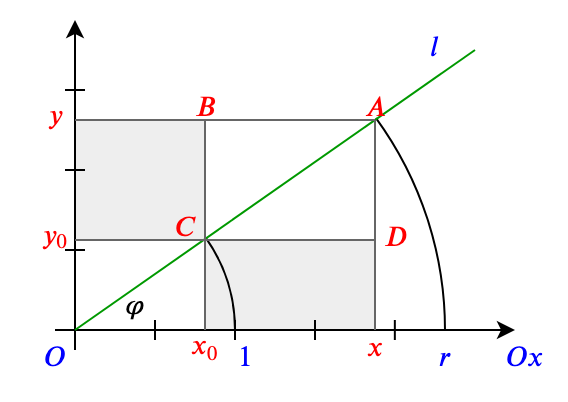
\includegraphics[scale=0.5]{linerotation.png}
\end{center}
\item Видим, что треугольники $ABC$ и $ADC$ равны по трем сторонам, также равны треугольники $Oy_0C$ и $Ox_0C$, и треугольники $OyA$ и $OxA$. Отсюда легко установить равенство площадей $x_0(y-y_0)=y_0(x-x_0)$, откуда получаем
$$
xy_0-yx_0=0.
$$
\item Поскольку $(x,y)$ --- это произвольная точка прямой $OC$ (для отрицательного $r$ все доказывается аналогично),  данное уравнение есть уравнение прямой, проходящей через начало координант с углом наклона $\ph$.
\item Отметим, что точка $(x_0,y_0)$ полностью определяется углом поворота $\ph$, т.к. является образом точки $(0,1)$ при повороте на угол $\ph$. В то же время, произвольная точка на единичной окружности однозначно задает угол поворота в интервале от 0 до $2\pi$. Таким образом, задать поворот с центром $O$ и задать точку на единичной окружности --- суть одно и то же.
\item Зная тригонометрию, можно также заметить, что $x_0=\cos\ph$ и $y_0=\sin\ph$, а отношение $y_0/x_0=\tan\ph$.
\item Кроме того, отношение $y_0/x_0$ также однозначно определяет угол поворота, но только в интервале от 0 до $\pi$.
\item Наконец, поворот прямой(!) на угол $\pi+\al$ --- это поворот на угол $\al$ с последующим отражением прямой $l$ относительно точки $O$. Но отражение прямой относительно своей же точки дает нам ту же самую прямую с тем же самым уравнением для ее точек! Таким образом, прямая, проходящая через начало координат полностью определяется тангенсом угла наклона, т.е. отношением $y_0/x_0$.
\item Но раз все дело в отношении, стало быть, прямая задается любой точкой, координаты которой находятся в таком же соотношении, что и коодинаты точки $(x_0,y_0)$, лежащие на единичной окружности. Иначе говоря, одну и ту же прямую задают также точки вида $(-x_0,-y_0)$, $(rx_0,ry_0)$, $(-rx_0,-ry_0)$, если коэффициент $r>0$. На рис. мы обозначили эти точки, соответственно, $C,A$ и $-C,-A$.
\begin{center}
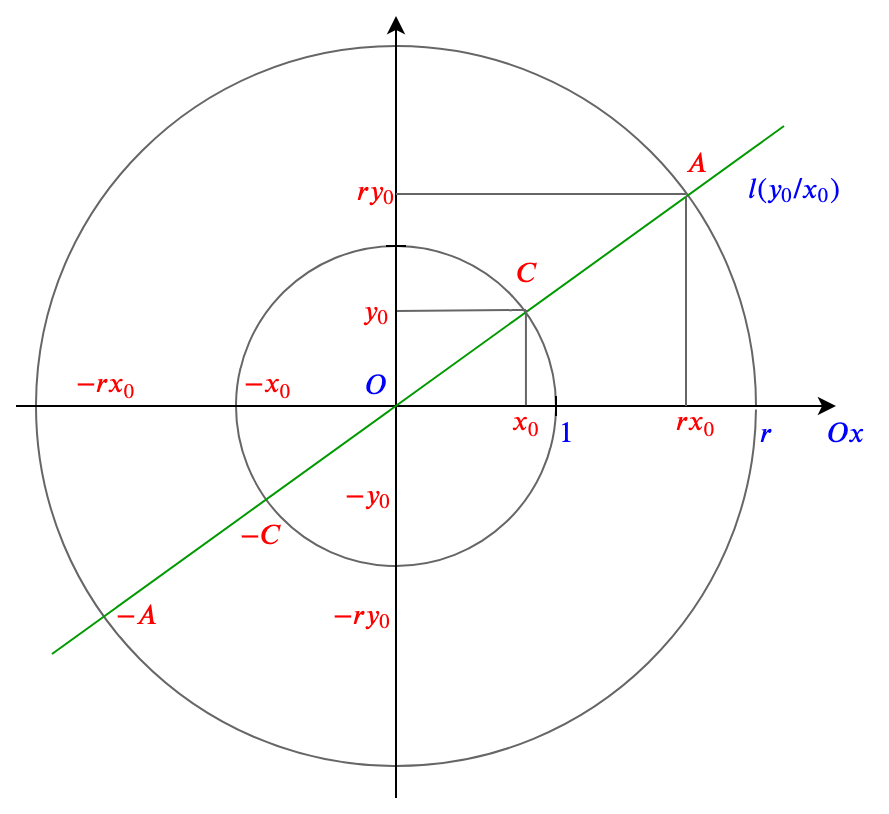
\includegraphics[scale=0.3]{line.png}
\end{center}
\item Этот вывод можно получить и более формально, просто глядя на уравнение прямой
$$
xy_0-yx_0=0.
$$
Ведь если мы домножим обе части уравнения на $r$, ничего не изменится!
$$
x(ry_0)-y(rx_0)=0.
$$
\item Что если прямая $l$ не проходит через центр координат $O$? В этом случае мы можем сдвинуть ее на некоторый вектор так, чтобы произвольно выбранная точка этой прямой перешла в точку $O$. Обозначим эту точку на прямой $l$ за $S=(\De x,\De y)$, а сдвиг, соответственно, осуществим на вектор $(-\De x,-\De y)$.
\begin{center}
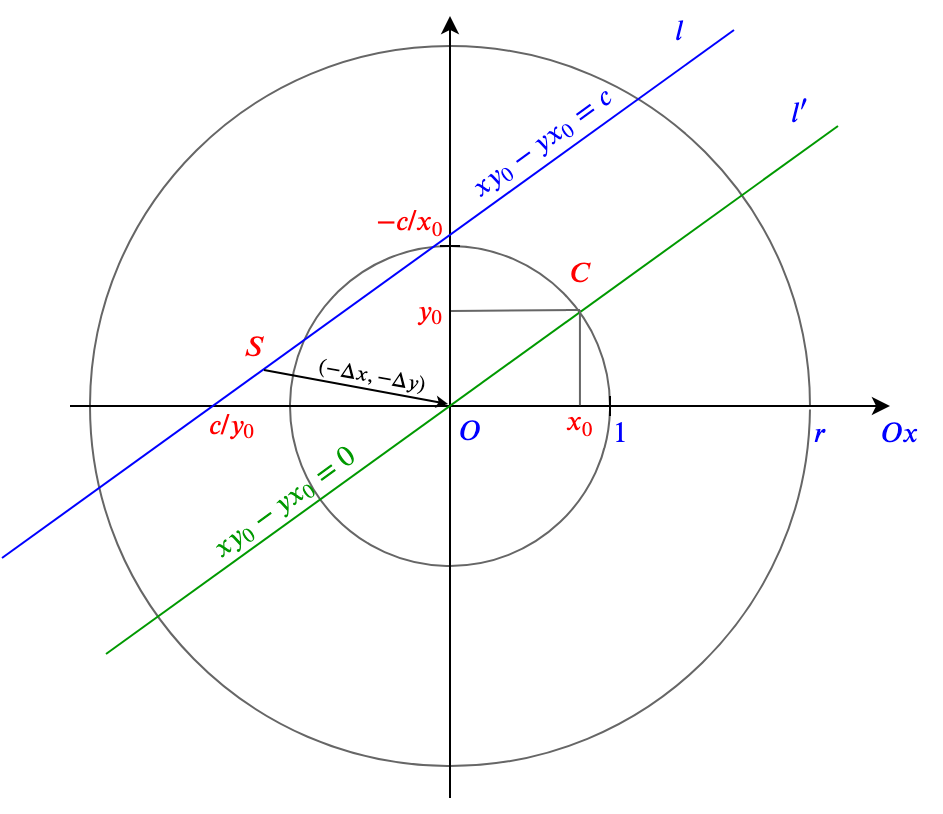
\includegraphics[scale=0.3]{lineshift.png}
\end{center}
\item Тогда смещенные координаты $(x-\De x,y-\De y)$ уже будут пробегать прямую $l'$, проходящую через центр $O$, а ее уравнение нам известно:
$$
(x-\De x)y_0 - (y-\De y)x_0=0,
$$
или
$$
xy_0-yx_0=c,\quad\mbox{где } c= y_0\De x - x_0\De y.
$$
При этом коэффициенты $(x_0,y_0)$ все так же отвечают за наклон прямой $l$ и полностью определяются тангенсом угла наклона прямой $l$ относительно положительного направления $Ox$, т.е. отношением $y_0/x_0$.
\item Может показаться, что уравнение сильно зависит от выбора точки $S$, поскольку слагаемое $c$ зависит от координат точки $S$. Покажем, что это не так. Пусть $S'=(\De x',\De y')$ --- какая-то другая точка прямой $l$. Но в этом случае она удовлетворяет найденному уравнению, т.е.
$$
\De x'y_0-\De y'x_0=c,
$$
но уравнение, найденное с помощью точки $S'$ будет иметь вид
$$
xy_0-yx_0= y_0\De x' - x_0\De y',
$$
откуда из предыдущего получаем, что вновь
$$
xy_0-yx_0=c.
$$
\item Таким образом, для нахождения $c$ мы можем выбрать любую понравившуюся нам точку прямой $l'$, например, отчку пересечения с одной из координатных осей.
\item В случае, когда $x_0\ne 0$, уравнение прямой можно переписать в виде
$$
y  = ax+b,\quad\mbox{где }a=\frac{y_0}{x_0},\; b=-\frac{c}{x_0}.
$$
В случае $x_0=0$ мы имеем вертикальную прямую $x=c$ (при угле $\ph=\pi/2$ мы получим $y_0=1$).
\end{enumerate}
\subsection*{Задачи}

\begin{enumerate}
\item В какие точки переходят точки $(0,3)$ и $(4,0)$ при повороте на $90$ градусов? На $-90$ градусов?
\item Каков угол поворота, если точка $(a,b)$ перешла в точку $(-a,-b)$? В точку $(-b,a)$? В точку $(b,-a)$?
\item Чему равен тангенс угла наклона прямой $3x-5y=7$?
\item Какой угол наклона у прямой $y=-x+3$?
\end{enumerate}


\section{Линейные уравнения в целых числах}

\subsection*{Конспект}

\begin{enumerate}
\item Поскольку мы пока владеем аппаратом только целых чисел (множество $\Z$), рассмотрим задачу о нахождении всех целых точек плоскости, через которые проходит заданная прямая. Под целыми точками плоскости мы будем понимать такие точки, координаты которых принадлежат $\Z$.
\item В общем виде \textbf{линейное уравнение в целых числах} выглядит следующим образом:
$$
ax-by=c,\quad\mbox{где коэффициенты } a,b,c\in\Z.
$$
Задача: найти все такие $x,y$, тоже целые, которые удовлетворяют данному уравнению.
\item Сначала рассмотрим случай т.н. \textbf{однородного уравнения}:
$$
ax-by=0,
$$
т.е. мы отбрасываем ту часть уравнения, которая не зависит от переменных $x,y$.
\item Как мы уже знаем, данное уравнение задает прямую, проходящую через начало координат, а ее наклон определяется отношением $a/b$.
\item Для начала проверим, нельзя ли данное отношение упростить. Если числа $a,b$ имеют какой-то общий делитель, то разумно было бы на него сократить. И чтобы не проверять это много раз, сократим их сразу на $\gcd(a,b)$. Множество решений от этого не изменится, а само уравнение по-прежнему останется однородным и целочисленным:
$$
\tilde ax-\tilde by=0,\quad\mbox{где } \tilde a=\frac{a}{\gcd(a,b)},\;\tilde b=\frac{b}{\gcd(a,b)}.
$$
\item Таким образом, мы приходим к уравнению со взаимно простыми коэффициентами $\tilde a$ и $\tilde b$.
\item Перепишем уравнение иначе: $\tilde ax=\tilde by$. Заметим, что все числа здесь --- целые. Причем $\tilde by$ делится на $\tilde a$. Но так как $\tilde a$ и $\tilde b$ взаимно просты, то $y$ делится на $\tilde a$. Это есть следствие того факта, который мы доказывали ранее в разделе \ref{PrimeNumbers}: если простое число $p$ делит произведение $ab$, то оно делит $a$ или $b$ (или их обоих). Поэтому если простое $p$ делит $\tilde a$, то оно делит $\tilde by$, но оно не может делить $\tilde b$, т.к. $\gcd(p,\tilde b)=1$, значит, оно делит $y$. Это значит, что все простые, составляющие число $\tilde a$, являются делителями $y$. В то же время, эти простые не входят в $\tilde b$, поскольку $\gcd(\tilde a,\tilde b)=1$. Поэтому, если $p^\al$ входит в разложение $\tilde a$, то $p^\al$ также делит $y$. Следовательно, $y$ делится на $\tilde a$, т.е. 
$$
y=k\tilde a
$$
при некотором целом $k$.
\item Симметрично рассуждая, получаем, что $x$ делится на $\tilde b$, т.е.
$$
x=t\tilde b
$$
при некотором целом $t$.
\item Подставим эти выражения в наше однородное уравнение:
$$
\tilde a(t\tilde b)=\tilde b(k\tilde a),
$$
откуда
$$
t=k,
$$
и больше никаких ограничений на выбор коэффициента $k$ мы не имеем.
\item Таким образом, решениями уравнения $\tilde ax-\tilde by=0$ являются
$$
\begin{cases}
x  =k\tilde b=kb/\gcd(a,b), \\
y  =k\tilde a=ka/\gcd(a,b),
\end{cases}
$$
где $k\in\Z$. Эти же $x$ и $y$ являются решениями исходного однородного уравнения $ax-by=0$.
\item Вернемся к неоднородному уравнению $ax-by=c$.
\item Для начала заметим, что если данное уравнение имеет решение в целых числах, то $ax-by$ делится на $\gcd(a,b)$, а значит, $c$ делится на $\gcd(a,b)$. Поэтому, если $c$ не делится на $\gcd(a,b)$, то решений точно нет, т.е. в таком случае прямая $ax-by=c$ проходит мимо всех целых точек плоскости!
\item Покажем, что в случае делимости $c$ на $\gcd(a,b)$ решения обязательно есть, и опишем все такие решения.
\item Пусть $c=d\gcd(a,b)$.
\item В разделе \ref{PrimeNumbers} мы установили, что $\gcd(a,b)$ является линейной комбинацией чисел $a$ и $b$, т.е.
$$
\gcd(a,b) = an-bm
$$
при некоторых целых $n$ и $m$ (понятно, что знак перед $m$ можно выбирать любой, поэтому выберем так, как нам удобнее).
\item Отсюда следует, что пара чисел $(dn,dm)$ удовлетворяет уравнению $ax-by=c$, поскольку
$adn-bdm=d\gcd(a,b)=c$.
\item Итак, представив $\gcd(a,b)$ в виде линейной комбинации $a$ и $b$, мы можем найти одно решение исходного уравнения.
\item Далее применим тот же прием, что и при изучении уравнений прямых --- сдвинем прямую $ax-by=c$ так, чтобы точка $(dn,dm)$ оказалась в начале координат. Для этого введем новые переменные
$$
\hat x = x-dn,\quad \hat y = y-dm.
$$
\item Тогда получаем, что $a\hat x-b\hat y = 0$. А такое уравнение мы уже решили выше, и его решением будет пара чисел $\hat x = kb/\gcd(a,b)$ и $\hat y = ka/\gcd(a,b)$, где $k$ --- любое целое число.
\item Собирая все вместе, находим общее решение исходного уравнения:
$$
\begin{cases}
x  =kb/\gcd(a,b) + dn, \\
y  =ka/\gcd(a,b) + dm,
\end{cases}
$$
\item Таким образом, решением линейного уравнения $ax-by=c$ в целых числах является сумма общего решения однородного уравнения $ax-by=0$ и какого-нибудь частного решения исходного уравнения.
\item Основной трудностью при поиске частного решения является нахождение коэффициентов $n$ и $m$ представления $\gcd(a,b)$.
\item Это представление можно найти с помощью алгоритам Евклида. Рассмотрим для примера уравнение
$$
18x-11y=2
$$
\item Следуя алгоритму Евклида, получаем выкладки:
\begin{align*}
18 = & 11\cdot 1+7,\\
   & 11 = 7\cdot 1 + 4, \\
   & 7 = 4\cdot 1 + 3, \\
   & 4 = 3\cdot 1 + 1
\end{align*}
Последняя 1 --- это и есть $\gcd(18,11)$. Раскрутим алгоритм в обратную сторону:
\begin{align*}
1 & = 4-3 = 4 - (7-4) = 4\cdot 2-7 = (11-7)\cdot 2-7 =\\
  & = 11\cdot 2-7\cdot 3 = 11\cdot 2 - (18-11)\cdot 3 =\\
  & = 11\cdot 5 - 18\cdot 3.
\end{align*}
Таким образом, наши искомые числа $n=-3$, $m=-5$. Напомним, что мы ищем представление $\gcd(18,11)$ в виде $18n-11m$, исходя из чего нужно правильно выбирать знаки перед коэффициентами.

Кроме того, $d=2$, т.к. $c=2$ и $\gcd(a,b)=1$. Откуда общее решение уравнения $18x-11y=2$ получаем в виде:
$$
\begin{cases}
x  =11k - 6, \\
y  =18k - 10,
\end{cases}
$$
где $k$ --- любое целое число. Проверим:
$$
18(11k - 6) - 11(18k - 10) = 198k-198k - 108 + 110 =2.
$$
\item Наконец, приведем еще один замечательный способ найти разложение НОД. Этот метод основан на представлении дробей в виде т.н. \textbf{цепных дробей}. Пусть дано уравнение
$$
112x-34y=16.
$$
\item Ищем приближение дроби $112/34$ следующим способом:
$$
\frac{112}{34} = 3 + \frac{5}{17} = 3 + \frac{1}{3+\frac{2}{5}} = 
3 + \frac{1}{3 + \frac{1}{2+1/2}}
$$
По сути дела, это --- другая запись выкладок алгоритма Евклида, поскольку мы каждый раз последовательно выделяем неполное частное предыдущих остатков.

Как только мы дошли до хвоста вида $1/k$, мы останавливаемся, отбрасываем этот хвост и сворачиваем дробь обратно, получая приближение исходной дроби:
$$
\frac{112}{34} \approx 3 + \frac{5}{17} = 3 + \frac{1}{3+\frac{2}{5}} = 
3 + \frac{1}{3 + \frac{1}{2}} = \frac{23}{7}
$$
Далее, перемножая накрест эти дроби, получаем представление для НОД:
$$
\gcd(112,34) = 112\cdot 7 - 34\cdot 23.
$$
Искомые коэффициенты: $n=7$, $m=23$. Общее решение уравнения, таким образом, получаем в виде
$$
\begin{cases}
x  = 34k +  8\cdot 7, \\
y  = 112k + 8\cdot 23 ,
\end{cases}
$$
где $k$ --- любое целое число, а $8=16/\gcd(112,34)$. Проверяем:
$$
112(34k +  8\cdot 7)-34(112k + 8\cdot 23) = 8(112\cdot 7- 34\cdot 23) = 16.
$$
\item Выше мы всюду рассматривали уравнения, в которых $x$ идет с положительным коэффициентом, а $y$ --- с отрицательным. Иначе говоря, прямая, заданная таким уравнением, имеет наклон <<вправо>>. Но уравнение может быть, например, таким
$$
5x+9y=1.
$$
Если мы хотим решать его по тем же формулам, то лучше перейти к новым переменным $\hat x=x$, $\hat y=-y$, и тогда мы получим уравнение
$$
5\hat x-9\hat y=1.
$$
Найдя его решения, мы просто меняем знак у $\hat y$, и получаем исходное уравнение.
\end{enumerate}

\subsection*{Задачи}

\begin{enumerate}
\item Найти представление $\gcd(5,9)$ с помощью алгоритма Евклида и методом цепных дробей.
\item Найти представление $\gcd(18,15)$ с помощью алгоритма Евклида и методом цепных дробей.
\item Найти представление $\gcd(225,81)$ с помощью алгоритма Евклида и методом цепных дробей.
\item Решить уравнение $5x-9y=2$ в целых числах.
\item Найти все решения уравнения $225x+81y=18$ в целях числах.
\item Найти все решения уравнения $10x-18y=3$ в целях числах или доказать, что их нет.
\end{enumerate}



\chapter{Числовые поля}

\vrezka{
В этой главе мы ачинаем выход за пределы целых чисел, и прежде всег займемся построением чисел рациональных. Кроме того, здесь будет введено определение поля и приведены примеры конечных полей.
}


\section{Рациональные числа}

\subsection*{Конспект}
\begin{enumerate}
\item Предыдущую главу мы закончили действиями с дробями, хотя нигде до сих пор о них не говорили. Разве что, упоминали отношение $y_0/x_0$ как некоторый параметр, определяющий угол наклона прямой на координатной плоскости.
\item Итак, рассмотрим прямую $l$, заданную уравнением $ax-by=0$, где $a,b$ --- целые числа.
\item Для начала пусть $a=1$ и $b>1$. Легко видеть, что такая прямая проходит через точки $(0,0)$ и $(b,1)$ (см. рис.).
\begin{center}
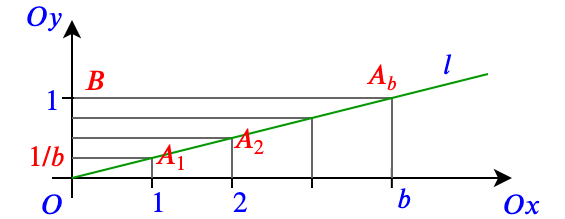
\includegraphics[scale=0.5]{section.png}
\end{center}
\item На прямой $l$ мы можем поставить точки $A_1, A_2, \dots, A_b$ в местах пересечения этой прямой с вертикальными прямыми, имеющими уравнения $x=1, x=2, \dots, x=b$, соответственно.
\item Теперь рассмотрим треугольник $OBA_b$, где точка $B=(0,1)$. В этом треугольнике мы можем провести линии, параллельные его горизонтальной стороне $BA_b$, которые отсекут на вертикальной стороне $OB$ нашего треугольника отрезки.
\item Эти отрезки будут иметь одинаковую длину по теореме Фалеса, т.к. точки на прямой $l$ также расставлены с одинаковым шагом, что следует уже из выбора вертиклаьных секущих (они идут с шагом 1).
\item Итак, на вертикальной оси мы получили $b$ одинаковых отрезков, сумма длин которых равна 1.
\item Какова же длина каждого из таких отрезков? Ответ: она равна одной $b$-ой части единицы. И эта часть записывается как дробь $1/b$. Собственно, отношение $1/b$, как мы видели ранее, является определяющим для прямой $l$.
\item Мы можем брать сумму нескольких таких частей, например, $k$ частей размера $1/b$ дают в сумме отрезок длины в $k$ раз больше, чем отрезок $1/b$. Такая часть записывается в виде дроби $k/b$.
\item Величину $k/b$ можно получить иным способом. Возьмем теперь прямую $l'$, заданную уравнением $kx+by=0$ (см. рис.).
\begin{center}
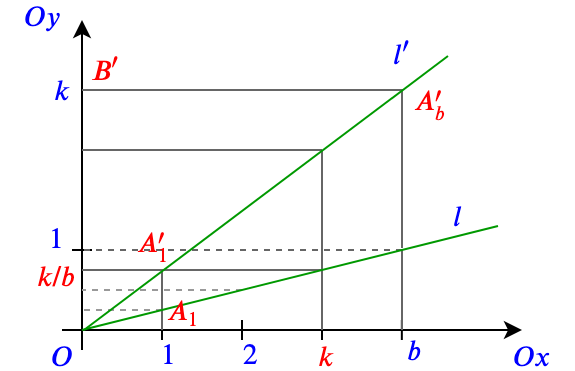
\includegraphics[scale=0.5]{sectionkb.png}
\end{center}
\item Эта прямая проходит через начало координат и точку $(b,k)$.
\item Проделаем аналогичные предыдущему построения: проведем вертикальные линии с шагом 1, а затем горизонтальные линии от точек пересечения вертикальных с прямой $l'$, и посмотрим, какие отрезки у нас получатся на оси $Oy$.
\item Нетрудно видеть, что линия, соответствующая $x=k$, для прямой $l$ отсекает на оси $Oy$ метку, которую мы обозначили как $k/b$. Но ровно ту же самую метку покажет построение с помощью вертикальной линии $x=1$ и прямой $l'$. Почему? А очень просто: достаточно сравнить уравнения этих прямых
$$
l:\;x-by=0,\quad l':\;kx-by=0.
$$
Если в первом вместо $x$ подставить $k$, а во втором вместо $x$ подставить 1, то получим одно и то же значение $y$. Отсюда и совпадение меток.
\item Таким образом, прямая $l'$ дает на оси $Oy$ шаг в $k$ раз больше, чем прямая $l$, если мы строим сечения при одном и том же $x$ (не обязательно $x=1$).
\item Получается, что прямая, заданная уравнением $kx-by=0$, задает умножение на число $k$ всех чисел, получаемых прямой, заданной уравнением $x-by=0$.
\item Рассматривая эти прямые как некие \textit{новые объекты}, мы можем ввести понятие умножения прямой на целое число. Если у нас есть прямая $\{ax-by=0\}$, то результатом ее умножения на число $k$ является прямая $\{kax-by=0\}$. Запишем это так:
$$
k\{ax-by=0\} = \{(ka)x-by=0\}.
$$
\item Заметим, что сложение (и вычитание) таких прямых определить еще проще: 
$$
\{a_1x-by=0\}\pm\{a_2x-by=0\} = \{(a_1\pm a_2)x-by=0\}.
$$
\textbf{Важно:} при сложении прямых коэффициент перед $y$ должен быть одинаковым у обеих прямых!
Только в этом случае мы получаем согласование операций сложения и умножения, а именно:
$$
\underbrace{\{ax-by=0\}+\dots+\{ax-by=0\}}_{k\mbox{ раз}} = \{kax-by=0\} = k\{ax-by=0\},
$$
\item Сложение прямых можно интерпретировать графически как сложение площадей прямоугольников с основанием $b$ и высотой $a_1$ и $a_2$. В результате получается прямоугольник с тем же основанием $b$ и высотой $a_1+a_2$. При этом прямые всегда проходят через точку $(0,0)$ и правый верхний угол прямоугольников.
\begin{center}
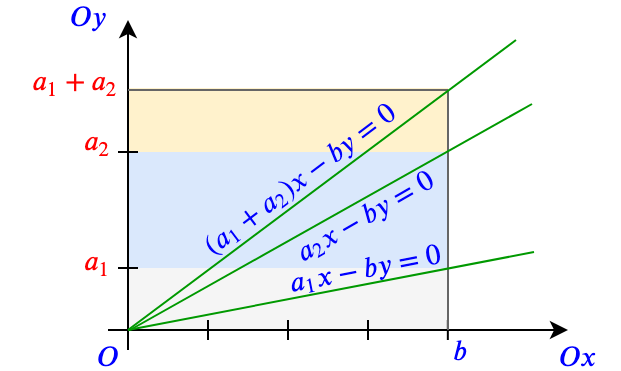
\includegraphics[scale=0.5]{linesum.png}
\end{center}
С помощью этой же картинки можно представить себе и умножение прямой на целое число $k$. Для этого нужно растиражировать соответствующий этой прямой прямоугольник вверх $k$ раз.

\item На самом же деле операции сложения, вычитания и умножения на целое число, производимые с коэффициентом перед $x$, в точности повторяют таковые операции над целыми числами (поскольку это и есть целые числа!) и, соответственно, подчиняются всем аксиомам кольца целых чисел. [А вот и более умный термин для тех, кто собирается идти в математику глубоко: \textit{прямые с общим основанием $b$ образуют векторное пространство над кольцом} $\Z$.]
\item Поэтому все прямые вида $ax-by=0$ при фиксированном $b\ne 0$ с определенныими выше операциями сложения и умножения \textit{образуют кольцо} (изоморфное кольцу целых чисел). 
\item Если вместо сложной записи $ax-by=0$, описывающей прямую, записать просто отношение $a/b$, то мы увидим, что операции с прямыми образуют в точности операции с дробями:
$$
k\frac{a}{b}  = \frac{ka}{b}\quad\mbox{и}\quad\frac{a_1}{b}+\frac{a_2}{b} = \frac{a_1+a_2}{b}.
$$
\item Заметим теперь, что уравнение $x-by=0$ прямой $l$ можно переписать иначе: $kx-(bk)y=0$. Чем оно отличается от уравнения $kx-by=0$ прямой $l'$? Очевидно, тем, что перед $y$ появился коэффициент $k$. А тепрь вспомним, что прямая $l$ задает отношение в $k$ раз меньше, чем прямая $l'$! И это значит, что если мы хотим разделить прямую $l'$ на $k$, то мы должны умножить на $k$ ее коэффициент перед $y$.
\item Итак, если мы хотим умножить прямую на число, то мы умножаем на это число коэффициент перед $x$ (прямая становится более крутой), а если мы хотим разделить прямую на число, то мы умножаем на это число коэффициент перед $y$ (прямая становится более пологой).
\item Делаем следующий шаг: умножение двух прямых. На самом деле, любую прямую $ax-by=0$ мы можем переписать как серию ранее определенных операций:
$$
\{ax-by=0\} = a\{x-y=0\}/b,
$$
при этом прямая $x-y=0$ имеет наклон 45 градусов и соответствует отношению 1/1, т.е. по-просту 1, и в операциях умножения может опускаться. Таким образом, умножение прямых выглядит следующим образом
\begin{gather*}
\{a_1x-b_1y=0\}\cdot\{a_2x-b_2y=0\} = \\
= a_1\{x-y=0\}/b_1\cdot a_2\{x-y=0\}/b_2 = \{a_1a_2x-b_1b_2y=0\},
\end{gather*}
а это в точности умножение дробей: $(a_1/b_1)(a_2/b_2) = (a_1a_2)/(b_1b_2)$.
\item Отсюда нетрудно получить и процедуру деления прямых друг на друга:
$$
\{a_1x-b_1y=0\}/\{a_2x-b_2y=0\} = \{(a_1b_2)x-(a_2b_1)y=0\},
$$
что соответствует операции с дробями:
$$
\frac{a_1}{b_1}/\frac{a_2}{b_2} = \frac{a_1b_2}{a_2b_1}.
$$
\item Наконец, чтобы научиться складывать произвольные прямые, мы должны уметь сводить сложение произвольных прямых к сложению прямых с одинаковым коэффициентом перед $y$, т.к. сложение мы определили выше только для данного случая.
\item Но и это не проблема:
\begin{gather*}
(a_1x-b_1y=0)+(a_2x-b_2y=0) = (a_1b_2x-b_1b_2y=0) + (a_2b_1x-b_1b_2y=0) = \\
= ((a_1b_2+a_2b_1)x-(b_1b_2)y=0),
\end{gather*}
что соответствует операциям с дробями
$$
\frac{a_1}{b_2}+\frac{a_2}{b_2} = \frac{a_1b_2+a_2b_1}{b_1b_2}.
$$
\item Следующая картинка показывает <<арифметику прямых>> с произвольными параметрами.
\begin{center}
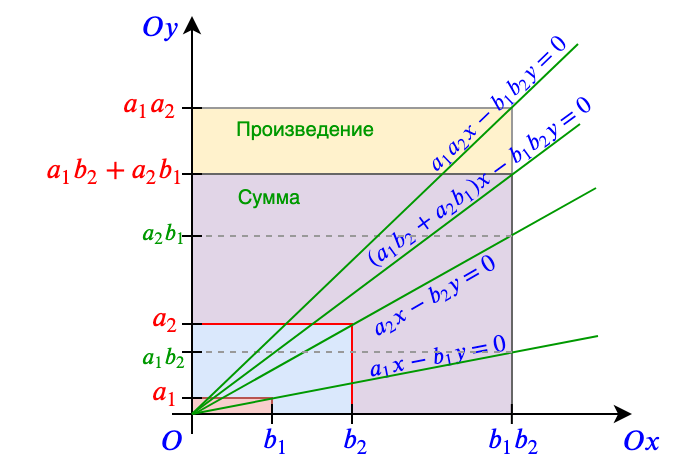
\includegraphics[scale=0.5]{linear.png}
\end{center}
Здесь маленькие прямоугольники соответствуют исходным прямым с уравнениями $a_1x-b_1y=0$ и $a_2x-b_2y=0$, пунктиром отмечены приведенные к общему основанию $b_1b_2$ прямоугольники, большой темный прямоугольник соответствует их сумме (буквально однин приставлен сверху к другому), большой светлый прямоугольник --- произведению (помножены основания и помножены высоты). Рисунок не учитывает масштаб!

\item В целом картина представления рациональных чисел с помощью прямых с целочисленными коэффициентами выглядит следующим образом:
\begin{center}
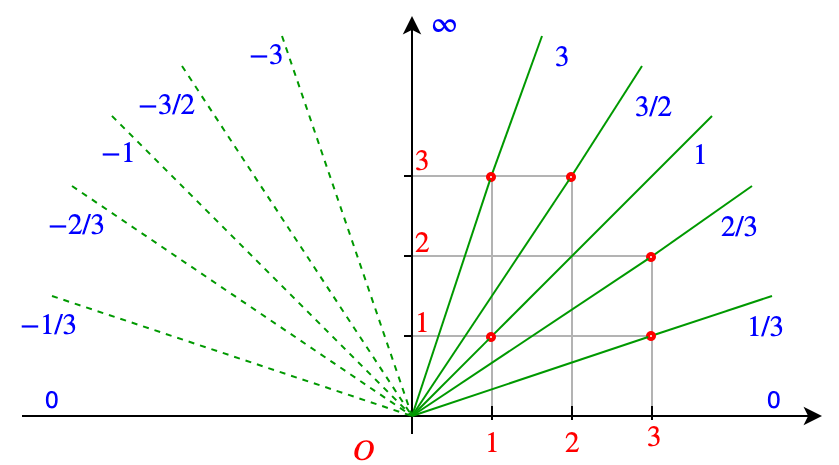
\includegraphics[scale=0.4]{ratio.png}
\end{center}

\item Итак, имея только множество целых чисел $\Z$, мы построили на плоскости всевозможные прямые, заданные линейными уравнениями с целыми коэффициентами, научились их складывать, вычитать, умножать и делить. Тем самым, мы построили новую алгебраическую структуру, которая называется \textbf{полем}. Поле --- это кольцо, в котором можно делить на любое число, кроме нуля.
\item Записывая эти прямые не уравнениями, а отношением коэффициентов (вместо $ax-by=0$ пишем $a/b$), мы получаем \textbf{поле рациональных чисел}, которое принято обозначать $\Q$.
\item На самом деле, в нашем построении есть еще и такая прямая, которая соответствует бесконечности. Это прямая, заданная уравнением $x=0$. А нулевая прямая определяется уравнением $y=0$. В полном соответствии с установленными правилами, мы можем заметить, что если $a\ne 0 \ne b$, то
\begin{gather*}
\{ax-by=0\}\{y=0\}=\{y=0\},\;\{ax-by=0\}\{x=0\}=\{x=0\},\\ 
\{ax-by=0\}/\{y=0\}=\{x=0\},\;\{ax-by=0\}/\{x=0\}=\{y=0\},
\end{gather*}
или, иначе:
$$
\frac{a}{b}\cdot 0 = 0,\quad\frac{a}{b}\cdot\infty = \infty,\quad
\frac{a}{b}/ 0 = \infty,\quad\frac{a}{b}/\infty = 0
$$
при $a\ne 0\ne b$,
т.е. деление на ноль дает бесконечность, а деление на бесконечность дает ноль.
\item Но тут кроется проблема: $\{x=0\}\cdot\{y=0\}=\{0x-0y=0\}$ --- такое уравнение на задает прямую, его решением является вся плоскость! Проще говоря, при умножении $0\cdot\infty$ может получиться любое число!
\item Поэтому при определении поля бесконечный элемент не постулируется и, соответственно, деление на ноль не разрешено.
\item Приведем полный формальный список аксиом поля. Множество $F$ с операциями $+$ и $\cdot$ называется \textbf{полем}, если:
\begin{enumerate}[{\bf Field}1]
\item $a,b\in F\Rightarrow a+b\in F, a\cdot b\in F$ (замкнутость операций);
\item $a,b,c\in F\Rightarrow (a+b)+c=a+(b+c), (a\cdot b)\cdot c = a\cdot (b\cdot c)$ (ассоциативность операций);
\item для всех $a,b\in F$ имеем $a+b=b+a$ и $a\cdot b=b\cdot a$ (коммутативность операций);
\item существует элемент $0\in F$ такой, что $a+0=0+a=a$ для всех $a\in F$ (аксиома нуля);
\item для всякого элемента $a\in F$ существует противоположный $-a$ такой, что $a+(-a)=0$ (аксиома противоположного элемента);
\item существует элемент $1\in F$ такой, что $a\cdot 1=1\cdot a=a$ для всех $a\in F$ (аксиома единицы),
\item для всякого элемента $a\in F$, если $a\ne 0$, то существует обратный $a^{-1}$ такой, что $a\cdot a^{-1}=1$ (аксиома обратного элемента).
\item для всех $a,b,c\in F$ имеем $(a+b)\cdot c=(a\cdot c)+(b\cdot c)$, $c\cdot(a+b)=(c\cdot a)+(c\cdot b)$ (правая и левая дистрибутивность);
\end{enumerate}
\item Иначе говоря, поле --- это \textit{коммутативное кольцо с единицей, в котором каждый ненулевой элемент обратим}. На следующей схеме представлено формирование таких понятий как поле и кольцо из более простых свойств (или аксиом):
\begin{center}
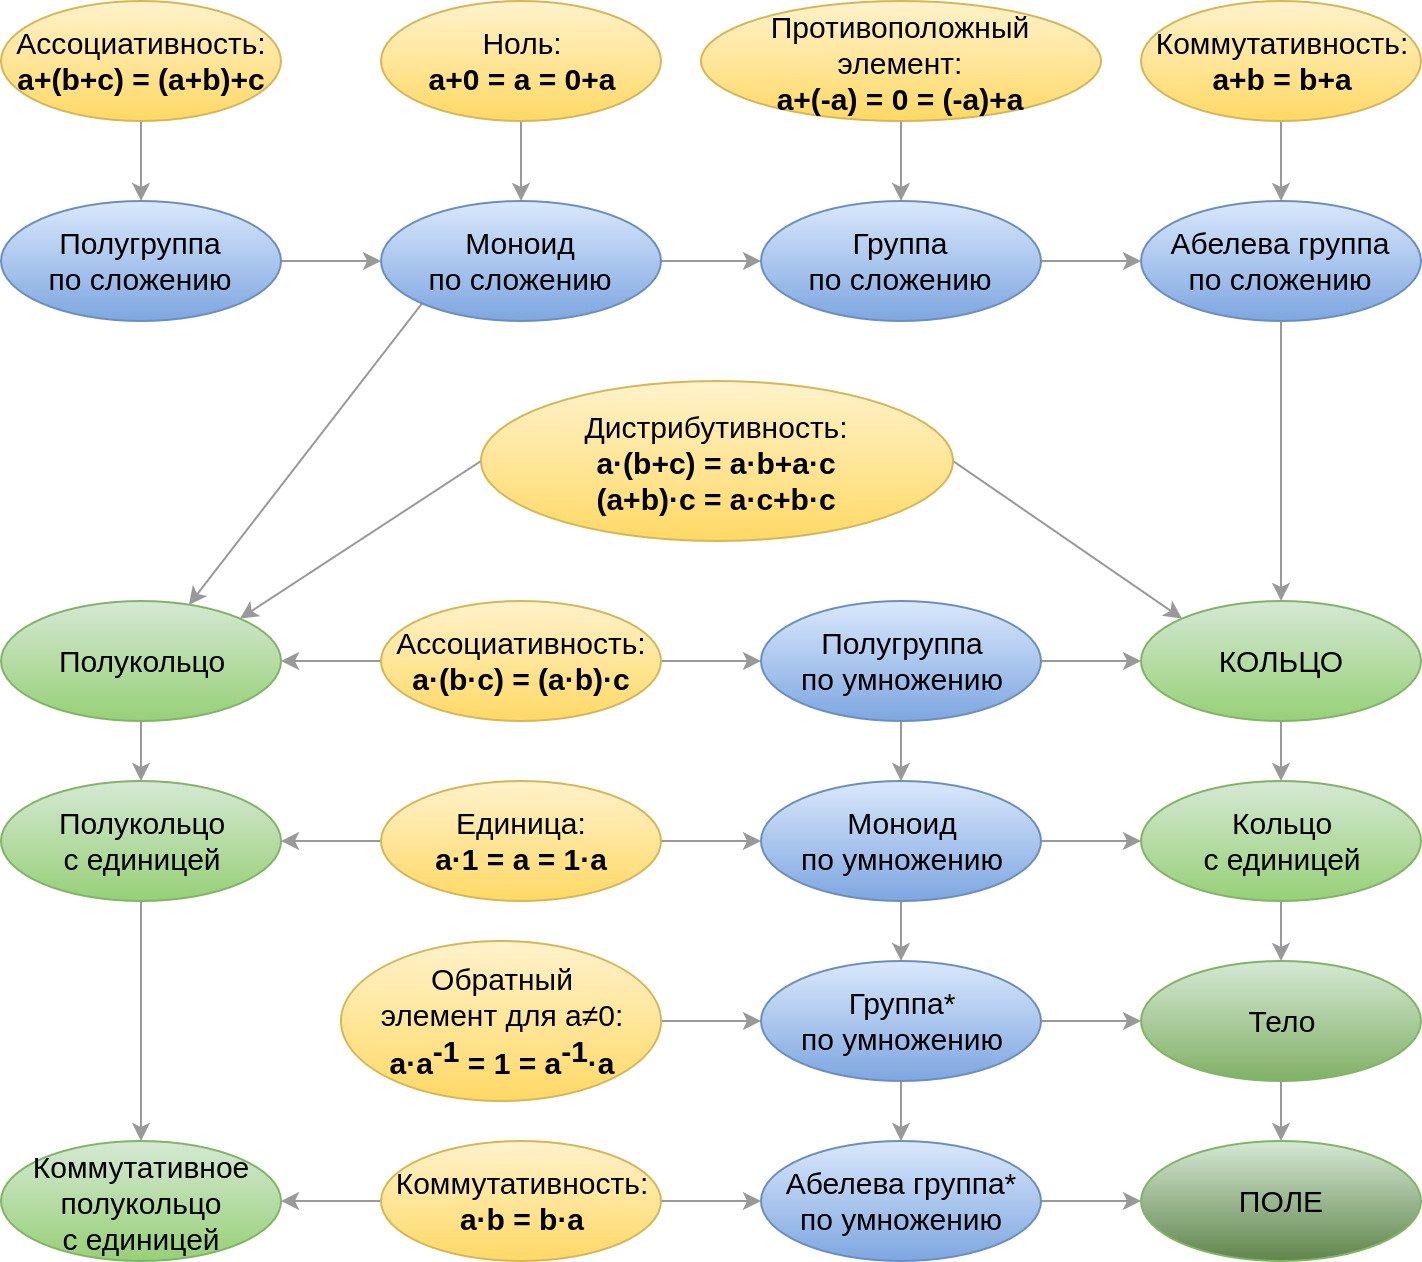
\includegraphics[scale=0.25]{Ring.png}
\end{center}
\end{enumerate}


\subsection*{Задачи}





\section{Соизмеримость. Иррациональности}

\subsection*{Конспект}

\begin{enumerate}
\item Рациональные числа мы построили с помощью прямых, заданных уравнением $ax-by=0$, где $a$ и $b$ --- произвольные целые числа, одновременно не равные нулю. Оказалось, что такая прямая отсекает отрезки длины $a/b$ на вертикальной оси, когда $x$ меняется с шагом 1, т.е. пробегает все целые числа. В частности, при $x=1$ мы получаем уравнение $by=a$, решением которого является единственное число $y=a/b$.
\item Говоря алгебраическим языком, рациональные числа --- это корни линейных уравнений, т.е. уравнений вида $a-by=0$, с целыми коэффициентами $a,b$.
\item Таким образом, выход в поле рациональных чисел происходит при попытке разрешить линейное уравнение, заданное над кольцом целых чисел.
\item Что если мы рассмотрим линейное уравнение, но над полем рациональных чичел? Будет ли оно разрешимо?
\item Пусть $rx-q=0$ и $r,q\in\Q$. Тогда представим эти рациональные числа в виде дробей $r=a/b$, $q=c/d$, откуда
$$
0=rx-q = \frac{a}{b}x-\frac{c}{d} = \frac{adx-cb}{bd},
$$
откуда ясно, что данное уравнение эквивалентно линенойму уравнению $(ad)x-(cb)=0$ с целыми коэффициентами, а значит, разрешимо в поле рациональных чисел.
\item Таким образом, поле $\Q$ замкнуто относительно линейных уравнений. Посмотрим, как оно справится с уравнениями более высокой степени! Рассмотрим уравнение $x^2-2=0$. Это уравнение с целыми коэффициентами (1 и 2). Разрешимо ли оно в $\Z$ или хотя бы в $\Q$?
\item Ответ: нет! Предположим, что $x=n/m$ разрешает такое уравнение, т.е. $(n/m)^2=2$. Предположим сразу же, что $n\perp m$, т.е. дробь $n/m$ несократимая. Далее имеем
$$
n^2=2m^2.
$$
Отсюда видно, что $n^2$ делится на 2, а значит, $2$ входит в разложение числа $n^2$ по степеням простых. Проблема в том, что если бы 2 не входила в разложение числа $n$, то ее не было бы и в разложении числа $n^2$, т.к. $n^2$ есть поризведение степеней тех же самых простых, что и $n$, только в удвоенной степени. А значит, $n$ делится на 2, откуда следует, что $n^2$ делится на 4. Но тогда $m^2$ делится на 2 и, аналогично рассуждая, получаем, что и $m$ делится на 2. А это уже противоречит тому, что дробь $n/m$ несократимая --- ее как минимум можно сократить на 2.

Следовательно, корень уравнения $x^2-2=0$ не может быть рационалным числом.
\item Тем не менее, положительный корень такого уравнения можно оценивать сверху и снизу сколь угодно точно. Например, корень извлекается из числа 2.25 и равен 1.5, при этом $x^2=2<2.25$, так что $x<1.5$. В то же время, $2>1.96=1.4^2$, так что $x>1.4$. Можно еще усилить оценку: $1.41<x<1.42$. И так далее. Это позволяет нам думать, что на самом деле число такое есть, просто оно сидит где-то между рациональными числами. Обоснование его существования мы отложим на потом, а пока просто обозначим его $\sqrt 2$.
\item Есть ее один способ удостовериться в том, что $\sqrt 2$ не является рациональным числом. И тут снова нам на выручку приходят цепные дроби. Теперь-то мы вправе ими оперировать!
\item Воспроизведем алгоритм Евклида для дроби $\al = r_0/r_1$, считая, что $r_0>r_1$ (если это не так, то приведем дробь к виду $1/(r_1/r_0)$ и будем работать дальше только со знаменателем). Как и раньше, будем выделять остаток $r_{k+1}$ от деления $r{k-1}$ на $r_k$ и сохранять неполное частное $m_k$. Только запишем весь алгоритм не в несколько строк, а в виде многоэтажной дроби. Поехали!
\begin{multline*}
\frac{r_0}{r_1} = \frac{k_1r_1+r_2}{r_1} = \boxed{k_1}+\frac{1}{\frac{r_1}{r_2}} =
\boxed{k_1} + \frac{1}{\frac{k_2r_2+r_3}{r_2}} =  \\
= \boxed{k_1} + \frac{1}{\boxed{k_2} + \frac{1}{r_3/r_2}} = 
\boxed{k_1} + \frac{1}{\boxed{k_2} + \frac{1}{\boxed{k_3} + \ddots \frac{1}{\boxed{k_n}+r_{n+1}/r_n}}},
\end{multline*}
где $r_0>r_1>r_2>\dots>r_n>r_{n-1}$.

\item Поскольку остатки всегда являются натуральными числами, рано или поздно этот алгоритм прервется. Пусть это случится на шаге с номером $n$, так что мы полагаем $r_{n+1}=0$, и цепная дробь закончится на числе $k_n$.
\item В таком случае цепную дорбь принято записывать последовательностью выделенных на каждом шаге целых частей:
$$
\frac{r_0}{r_1} = [k_1,k_2,\dots,k_n].
$$
\item Отсюда следует, что всякая рациональная дробь представима в виде конечной цепной дроби. Обратное, очевидно, также верно, ибо каждую конечную цепную дробь можно свернуть по правилам арифметики в обычную рациональную дробь.
\item Заметим также, что любое целое число представлятся в виде тривиальной цепной дроби, в которой есть только $k_1$.
\item Алгоритм Евклида можно применять к любым числам, лишь бы можно было выделять остаток от деления. Например, его можно применить к паре чисел $\pi/2$ и $\pi/3$ и получить конечную цепную дробь. А все потому, что отношение этих чисел является рациональным числом $3/2$. Поэтому, если отношение двух чисел $a/b$ рационально, их принято называть \textbf{соизмеримыми}.
\item\label{soizm} Соизмеримые числа хорошо иллюстрируются следующей картинкой:
\begin{center}
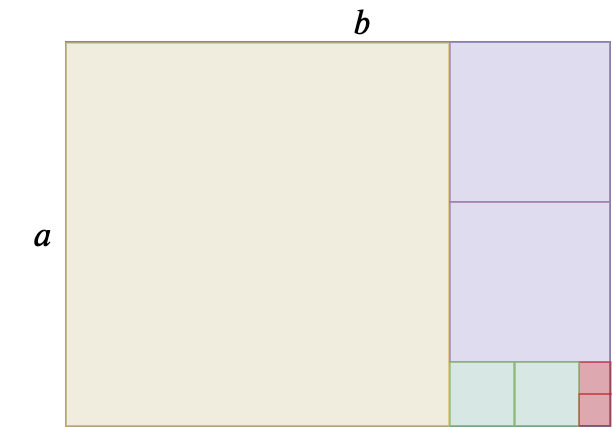
\includegraphics[scale=0.3]{soizmer.png}
\end{center}
Видим, что прямоугольник $a\times b$ мы делим на квадраты, каждый раз выбирая максимальный квадрат, который вписывается в оставшуюся область. Если $a$ и $b$ соизмеримы, то порцесс разрзания прямоугольника на квадраты закончится за конечное число шагов, причем количество одинаковых квадратов, посчитанное в порядке их убывания, есть как раз те самые числа $k_1,k_2,\dots,k_n$, появляющиеся в записи цепной дроби. Поскольку вырезание макисмального квадрата --- это не что иное как процесс выделения целой части из остатка, т.е. алгоритм Евклида.
\item То, что сами числа $a$ и $b$ при этом могт не быть целыми или рациональными --- не важно. Важно, что их отношение рационально. Также легко видеть, что всякое рациональное число соизмеримо с 1 и, наоборот, всякое число, соизмеримое с 1, рационально.
\item Посмотрим теперь, что происходит при попытке записать цепную дробь для $\sqrt 2$.
\item Мы уже знаем, что $1<\sqrt 2<2$, кроме того, $(\sqrt 2+1)=1/(\sqrt 2-1)$ так что
\begin{multline*}
\sqrt 2 = \boxed{1} + (\sqrt 2-1) = \boxed{1} + \frac{1}{1/(\sqrt 2-1)} = 
\boxed{1} + \frac{1}{\sqrt 2+1} = \\ 
= \boxed{1} + \frac{1}{\boxed{2} + (\sqrt 2-1)} = 
\boxed{1} + \frac{1}{\boxed{2} + \frac{1}{\sqrt 2+1}} = 
\boxed{1} + \frac{1}{\boxed{2} + \frac{1}{\boxed{2} + \frac{1}{\boxed{2} + \dots}}}
\end{multline*}
\item Как видим, остатком после выделения целой части всегда является одно и то же число $\sqrt 2-1$, и процесс алгоритма Евклида никогда не остановится. При этом цепная дробь характеризуется последовательностью одинаковых целых частей, равных 2. То есть представление для корня из 2 в виде цепной дроби будет бесконечным:
$$
\sqrt 2 = [1,2,2,2,2,2,\dots],
$$
и, следовательно, $\sqrt 2$ не является рациональным числом.
\item Числа, не яляющиеся рациональными, называются \textbf{иррациональными}.
\item Наличие иррационального числа $\sqrt 2$ позволяет нам рассмотреть числа вида $r+q\sqrt 2$, где $r,q\in\Q$.
\item Множество таких чисел, полученных присоединением к полю $\Q$ положительного корня уравнения $x^2=2$, принято обозначать $\Q[\sqrt 2]$ и называть расширением поля $\Q$.
\item Очевидно, что множество $\Q[\sqrt 2]$ замкнуто относительно сложения и вычитания, т.к.
$$
(r_1+q_1\sqrt 2)+(r_2+q_2\sqrt 2)=(r_1+r_2)+(q_1+q_2)\sqrt 2,
$$
т.е. числом такого же вида.
\item Чуть сложнее увидеть, что и умножение и деление таких чисел имеют тоже вид $r+q\sqrt 2$:
$$
(r_1+q_1\sqrt 2)(r_2+q_2\sqrt 2)=(r_1r_2+2q_1q_2)+(r_1q_2+r_2q_1)\sqrt 2,
$$
\begin{multline*}
\frac{r_1+q_1\sqrt 2}{r_2+q_2\sqrt 2}=\frac{(r_1+q_1\sqrt 2)(r_2-q_2\sqrt 2)}{(r_2+q_2\sqrt 2)(r_2-q_2\sqrt 2)}=
\frac{(r_1r_2-2q_1q_2)+(r_2q_1-r_1q_2)\sqrt 2}{r_2^2-2q_2^2}= \\
=\frac{r_1r_2-2q_1q_2}{r_2^2-2q_2^2}+\frac{r_2q_1-r_1q_2}{r_2^2-2q_2^2}\sqrt 2,
\end{multline*}
т.е. в обоих случаях результат снова находится в $\Q[\sqrt 2]$.
\item Это значит, что множество $\Q[\sqrt 2]$ с обычными операциями сложения и умножения является полем.
\item В поле $\Q[\sqrt 2]$ уравнение $x^2-2=0$ разрешимо. Причем, в нем лежат оба корня данного уравнения: $\sqrt 2$ и $-\sqrt 2$.
\item Отметим еще один важный факт. В поле $\Q[\sqrt 2]$ выражение $x^2-2$ можно записать в виде произведения линейных членов $(x-\sqrt 2)(x+\sqrt 2)$, поскольку $\sqrt 2$ здесь стал разрешенным числом. Точно так же мы ранее сначала не могли записывать уравнения $0.5x-1=0$, т.к. работали только с целыми числами (но могли заменить его эквивалентным уравнением $x-2=0$), а после выхода в поле $\Q$ у нас появилась возможность использовать дробные коэффициенты.
\item Возникает резонный вопрос: а если уравнение какое-то более сложное? Например, $x^5+3x^3-5=0$. Всегда ли его можно разложить на линейные множители в поле $\Q[\sqrt 2]$? Или понадобится какое-то новое расширение $\Q$?
Иначе говоря, всегда ли будут корни такого уравнения лежать в построенных нами полях?
\item Ответ: нет. Но существует такое всеобъемлющее поле, в котором это действительно возможно. И постепенно мы дойдем до него...
\end{enumerate}


\subsection*{Задачи}

\begin{enumerate}
\item Разложите в цепную дробь числа $9/5$, $22/7$, $3/13$, $55/27$.
\item Какое число и цепная дробь щашифрованы на картинке в пункте \ref{soizm}?
\item Найти цепную дробь для $\sqrt 3$.
\item Найти цепную дробь для отношения 
$$
\frac{\sqrt 2+1}{\sqrt 2-1}.
$$
Соизмеримы ли эти числа?
\end{enumerate}



\section{Поле вычетов по простому модулю}

\subsection*{Конспект}
\begin{enumerate}
\item Изучая числовые поля, невозможно обойти пример поля, который неявно уже появлялся у нас в главе \ref{ostatki}.
\item При построении таблиц сложения и умножени по модулю $m$, мы заметили, что в таблице умножения появляются нули в тех и только тех строках, номера которых не взаимно просты с модулем $m$. Например,
 таблицы умножения остатков по модулям 7 и 8:
\begin{center}
\begin{tabular}{c||c||c|c|c|c|c|c|}
  & 0 & 1 & 2 & 3 & 4 & 5 & 6 \\ \hline\hline
0 & 0 & 0 & 0 & 0 & 0 & 0 & 0 \\ \hline\hline
1 & 0 & 1 & 2 & 3 & 4 & 5 & 6 \\ \hline
2 & 0 & 2 & 4 & 6 & 1 & 3 & 5 \\ \hline
3 & 0 & 3 & 6 & 2 & 5 & 1 & 4 \\ \hline
4 & 0 & 4 & 1 & 5 & 2 & 6 & 3 \\ \hline
5 & 0 & 5 & 3 & 1 & 6 & 4 & 2 \\ \hline
6 & 0 & 6 & 5 & 4 & 3 & 2 & 1 \\ \hline
\end{tabular}
\quad
\begin{tabular}{c||c||c|c|c|c|c|c|c|}
  & 0 & 1 & 2 & 3 & 4 & 5 & 6 & 7 \\ \hline\hline
0 & 0 & 0 & 0 & 0 & 0 & 0 & 0 & 0 \\ \hline\hline
1 & 0 & 1 & 2 & 3 & 4 & 5 & 6 & 7 \\ \hline
2 & 0 & 2 & 4 & 6 & 0 & 2 & 4 & 6 \\ \hline
3 & 0 & 3 & 6 & 1 & 4 & 7 & 2 & 5 \\ \hline
4 & 0 & 4 & 0 & 4 & 0 & 4 & 0 & 4 \\ \hline
5 & 0 & 5 & 2 & 7 & 4 & 1 & 6 & 3 \\ \hline
6 & 0 & 6 & 4 & 2 & 0 & 6 & 4 & 2 \\ \hline
7 & 0 & 7 & 6 & 5 & 4 & 3 & 2 & 1 \\ \hline
\end{tabular}
\end{center}
\item Мы также выяснили, что если из кольца вычетов $\Z_m$ выборсить все элементы, не взаимно порстые с $m$, то полученное множество $\Z_m^*$ станет группой по умножению. Правда, в этом случае нельзя гарантировать, что оно останется замкнутым относительно операции сложения. Например, в том же $\Z_8^*=\{1,3,5,7\}$ сумма $1+3=4\notin\Z_8^*$.
\item Тем не менее, есть случай, когда $\Z_m^*$ включает все элементы $\Z_m$, кроме нуля. Очевидно, это должен быть тот случай, когда вес числа $1,2,\dots,m-1$ взаимно просты с $m$. Но ведь это определение простого числа!
\item Таким образом, множество $\Z_p$ при простом числе $p$ довлетворяет всем аксиомам поля, т.е. является полем. 
\item Интересной особенностью поля $\Z_p$ является то, что оно конечно.
\item Существуют и другие конечные поля, но их структура сложнее, чем у $\Z_p$. Эти поля можно получить присоединением корней специальных многочленов, примерно так же, как мы строили поле $\Q[\sqrt 2]$. Известно, что любое конечное поле содержит $p^k$ элементов, где $p$ --- простое число, $k$ --- натуральное.
\item Примеры конечных полей:
$$
\Z_2,\quad\Z_3,\quad\Z_5,\quad,\Z_{101},\quad\Z_{2027}
$$
\end{enumerate}




\chapter{Начала комплексного анализа}

\vrezka{
В этой главы мы начинаем строить поле комплексных чисел, пока еще без участия вещественных. По сути мы здесь работаем только с комплексными рациональностями, что, однако, не мешает показать тесную геометрическую связь комплексных чисел и движений плоскости, а также изучить числа Гаусса.
}


\section{Алгебра комплексных чисел}

\subsection*{Конспект}

\begin{enumerate}
\item Когда мы строили поле $\Q[\sqrt 2]$, мы ввели в обращение новое число, которо позволяло решать уравнение $x^2=2$. Это число не является рациональным, но лежит где-то между рациональными числами. Тогда же мы задались вопросом, как быть с поиском корней других уравнений с целыми коэффициентами, неразрешимых в $\Q$.
\item Рассмотрим еще один пример уравнения: $x^2=-1$.
\item Ворде бы, все коэффициенты --- целые числа, и степень всего лишь вторая. Однако же, при детальном рассмотрении становится ясно, что у него нет решений не только в рациональных числах, но и где-то между ними, поскольку никакое известное нам число, возведенное в квадрат, и близко не подходит к -1.
\item Стало быть, если мы хотим ввести в обращение корень такого уравнения, то его наобходимо поместить где-то вне числовой оси, <<подвесить в воздухе>>.
\item Сделаем это из чисто эстетико-геометрических соображений. Как геометрически проявляют себя числа на прямой? Они обеспечивают сдвиг вдоль прямой: положительные --- вправо, отрицательные --- влево. Причем у всех этих сдвигов есть единица измерения --- число 1, которая заодно выступает и в роли мультипликативной единицы, когда мы определяем умножение чисел. Кроме того, сдвиг на 1 вправо и затем влево (или в обратном порядке) приводит нас обратно, т.е. является сдвигом на 0, или $\id$.
\item Новое же число мы хотим поместить так, чтобы оно обеспечивало сдвиг на плоскости, аналогичный сдвигу вдоль прямой.
\item Поскольку мы привыкли считать направление <<вверх>> положительным, поместим это число над числовой осью.
\item Заложим в этом числе сразу и единицу измерения: пусть оно отстоит от нуля на расстояние 1, тем самым мы согласуем масштаб сдвигов на плоскости со сдвигами на прямой. Наконец, сдвиг в направлении и на величину этой новой единицы не должен содержать в себе горизонтальных сдвигов, их проще добавить потом, взяв от сдвигов прямой, которые нам уже известны. Иначе говоря, числовая прямая при сдвиге на эту новую единицу должна сдвиуться вверх на расстояние 1 и таким образом, чтобы ее числовая разметка никуда не сдвинулась вправо или влево.
\item Так мы приходим к тому, что новую единицу сдвига следует отложить от нуля строго вверх на расстояние 1.
\item На координатной сетке она окажется в точке $(0,1)$.
\item Назовем это новое число-вектор буквой $i$,  которую принято называть \textbf{мнимой единицей} (от фр. \textit{imaginaire}).
\item Теперь всякий сдвиг плоскости мы можем записать как композицию сдвига, выраженного в единицах (горизонтальный сдвиг), и сдвига, выраженного в мнимых единицах (вертикальный сдвиг). Просто по свойствам суммы векторов.
\item Иначе говоря, сдвиг на произвольный вектор $\vec z$ мы распишем как сдвиг на сумму векторов $x\vec 1+y\vec i$. См. рис.
\begin{center}
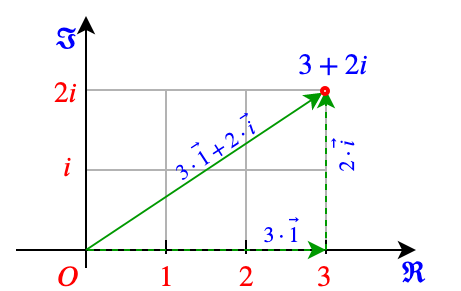
\includegraphics[scale=0.5]{complex.png}
\end{center}
\item Как и прежде, мы умеем отличать на плоскости векторы и точки. Векторы --- это направленные отрезки, которые можно откладывать от точек. Сложение векторо означает их последоватеьлное откладывание. В результате таких откладываний мы уходим от некоторой стартовой точки и приходим в какую-то финишную точку. Результирующий вектор соединяет стартовую и финишную точки. Договоримся для удобства считать стартовой точкой начало координат $O$, а финишную точку обозначать почти так же, как вектор, который в нее входит, только без векторной символики.
\item Итак, если вектор равен $x\vec 1+y\vec i$, то его финишная точка обозначается $x+yi$.
\item Пока все, что мы сделали --- это построили обычную арифметику векторов на плоскости. При чем же тут алгебраическая ипостась мнимой единицы, вытекающая из уравнения $x^2=-1$?
\item Алгебраическая ипостась $i$ нам нужна как раз для того, чтобы построить алгебру точек плоскости, т.е. научиться их не только складывать и умножать на число, но еще и умножать и делить друг на друга.
\item Примем за аксиому, что с числами вида $x+iy$ мы будем обращаться как с обычными числами, пользуясь аксиомами поля, и при этом пользоваться тем самым свойством мнимой единицы, которое ее определяет, т.е. равенством $i^2=1$.
\item Например,
$$
(a+bi)(x+yi) = ax + ayi + bxi + byi^2 = (ax-by) + (ay+bx)i.
$$
\item Числа вида $z=x+iy$ с заданными операциями сложения и умножения (сложение --- покоординатное, а умножение определено выше) называются \textbf{компл\'eксными числами}. При этом $x$ называется \textbf{действительной} (или вещественной) частью комплексного числа $z$ и имеет также обозначение $\Re z$, а $y$ называется \textbf{мнимой} частью числа $z$ и имеет также обозначение $\Im z$.
\item Координатная ось $Ox$ на комплексной плоскости называется действительной осью, а координатная ось $Oy$ --- мнимой.
\item Дадим следующие определения. Число $\bar z=x-yi$ называется \textbf{комплексно сопряженным} к числу $z=x+iy$. Комплексное сопряжение --- это отражение относитеьлно действительной оси.
\item Модулем комплексного числа $z=x+yi$ называется число $$|z|=\sqrt{x^2+y^2}.$$
Нетрудно видеть, что модуль комплексного числа --- это длина соответствующего ему вектора (по теореме Пифагора). Кроме того, из геометрических соображений понятно, что $|z_1-z_2|$ --- это расстояние между точками $z_1$ и $z_2$ на плоскости.
\begin{center}
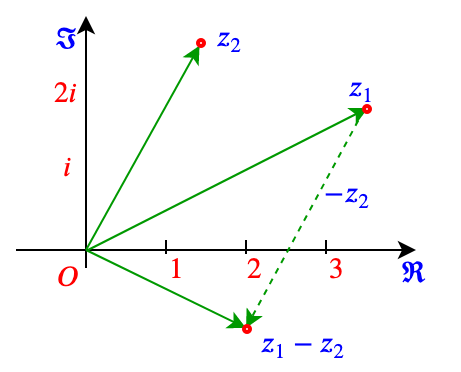
\includegraphics[scale=0.5]{rho.png}
\end{center}
\item Посмотрим, какие арифметические свойства комплексных чисел можно извлечь.
\begin{enumerate}[\bf C1)]
\item $z\bar z=|z|^2$. Действительно, $(x+yi)(x-yi)=x^2+y^2$.
\item $z=0$ (т.е. $z=0+0i$) тогда и только тогда, когда $|z|=0$.
\item Обратное по умножению число для $z\ne 0$ существует и равно
$$
z^{-1} = \frac{1}{x+yi}=\frac{x-yi}{(x+yi)(x-yi)}=\frac{\bar z}{|z|^2}
$$
Это можно получить и напрямую из свойства C1.
\item Мультипликативное свойство сопряжения: $\bar{zw}=\bar{z}\bar{w}$. Действительно,
$$ 
\bar{(x+yi)(a+bi)} = \bar{(ax-by)+(ay+bx)i} = (ax-by)-(ay+bx)i
$$
и
$$
\bar{(x+yi)}\bar{(a+bi)} = (x-yi)(a-bi) = (ax-by)-(ay+bx)i.
$$
\item Мультипликаивное свойство модуля: $|zw|=|z||w|$. Действительно,
$$
|zw|^2 = zw\bar{zw} = zw\bar{z}\bar{w} = z\bar{z}w\bar{w} = |z||w|.
$$
\end{enumerate}
\item Сложение с числом $z=x+iy$ --- это параллельный перенос $T_{\vec z}$ на вектор $\vec z=x\vec 1+y\vec i$. Это следует из геометрических свойств комплексных чисел, о которых мы говорили выше.

Кроме того, это легко проверить арифметически. Пусть даны две точки $z_1$ и $z_2$. Добавим к ним вектор $z$, получим новые точки $z_1'=z_1+z$ и $z_2'=z_2+z$. Во-первых, заметим, что расстояние сохранилось:
$$
|z_1'-z_2'| = |(z_1+z)-(z_2+z)| = |z_1-z_2|,
$$
т.е прибавление $z$ --- это движение. Во-вторых, если $z\ne 0$, то у этого движения нет неподвижных точек, иначе мы бы получили равенство $z_1+z=z_1$, откуда $z=0$. Следовательно, в силу теоремы Шаля прибавление $z$ есть параллельный перенос. Прибавление $z=0$ есть $\id$.
\item Умножение на комплексное число, по модулю равное 1, есть поворот с центром в нуле.

Пусть $|z|=1$. Возьмем точки $w_1=a_1+b_1i$ и $w_2=a_2+b_2i$,  умножим их на $z$, получим точки $w_1'=w_1z$ и $w_2'=w_2z$.

Найдем расстояние между $w_1'$ и $w_1'$:
$$
|w_1'-w_2'|=|(w_1-w_2)z|=|w_1-w_2|\cdot|z|=|w_1-w_2|,
$$
т.е. умножение на $z$ сохраняет расстояние. В то же время, очевидно, что при $z\ne 1$ единственной неподвижной точкой при умножении будет $w=0$, иначе мы бы получили $wz=w$, т.е. $z=w/w=1$. Умножение на $z=1$ есть $\id$.

Итак, умножение на число $z$, по модулю равное 1, является поворотом с центром в нуле. \textit{Каков при этом угол поворота?} 

Чтобы ответить на данный вопрос, рассморим для начала случай $|w|=1$, т.е. точку с единичой окружности будем умножать на другую точку с единичной окружности. По свойствам модуля имеем $|zw|=|z||w|=1$, т.е. в результате умножения мы вновь получим точку на единичной окружности! Иначе говоря, единичная окружность с операцией умножения комплексных чисел образует группу.

Теперь, заметим, что на окружности радиуса 1 хорда однозначно определяет опирающийся на нее угол. Рассмотрим углы, которые опираются на хорду $[z;1]$ и на хорду $[zw;w]$. На рисунке они выделены красным цветом.
\begin{center}
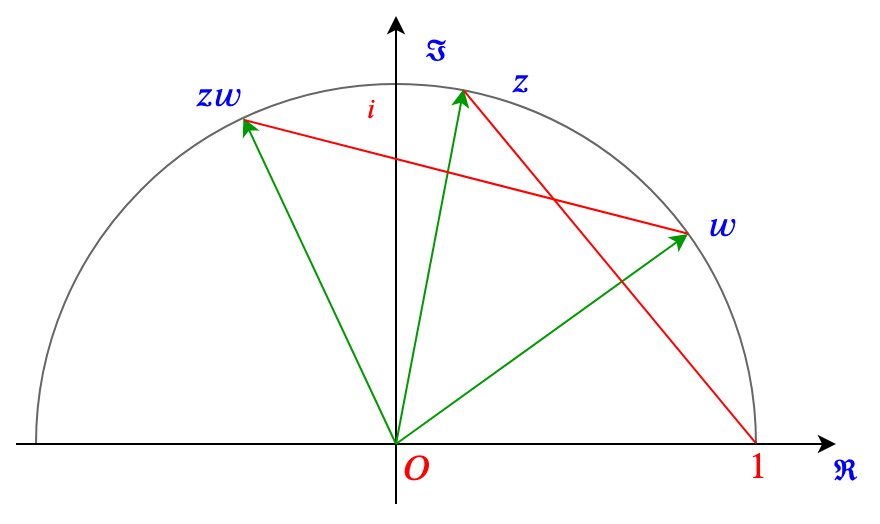
\includegraphics[scale=0.4]{complex-ring.png}
\end{center}

Легко видеть, что длины хорд равны: $|zw-w|=|z-1||w|=|z-1|$, так что и углы равны. Следовательно, точка $zw$ получается из точки $w$ поворотом на угол, соответствующий угу наклона вектора $z$ относительно положительного направления действитеьлной оси.

Что происходит в случае, когда $w$ не лежит на единичной окружности и отлична от нуля? Для этого представим произведение $zw$ следующим образом:
$$
zw = z\frac{w}{|w|}|w|,
$$
где отношение $w/|w|$ уже является комплексным числом единичной длины. Следовательно, число $zw/|w|$ получается из числа $w/|w|$ его поворотом на угол, заданный числом $z$. Осталось выяснить, как связаны $w$ с $w/|w|$ и $zw$ с $zw/|w|$.

В общем случае это означает, что мы имеем два комплексных числа, одно $v$, второе $\la v$, где действительное число $\la>0$. Пусть $v=a+bi$. Вспомним уравнение прямой, проходящей через начало координат и точку $(a,b)$. Это уравнение имеет вид $ay-bx=0$. А теперь умножим в этом уравнении обе части на $\la$, и получим $(\la a)y-(\la b)x=0$. То есть точка $\la v$ лежит на той же прямой, что и $v$.

Остался вопрос --- с одной ли стороны относительно нуля они лежат? Чтобы это проверить, нужно сравнить длину их разности с суммой длин:
$$
|\la v-v|=|v||\la-1|<(1+\la)|v|=|v|+|\la v|,
$$
т.е. да, они лежат на одной прямой по одну сторону от нуля.
\begin{center}
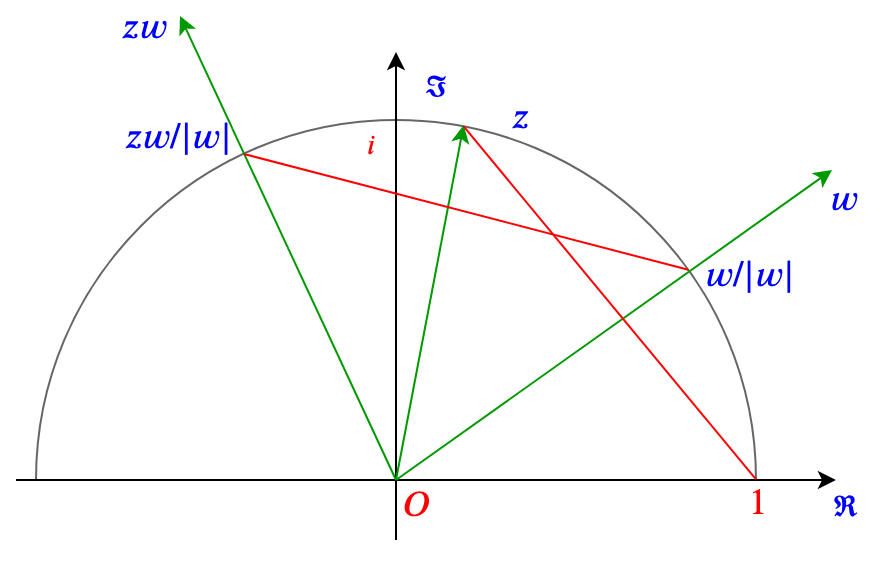
\includegraphics[scale=0.4]{complex-ring2.png}
\end{center}

Итак, число $zw$ получается следующим способом: сначала $w$ переводится на единичную окружность нормировкой, т.е. делением на модуль, получается $w/|w|$. Затем оно поворачивается на угол, заданный числом $z$, затем оно возвращается на свою орбиту, т.е. домножается на $|w|$. В итоге это есть не что иное, как поворот точки $w$ на угол, заданный числом $z$.
\item Кстати, угол, заданный числом $z$, а в общем случае, числом $z/|z|$ (если $z$ --- произвольное ненулевое комплексное число), называется \textbf{аргументом числа} $z$ и обозначается $\arg z$.
\item Основные тригонометрические функции определяются с помощью комплексного числа с единичной окружности так: пусть задан угол $\ph$. Повернем вектор $(1,0)$ на этот угол и найдем число $z$ на единичной окружности такое, что $\arg z=\ph$, тогда
$$
\cos\ph = \Re z,\quad \sin\ph=\Im z.
$$
\item Как уже отмечалось выше, операция комплексного сопряжения есть не что иное как отражение относительно действительной оси. Так что все базовые виды движений плоскости у нас представлены. Учитывая также, что поворот с произвольным центром можно представить как композицию сдвига, поворота с центром в нуле и обратного сдвига, а отражение относительно произвольной оси --- как композицию поворота или сдвига, отражения относительно действитеьлной оси и обратного поворота или сдвига, приходим к тому, что все движения плоскости можно выразить через три изученных нами действия с комплексными числами: сложение (произвольный сдвиг), умножение на число с единичной окружности (поворот с центром в нуле) и сопряжение (отражение относительно действитеьлной оси).
\item На будущее у нас остается вопрос: \textit{какое преобразование плоскости осуществляет умножение на произвольное ненулевое комплексное число?}
\item Поскольку мы пока знакомы только с рациональными дробями, комплексные числа у нас также являются рациональными, т.е. имеют вид $\frac{a}{b}+\frac{c}{d}i$, где $a,b,c,d\in\Z$ и $b,d\ne 0$. Но даже при таком существенном ограничении мы уже имеем дело с еще одним полем --- \textbf{полем комплексных рациональностей}, поскольку сложение, вычитание, умножение и деление не выводит нас за пределы этого множества (единственное исключение --- модуль числа может выпасть из $\Q$). Такое поле обоначается $\Q[i]$ и является расширением поля $\Q$, аналогично полю $\Q[\sqrt 2]$, рассмотренному ранее.
\end{enumerate}

\subsection*{Задачи}

\begin{enumerate}
\item Докажите, что если $\la>0$, то $|\la-1|<\la+1$.
\end{enumerate}


\section{Гауссовы целые числа}

\subsection*{Конспект}

\begin{enumerate}
\item В этом разделе мы ограничимся рассмотрением комплесных чисел с целыми координатами, т.е. чисел вида
$$
a+bi,\quad a,b\in\Z
$$
Легко видеть, что такие числа образуют коммутативное кольцо с единицей. Данное кольцо обозначается $\Z[i]$ и называется кольцом \textbf{гауссовых целых чисел}. На координатной плоскости точки $\Z[i]$ сосредоточены в узлах целочисленной решетки.
\item Число $a+bi$ \textbf{делится на} $c+di$, если существует число $a'+b'i$ такое, что $a+bi=(c+di)(a'+b'i)$. Обозначение аналогично обычному в натуральных числах: $(c+di)|(a+bi)$. Например, число 2 делится на $(1+i)$, т.\,к. $2=(1+i)(1-i)$.

\item 
Нормой гауссова числа $a+bi$ называется величина $$N(a+bi)=(a+bi)(a-bi)=a^2+b^2,$$
т.е. норма числа $z$ равна $z\bar z$

 Несколько свойств нормы:
\begin{enumerate}[{\bf Norm1}]
\item $N(a+bi)=0$ тогда и только тогда, когда $a=b=0$.
\item Нормы комплексно сопряженных чисел совпадают.
\item Если норма нечётна, то она имеет вид $4k+1$, никакая норма не может быть равна $4n+3$.

Поскольку $N(a+bi)=a^2+b^2$, легко видеть, что она является нечетным числом только в том случае, когда $a$ четное, $b$ нечетное, либо наоборот. Пусть $a=2k$, $b=2j+1$, тогда $a^2+b^2=4k^2+4j^2+4j+1 = 1\pmod 4$.

\item $N(zw)=N(z)N(w)$, где $z,w$ --- гауссовы числа.

Пусть $z=a+bi$, $w=c+di$, тогда
\begin{align*}
N(zw)    & = N(ac-bd+i(ad+bc)) = a^2c^2+b^2d^2+a^2d^2+b^2c^2 \\
N(z)N(w) & = (a^2+b^2)(c^2+d^2) = a^2c^2+a^2d^2+b^2c^2+b^2d^2.
\end{align*}
\end{enumerate}
Последнее свойство означает, что  делителями единицы (обратимыми элементами) могут быть только числа с нормой 1, т.\,е. $\pm 1$ и $\pm i$. Других обратимых нет. Геометрически делителями единицы, являются те и только те гауссовы числа, которые лежат на единичной окружности. Отметим также, что все делители единицы образуют множество всех корней 4 степени из 1, т.е. корней уравнения $x^4=1$.

Наконец, множество $\{1,-1,i,-i\}$ является группой по умножению, причем уже хорошо знакомой нам группой, если не обращать внимание на символ операции и символы элементов группы. Сравните таблицы <<умножения двух групп>>: этой и группы сложения вычетов по модулю 4 $\Z_4$:
\begin{center}
\begin{tabular}{c||c|c|c|c|}
* & 1 & i & -1 & -i\\
\hline\hline
1 & 1 & i & -1 & -i\\ \hline
i & i & -1 & -i & 1 \\ \hline
-1 & -1 & -i & 1 & i \\ \hline
-i & -i & 1 & i & -1 \\ \hline
\end{tabular}
\qquad
\begin{tabular}{c||c|c|c|c|}
$+$ &0 & 1 & 2 & 3\\
\hline\hline
0 &0 & 1 & 2 & 3\\ \hline
1 &1 & 2 & 3 & 0 \\ \hline
2 &2 & 3 & 0 & 1 \\ \hline
3 &3 & 0 & 1 & 2\\ \hline
\end{tabular}
\end{center}

Если произвести соответствие $1\mapsto 0$, $i\mapsto 1$, $-1\mapsto 2$, $-i\mapsto 3$, а операции умножения поставить в соответствие операцию сложения по модулю 4, то мы получим и полное соответствие между результатами умножения в первой группе и сложения во второй: $i(-1)\mapsto 1+2$ и т.д.

В том случае, когда можно предъявить взаимно однозначное соответствие элементов двух групп так, чтобы операция в первой группе соответствовала операции во второй, говорят о том, что эти две группы \textbf{изоморфны}. Очень часто такие группы даже считают равными, хотя природа у них разная. Итак, группа по умножению обратимых гауссовых чисел изоморфна группе $\Z_4$.


\item Все гауссовы числа делятся на делители единицы. Это легко понять из групповых свойств делителей единицы. Действительно, разделить на 1 означает умножить на нее, т.к. 1 сама себе обратна по умножению. Разделить на $i$ означает умножить на $-i$, т.к. эти числа взаимно обратны по умножени. Аналогично, разделить на $-1$ означает умножить на -1, и разделить на $-i$ означает умножить на $i$.

\item Делители единицы обладают еще одним замечательным свойством: умножение на них --- это поворот относительно начала координат, причем умножение на $i$ есть поворот на угол $\pi/2$, умножение на -1 --- поворот на угол $\pi$ (т.е. центральная симметрия), умножение на $-i$ --- поворот на угол $3\pi/2$ или $-\pi/2$. То есть делители единицы соответствуют еще и группе вращений квадрата.


\item Два гауссовых числа называют \textbf{ассоциированными}, если одно получается из другого умножением на делитель единицы. Ассоциированность является отношением эквивалентности, причем каждый класс эквивалентности включает ровно 4 числа, расположенных в углах квадрата с центром в 0. Например, $1+2i$, $-2+i$, $-1-2i$ и $2-i$ ассоциированы.
\begin{center}
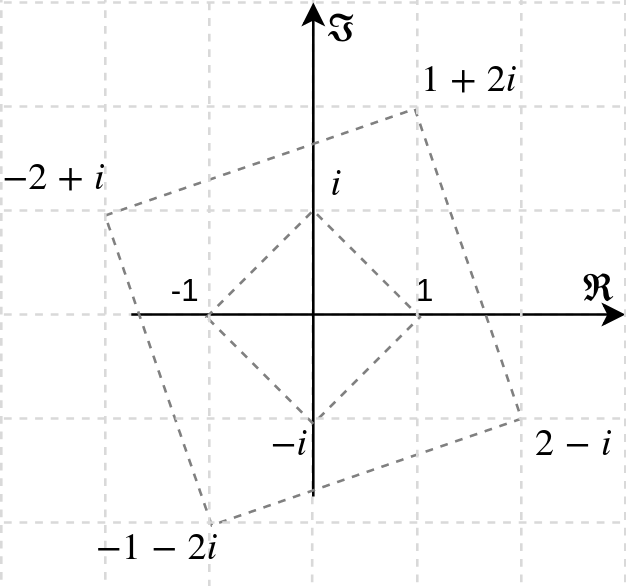
\includegraphics[scale=0.35]{Gaussian.png}
\end{center}

\item Свойства делимости гауссовых чисел очень похожи на таковые свойства в арифметике натуральных чисел, но есть и отличия.
Приведем несколько свойств:
\begin{enumerate}[\bf\hbox{Div}1]
\item Если гауссово число $a+bi$ делится на обычное целое число $c+i0$, то $c|a$ и $c|b$ в целых числах.

Это легко видеть из равенства $a+bi=(x+yi)(c+i0)=xc+yci$, откуда $a=xc$ и $b=yc$.
\item Если $z|w$ и $w|z$, то $z$ и $w$ ассоциированы.

Пусть $w=z'z$ и $z=w'w$, откуда $N(w)=N(z')N(z)$ и $N(z)=N(w')N(w)$, откуда $N(z')N(w')=1$ и, следовательно, $N(z')=N(w')=1$, поскольку в натуральных числах это единственное решение. Стало быть, $z'$ и $w'$ --- делители единицы.

\item Ассоциированность сохраняет делимость: если $z$ и $w$ ассоциированы, $u$ и $v$ ассоциированы, то $(z|u)\to (w|v)$.

Действительно, пусть $z=z'w$ и $u=u'v$, где $z',u'$ --- делители единицы. Тогда
$$
\frac{u}{z} = \frac{u'}{z'}\frac{w}{v},
$$
так что если отношение $u/z$ является гауссовым числом, то отношение $v/w$ является ассоциированным с ним числом.
\item $z$ ($N(z)>1$) имеет как минимум 8 делителей: своих ассоциированных и ассоциированных с 1.
\item Делители $z$ являются делителями $N(z)$, если $N(z)$ рассматривать как гауссово число.

Пусть $w|z$, т.е. $z=uw$. Поскольку $N(z)=z\bar z=w(u\bar z)$, очевидно, что $N(z)$ делится на $w$.
\item Норма $z=a+bi$ четна тогда и только тогда, когда $(1+i)|z$, в частности, если $a$ и $b$ имеют разную четность, то $z$ не делится на $1+i$.

Для начала заметим, что норма $z=a+bi$ четна тогда и только тогда, когда $a$ и $b$ имеют одинаковую четность, т.е. сравнимы по модулю 2. Далее, поскольку $(1+i)|z$, существует $c+di$ такое, что
$$
a+bi = (1+i)(c+di) = c-d + i(c+d),
$$
т.е. $a=c-d$, $b=c+d$, что равносильно $a-b=-2d$, $a+b=2c$ при некоторых $с,d\in\Z$, а это равносильно тому, что $a\equiv b\pmod 2$.
\end{enumerate}

\item В кольце $\Z[i]$ можно любое число $u$ разделить на любое число $v\ne 0$ с остатком, так что получится
\begin{equation}\label{Ostat}
u=qv+r,\quad N(r)<N(v).
\end{equation}
При этом выбор чисел $q$ и $r$ можно строго ограничить, выбирая $q$ как ближайшее гауссово число к комплексному $u/v\in\Q[i]$, а $r$ как разность между $u$ и $qv$. В случае, когда выбор $q$ неоднозначен (может быть максимум 4 числа), можно договориться выбирать то, которое на координатной сетке находится левее и/или ниже.

Приведем один из вариантов вычисления $r$. Пусть $u=a+bi$ и $v=c+di$. Далее оперируем в поле $\Q[i]$:
$$
\frac{a+bi}{c+di}=\frac{(ac+bd)+(bc-ad)i}{c^2+d^2}=q_1+\frac{r_1}{c^2+d^2}+q_2i+\frac{r_2}{c^2+d^2}i,
$$
где $ac+bd=q_1(c^2+d^2)+r_1$ и $bc-ad=q_2(c^2+d^2)+r_2$. Здесь мы воспользовались делением с остатком в кольце $\Z$. При этом мы выбираем знаки $r_1$ и $r_2$ так, чтобы выполнялись неравенства:
$$
|r_1|,|r_2|\le (c^2+d^2)/2.
$$
Это всегда возможно, поскольку остатки от деления можно выбирать не только из ряда $0,1,2,\dots,c^2+d^2-1$, но также из ряда
$0,\pm 1,\pm 2,\dots,\pm k$, где $k$ --- целая часть от деления $c^2+d^2$ на 2, так что всегда $k\le(c^2+d^2)/2$. Здесь как раз и может оказаться вплоть до 4-х вариантов выбора.

Тогда
$$
u=(q_1+q_2i)v+\frac{(r_1+r_2i)(c+di)}{c^2+d^2}=(r_1+r_2i)\frac{v}{N(v)},
$$
эту последнюю дробь мы и выберем в качестве остатка $r$.

При этом заметим, что поскольку разность $u-(q_1+q_2i)v$ является гауссовым числом, то таковым же будет и число $(r_1/N(v)+r_2i/N(v))v$, хоть оно и выглядит нецелым.

Далее,
$$
N\left(\frac{r_1}{N(v)}+\frac{r_2}{N(v)}i\right)=\frac{r_1^2+r_2^2}{(c^2+d^2)^2}\le \frac 12,
$$
откуда $N(r)\le (1/2)N(v)<N(v)$.

\item На основе деления с остатком нетрудно получить выполнимость алгоритма Евклида (см. раздел \ref{EVKL}) для гауссовых чисел:
\begin{align*}
u & = q_1v + r_1, &  N(r_1)<N(v),\\
v & = q_2r_1 + r_2, &  N(r_2)<N(r_1),\\
r_1 & = q_3r_2 + r_3, &  N(r_3)<N(r_2),\\
\dots & \dots & \\
r_{n-1} = q_{n+1}r_n + r_{n+1}, &  N(r_{n+1})<N(r_n),\\
r_{n} = q_{n+2}r_{n+1}, &  N(r_{n+1})<N(r_n),\\
\end{align*}
поскольку норма является натуралным числом и не может убывать бесконечно.

Отсюда так же, как для целых чисел, выводится и представление $\gcd(u,v)$ в виде линейной комбинации исходных чисел $u,v$. Но мы докажем этот факт иным способом.
\begin{lem}\label{NOD}
Для любых гауссовых чисел $u,v\ne 0$ существует гауссово число $r$ такое, что:

\textup{1)} $r|u$ и $r|v$ (общий делитель);

\textup{2)} если $(q|u)\wedge(q|v)$, то $q|r$ (наибольший общий делитель);

\textup{3)} существуют гауссовы $x,y$ такие, что $r=xu+yv$.

\noindent Кроме того,

\textup{4)} число $r$, удовлетворяющее \textup{1)--3)}, единственное с точностью до ассоциированности.
\end{lem}
\pf
Рассмотрим множество $R(u,v)=\{xu+yv|\;x,y\in\Z[i]\}\setminus\{0\}$. В множестве норм $\{N(z)|\;z\in R(u,v)\}$ существует наименьшее положительное число (т.\,к. нуля там быть не может). Пусть $r\in R(u,v)$ такое число, у которого норма минимальная (оно может быть не единственное, выберем одно). Остается показать, что $r$ --- искомое.

Во-первых, $r$ имеет вид $xu+yv$ по построению, т.е. выполняется пункт 3). Во-вторых, если $(q|u)$ и $(q|v)$, то очевидно, что $q|r$ также по построению $r$, т.е. выполняется пункт 2).

Докажем пункт 1).
Из \eqref{Ostat} имеем: $u=rt+s$, где $N(s)<N(r)$. Подставляя представление $r$, имеем:
$u=xut+yvt+s$, откуда $s=(1-xt)u+(-yt)v$. Если $s\ne 0$, то $s\in R$ как линейная комбинация $u$ и $v$, но тогда $N(s)\ge N(r)$ в силу выбора $r$, а это не так в силу \eqref{Ostat}. Следовательно, $s=0$, откуда $r|u$. Аналогично, $r|v$.

Докажем пункт 4). Пусть $r'=x'u+y'v$ также удовлетворяет свойствам 1)--3). Тогда $r|r'$ и $r'|r$. Из первого следует, что $r'=rt$ и $N(r')=N(r)N(t)$, из второго следует, что $r=r't'$ и $N(r)=N(r')N(t')$. Таким образом, нормы $N(t)$ и $N(t')$ взаимно обратны в натуральных числах, откуда следует $N(t)=N(t')=1$, т.\,е. $t$ --- делитель 1 и, следовательно, $r$ и $r'$ ассоциированы.
\epf

\item Доказанная лемма позволяет определить понятие НОД для гауссовых чисел с точностью до ассоциированности. В качестве НОД мы будем выбирать какое-то одно из четырех (наиболее удобного вида).

\item Гауссово число называется \textbf{простым}, если оно не имеет никаких делителей, кроме тривиальных (ассоциированных с 1 и самим собой), и не является делителем 1, т.\,е. простое гауссово число имеет ровно 8 делителей. Два гауссовых числа называются \textbf{взаимно простыми} (обозначается $u\perp v$), если их НОД --- обратимое число, т.\,е. 1 и ассоциированные с ней.

\item Верны следующие свойства простых гауссовых чисел:
\begin{enumerate}[\bf\hbox{Prim}1]
\item Если $a+bi$ простое, то $a-bi$ также простое.

Действательно, если $a-bi=uv$, где $u,v$ не ассоциированы с 1, то $a+bi=\bar u\bar v$, где $\bar u$ и $\bar v$ не ассоциированы  с 1 (т.к. для делителей нуля сопряжение не нарушает ассоциированности), нотогда $a+bi$ не является простым.
\item Если $z$ простое, то его ассоциированные также простые.
\item Если $z$ простое и $z|uv$, то $(z|u)\vee(z|v)$;

Действительно. Пусть простое $z|uv$. Предположим, что $\neg(z|u)$, тогда $z\perp u$, откуда по лемме \ref{NOD} получаем, что $1=xz+yu$. Умножаем на $v$: $v=xzv+yuv$. Справа оба слагаемых делятся на $z$, следовательно, $z|v$. Аналогично, если $\neg(z|v)$, то $z|u$.

\item Норма простого, неассоциированного с $1+i$, всегда нечетна, т.\,е. имеет вид $4k+1$.

Это следует из свойства Div6. Если простое число не ассоциировано с $1+i$, то оно и не делится на него, а значит, по свойству Div6 его норма нечетная. То, что она имеет вид $4k+1$, следут из $(2k)^2+(2n+1)^2=4m+1$.
\item Натуральное простое не всегда есть гауссово простое: $5=(2+i)(2-i)$.
\item \textbf{Критерий Гаусса}:
\begin{thrm}
$a+bi$ простое тогда и только тогда, когда\\
\textup{1)} либо одно из чисел $a,b$ нулевое, а второе --- простое целое число вида $\pm(4k+3)$ ($k>0$), \\
\textup{2)} либо $a,b$ ненулевые и норма $N(a+bi)=a^2+b^2$ --- простое натуральное число.
\end{thrm}
\item \textbf{Следствие}: простое натуральное вида $4k+1$ не может быть простым гауссовым, простые натуральные вида $4k+3$ являются простыми гауссовыми.
\item Простое натуральное $4k+1$ можно представить как сумму квадратов $a^2+b^2$ (\textbf{рождественская теорема Ферма}).
\item Если $N(z)\perp N(w)$ в натуральных числах, то $z\perp w$ в гауссовых числах.

Пусть $u=\gcd(z,w)$ в гауссовых числах. Тогда $z=ut$, $w=ut'$ и $N(z)=N(u)N(t)$, $N(w)=N(u)N(t')$. Откуда $N(u)|N(z)$ и $N(u)|N(w)$. Тогда из условия $N(z)\perp N(w)$ следует, что $N(u)=1$, т.\,е. $u$ --- ассоциированное с 1 гауссово число. Откуда $z\perp w$.
\end{enumerate}
Примеры простых гауссовых чисел: $\pm 3, \pm 7, \pm 3i$; $1\pm i, 1\pm 2i, 1\pm 4i$.

\item Для гауссовых чисел существует аналог основной теоремы арифметики (см. раздел \ref{PrimeNumbers}):
\begin{thrm}[Основная теорема арифметики гауссовых чисел]\label{OTAG}\quad\\
Каждое ненулевое неассоциированное с 1 гауссово число раскладывается на гауссовы простые множители, причем это разложение единственно с точностью до ассоциированных с этими множителями простых и порядка множителей, т.\,е. разложение имеет вид
$$
\al_1^{s_1}\dots \al_n^{s_n}=\be_1^{s_1}\dots \be_n^{s_n},
$$
где пары $\al_i,\be_i$ являются ассоциированными простыми числами, а степени $s_i$ --- натуральными числами.
\end{thrm}
Доказательство теоремы прямо следует из свойства Prim3.

Пример: $5=(2+i)(2-i)=(1+2i)(1-2i)$ (множители переводятся друг в друга умножением на $i$ и на $-i$).

\item Из ОТА легко выводится следующее утверждение
\begin{lem}\label{OLF}
Если $(u\perp v)\land(uv=c^n)$, то существуют $a\perp b$ такие, что $u=a^n$ и $v=b^n$ и $c=ab$.
\end{lem}


Заметим, что и в обычной арифметике целых чисел верна такая же лемма. Более того, как основная теорема арифметики \ref{OTAG}, так и лемма \ref{OLF} верны в любом \textbf{евклидовом кольце} (т.\,е. в таком кольце, где возможно деление с остатком в виде \eqref{Ostat} при некоторой натурально-значной норме и, как следствие, алгоритм Евклида). Этим свойством евклидовых колец мы еще воспользуемся в дальнейшем.

\item Рассмотрим парочку примеров, где числа Гаусса дают заметный выигрыш по скорости и простоте решения задач, связанных с уравнениями в целых числах, т.е. \textbf{диофантовыми уравнениями}.
\item Рассмотрим уравнение $$x^2+1=y^3,\quad x,y\in\Z.$$
В гауссовых числах оно эквивалентно уравнению $$(x+i)(x-i)=y^3.$$

\item Покажем, что $x+i\perp x-i$. Действительно, если это не так, т.\,е. $z|x+i$ и $z|x-i$, то $z|(x+i)-(x-i)=2i$, откуда $z=1+i$ или ему ассоциированное. Кроме того, $z|y^3$, причем, поскольку $1+i$ --- простое, оно должно входить в разложение $y^3$ трижды, т.\,е. $z^3|y^3$, но тогда в разложение $x+i$ или $x-i$ входит $z^2=2i$, чего быть не может, т.\,к. $x\pm i$ не делится на 2 (см. свойство Div1). Следовательно, $x+i\perp x-i$.

\item Из предыдущего и леммы \ref{OLF} следует, что существует число $a+bi$ такое, что $x+i=(a+bi)^3$. Возводя в куб и сравнивая коэффициенты при $i$, находим, что $1=b(a^2-b^2)$. Это --- уравнение в целых числах, поэтому $b=\pm 1$, откуда $a^2=0$ или 2. Но $a^2=2$ неразрешимо в целых числах, поэтому $a=0$, откуда $x=0$. Таким образом, единственно возможное решение в целых числах у исходного уравнения $x^2+1=y^3$ --- это $x=0, y=1$.

\item Рассмотрим \textbf{Теорему Ферма} при $n=2$: $a^2+b^2=c^2$ (в натуральных числах). Ясно, что можно сразу считать, что все числа $a,b,c$ попарно взаимно простые натуральные числа (иначе можно было бы сократить уравнение на общий множитель). Отсюда также следует, что $a$ и $b$ имеют разную четность. Действительно, если $a$ и $b$ четные, то таково же и $c$, а значит, они не взаимно простые. Если $a$ и $b$ нечетные, то $a^2+b^2$ имеет остаток 2 при делении на 4, но $c^2$ может иметь остаток либо 0 (четное), либо 1 (нечетное). Таким образом, допускается только случай, когда $a$ и $b$ имеют различную четность. Тогда по свойству Div6 число $a+bi$ не делится на $1+i$.

\item Заметим, что $(a+bi)(a-bi)=a^2+b^2=c^2$. Предположим, что НОД чисел $a+bi$ и $a-bi$ равен $r$ и отличен от делителя 1. Тогда $r|2a$ и $r|2bi$. Но $a\perp b$ в натуральных числах, тогда $N(a)\perp N(b)$, откуда по свойству Prim9 $a\perp b$ в гауссовых числах. Это значит, что $r$ есть НОД 2 и $2i$, т.\,е. $r=1+i$ или его ассоциированным. Но такое число не может быть делителем $a+bi$ и $a-bi$ по доказанному выше. Следовательно, $(a+bi)\perp (a-bi)$.

\item Тогда по лемме \ref{OLF} существуют такие $z,w$, что $a+bi=z^2$, $a-bi=w^2$ и $c=zw$. Пусть $z=n+mi$, тогда $a+bi=n^2-m^2+2nmi$, откуда $a-bi=n^2-m^2-2nmi$, откуда $w=n-mi$ и $c=n^2+m^2$.

\item Таким образом, мы получаем формулу \textbf{пифагоровых троек}:
$$
a=n^2-m^2,\quad b=2nm,\quad c=n^2+m^2,
$$
где натуральные $n,m>0$.

\item Рассмотрим теперь уравнение $x^4+y^4=z^4$, неразрешимость которого доказал еще сам Ферма методом, который мы покажем ниже. 

\item Докажем более сильное утверждение: $x^4+y^4=z^2$ неразрешимо в целых положительных числах.
\item Как и прежде, считаем сразу же, что $x\perp y$. Посмотрим на это уравнение как на уравнение второй степени: $(x^2)^2+(y^2)^2=z^2$. Если оно разрешимо, то существуют ненулевые взаимно простые $n,m$ такие, что
$$
x^2=n^2-m^2,\quad y^2=2nm,\quad z=n^2+m^2,
$$
откуда вновь получаем уравнение второй степени $x^2+m^2=n^2$, а значит, его решение имеет вид:
$$
x=a^2+b^2,\quad m=2ab,\quad n=a^2+b^2,
$$
где ненулевые $a\perp b$. Тогда для $y$ имеет место равенство: $y^2=4nab$ и, поскольку число 2 простое (в обычных целых числах), $y=2y'$.

Тогда $(y')^2=nab$. Так как $n,a,b$ попарно взаимно просты (это следует из того, что $a\perp b$ и $n=a^2+b^2$), в силу леммы \ref{OLF} (для обычных целых чисел) существуют такие $s,t,k$, что $n=s^2$, $a=t^2$, $b=k^2$. Подставляем это в равенство $n=a^2+b^2$, получаем:
$$
t^4+k^4=s^2,
$$
где $t\perp k$ и $z>s>0$ (это следует из того, что $s=\sqrt n$, $n^2<z$). 

Таким образом, имея одно решение $(x,y,z)$ исходного уравнения, мы построили еще одно $(t,k,s)$, где $s<z$. Продолжая применять эти построения далее, мы получим бесконечную последовательность решений $(t_j,k_j,s_j)$ такую, что $z>s>s_1>s_2>\dots$ Но это невозможно, т.\,к. в натуральном ряде не существует бесконечная строго убывающая последовательность.

\item Полученное противоречие доказывает неразрешимость уравнения $x^4+y^4=z^2$ в целых положительных числах, а значит, и неразрешимость уравнения $x^4+y^4=z^4$. Заметим, что отсюда сразу же следует справедливость теоремы Ферма для всех степеней $n$, кратных 4.

\item Предъявленный здесь метод доказательства называется \textbf{методом бесконечного спуска}. Он напоминает индукцию, только не доказующую, а опровергающую, поскольку приводит к противоречию.

\end{enumerate}



\subsection*{Задачи}





\chapter{Некоторые иррациональности}

\vrezka{
В этой главе мы заглянем за пределы поля рациональных чисел при помощи многочленов с рациональными коэффициентами, построим поле алгебраических чисел, разберем некоторые теоремы о многочленах над кольцами и полями.
}

\section{*Упорядоченные множества}\label{Ordering}

\subsection*{Конспект}

\begin{enumerate}
\item Ранее мы определяли \textbf{отношение на множестве} $A$ как произвольное подмножество $R\subseteq A\times A$.
\item Рассмотрим здесь частный случай отношений: \textbf{отношения порядка}.
\item Вспоминая изучение движений прямой, скажем, что точка $X$ на прямой \textbf{больше}, чем точка $Y$, если $X$ находится правее, чем $Y$. Иначе это можно сформулировать так: если $X=T_a(Y)$, где $a$ --- вектор движения вправо, т.е. положительный вектор. То есть, $X>Y$ (или $Y<X$), если $X$ получается смещением $Y$ в положительном направлении.
\item Симметрично рассуждая, получаем, что $X<Y$, если $X$ находится левее $Y$, либо если из точки $Y$ можно попасть в $X$ сдвигом влево.
\item Пользуясь этим наглядным представлением, легко получить следующие свойства сравнения:
\begin{enumerate}[{\bf Rel1}]
\item если $X<Y$ и $Y<Z$, то $X<Z$ (транзитивность отношения $<$);

Это достаточно очевидно, поскольку сдвиг $T_{XZ}$ есть композиция положительных сдвигов $T_{XY}$ и $T_{YZ}$.
\item для любой точки $X$ не верно, что $X<X$ (антирефлексивность);

Это также довольно-таки очевидно, т.к. сдвиг, сотавляющий на месте $X$, является $\id$, а не положительным сдвигом.
\item для любых точек $X,Y$ имеет место одно из трех отношений: $X<Y$ или $X=Y$ или $X>Y$ (связность).

Это следует из того, что если $X\ne Y$, то можно построить вектор $\vec{XY}$, а он может смотреть либо влево, либо в право, что и будет соответствовать оставшимся двум сравнениям. Заметим сразу, что для любой пары точек всегда выполняется только одно из трех отношений, поскольку равенство $X=Y$ исключает неравенства $X<Y$ и $Y<X$ в силу свойства антирефлексивности, а неравенство $X<Y$ исключает неравенство $Y<X$, т.к. иначе по свойству транзитивности мы бы получили $X<X$, что противоречит антирефлексивности.
\end{enumerate}
\item Транзитивное антирефлексивное связное отношение на множестве называется \textbf{линейным порядком}, а само множество, на котором задан линейный порядок, называется \textbf{линейно упорядоченным}.

\item Ранее мы уже определяли отношение эквивалентности как рефлексивное транзитивное симметричное отношение (см. раздел\ref{Rels}). Ниже представлена графическая схема того, из каких понятий формируются отношение эквивалентности и линейного порядка.
\begin{center}
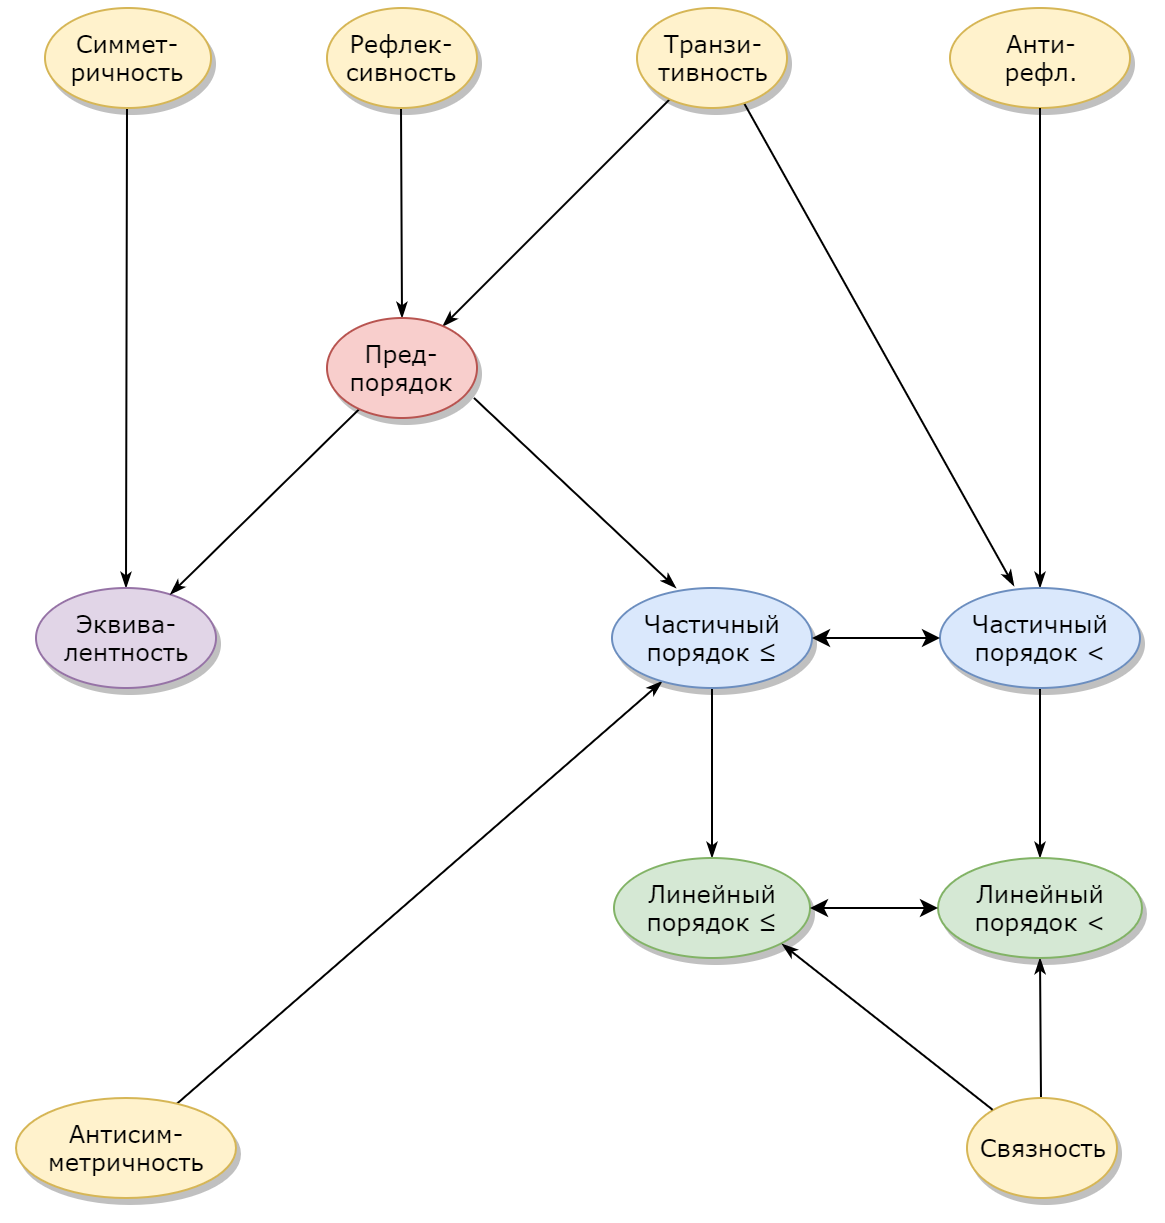
\includegraphics[scale=0.4]{RelOrder.png}
\end{center}

Обратим внимание на то, что отношение линейного порядка здесь представленов двх ипостасях: как антирефлексивное транзитивное и связное отношение, а также как рефлексивное антисимметричное транзитивное и связное оношение. Первый случай соответствует отношению строгого порядка ($<$), второй --- нестрогого ($\le$). Можно доказать, что это на самом деле одно и то же с точностью до исключения равенства.

\begin{lem} Отношение $<$ является отношением строгого линейного порядка тогда и только тогда, когда отношение $\le$ ($(x\le y)\Leftrightarrow (x<y)\lor (x=y)$) является отношением нестрогого линейного порядка.
\end{lem}

В дальнейшем под термином <<линейный порядок>> мы будем понимать именно строгий линейный порядок, а нестрогим будем делать его, используя знак $\le$ и ему подобные.

\item Множества $\N$ и $\Z$ упорядочены естественным образом: числа, стоящие правее, больше, чем их левые собратья.
\item Множество $\Q$ мы, на самом деле, упорядочили еще во время его построения, когда говорили о наклоне прямой, задающей рациональное число: чем круче наклон, тем больше число. Но это верно только для положительных дробей. С отрицательными числами все наоборот (в полной аналогии с целыми числами!) --- чем круче наклон, тем меньше число.
\item Это же можно записать и более формально: если $b>0$ и $d>0$, то
$$
\frac{a}{b}<\frac{c}{d}\Leftrightarrow ad<bc
$$
\begin{center}
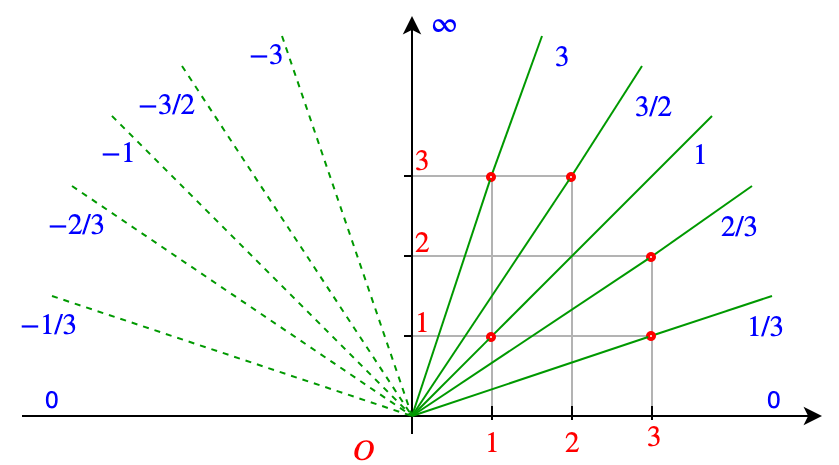
\includegraphics[scale=0.3]{ratio.png}
\end{center}
\item Если на множестве $L$ задан линейный порядок $<$, то \textbf{интервалом} $(x;y)$ называется множество всех точек множества $L$, лежащих между $x$ и $y$:
$$
(x;y) = \{z\in A\mid x<z<y\}
$$
В частности, если $x>y$, то интервал $(x;y)$ пуст. На множестве $\Z$ имеем следующие примеры:
$$
(0;1) = \emptyset,\quad (0;2) = \{1\}, \quad (0;n+1) = \{1,2,\dots, n\}.
$$
\item Линейный порядок $<$ называется \textbf{плотным}, если между любыми двумя элементами всегда есть третий: 
$$
\forall x,y\in L\;(x<y)\to\exists z\; (x<z<y),
$$
т.е. когда любой интервал $(x;y)$ непуст при условии, что $x<y$.
\item Линейно упорядоченное множество с плотным линейным порядком называется \textbf{плотным линейно упорядоченным множеством}.
\item Подмножества линейно упорядоченного множества можно сравнивать. Пусть множество $L$ линейно упорядочено отношением $<$, тогда для его подмножеств $X,Y\subseteq L$ положим
$$
X<Y\Leftrightarrow \forall x\forall y\;(x\in X)\land(y\in Y)\to (x<y),
$$
т.е. когда все точки множества $X$ меньше всех точек множества $Y$.
\item Нетрудно проверить, что отношение $<$ на подмножествах $L$ транзитивно и антирефлексивно. Однако же легко привести пример, когда множества могут быть несравнимы между собой, например, в качестве  $X$ взять все четные числа, а в качестве $Y$ --- все нечетные числа. несмотря на то, что эти множества не пересекаются, невозможно сказать, что $X<Y$ или что $Y<X$, и уж тем более неверно $X=Y$. Таким образом, отношение $<$, определенное на подмножествах $L$ не является линейным порядком.
\item Про отношение, которое является транзитивным и анотирефлексивным, говорят, что оно является \textbf{частичным порядком}.
\item Если множество снабжено частичным порядком, то оно называется \textbf{частично упорядоченным множеством}.
\item Сравнения множеств, как и операции Минковского над ними, удобны тем, что сокращают длинные формальные выкладки, а кроме того, образно очень хорошо воспринимаются: одно множество меньше другого, если оно целиком лежит левее другого.

\item Пусть $(L,<)$ --- линейно упорядоченное множество и $A,B\subset L$, причем $A\ne\emptyset$, $B\ne\emptyset$, $A\cap B=\emptyset$, $A\cup B=L$, $A\le B$\footnote{Здесь и далее сравнение множеств означает сравнение их элементов с квантором всеобщности: $X\le Y$ ($X<Y$) означает, что $\forall x \in X\;\forall y\in Y:\; x\le y$ ($x<y$). То же относится к сравнению множества и элемента: $c\le Y$.}. Тогда пара $(A,B)$ называется \textbf{сечением}\index{Сечение л.у.м.} множества $L$, $A$ --- нижним классом сечения, $B$ --- верхним классом сечения.

\item Линейный порядок $<$ на множестве $L$ называется \textbf{непрерывным}\index{Порядок!линейный!непрерывный} (множество $L$ с таким порядком непрерывно), если каково бы ни было его сечение, либо в нижнем классе сечения существует наибольший элемент, а в верхнем нет наименьшего, либо в верхнем классе существует наименьший элемент, а в нижнем нет наибольшего (такие сечения называются \textbf{дедекиндовыми}).\index{Сечение л.у.м.!дедекиндово} Такое свойство линейного порядка еще называется \textbf{аксиомой непрерывности} или аксиомой полноты.\index{Аксиома!непрерывности (полноты)}

\item Отметим, что плотное линейно упорядоченное множество не всегда непрерывно. Например, $\Q$ плотно, но не непрерывно (сечение для $\sqrt 2$ не является дедекиндовым).\footnote{ВНИМАНИЕ! Термин <<дедекиндово сечение>> в разных источниках определяется по-разному, хотя все эти определения эквивалентны. Часто в качестве сечения берется не пара множеств, а только нижний класс сечения.}

\item Завершим этот раздел соединением двух разнородных понятий: алгебраической структуры и отношения.
\item Пусть имеется числовая структура с операциями $+$ (сложение) и $\cdot$ (умножение), причем символ 0 обозначает в ней нейтральный элемент по сложению. Пусть также на этой структуре задано отношение $<$ линейного порядка. Говорят, что \textbf{отношение $<$ согласовано с операцией $+$}, если выполнено условие:
\begin{enumerate}[resume*]
\item Если $a\le b$, то $a+c\le b+c$ (и $c+a\le c+b$) для любых чисел $a,b,c$ из данной структуры.
\end{enumerate}
Говорят, что \textbf{отношение $<$ согласовано с операцией $\cdot$}, если выполнено условие:
\begin{enumerate}[resume*]
\item Если $a\ge 0$ и $b\ge 0$, то $ab\ge 0$.
\end{enumerate}

Соответственно, если на элементах группы $(G,+)$ задан линейный порядок $<$, согласованный с групповой операцией, то структура $(G,+,<)$ называется \textbf{линейно упорядоченной группой}. Пример такой группы --- группа целых чисел по сложению с обычным порядком.

Если на элементах кольца $(K,+,\cdot)$ задан линейный порядок, согласованный с операциями кольца, то структура $(K,+,\cdot,<)$ называется \textbf{упорядоченным кольцом}. Пример такого кольца --- кольцо целых чисел с обычным порядком.

Наконец, если на элементах поля задан линейный порядок, согласованный с его операциями, то такая структура называется \textbf{упорядоченным полем}. Пример такого поля --- поле рациональных чисел с обычным порядком.

Безусловно, самым <<продвинутым>> для нас на текущий момент понятием является \textit{непрерывное упорядоченное поле}, т.е. поле с непрерывным линейным порядком, согласованным с операциями сложения и умножения. Именно построение такого уникального поля является основной целью нашего курса.
\end{enumerate}

\subsection*{Задачи}

\begin{enumerate}
\item Пусть множество $X$ не пусто. Верно ли, что $\emptyset<X$? Верно ли, что $X<\emptyset$? Верно ли, что $\emptyset<\emptyset$?
\item Каким отношением (антирефлексивным, транзитивным, связным) является отношение несобственного вложения множеств? $X$ есть несобственное подмножество $Y$ (обозначение: $X\subset Y$), если $X\subseteq Y$ и $X\ne Y$.
\item Каким отношением является отношение делимости $x|y$ на положительных целых числах?
\item Является ли всюду плотным множество всех десятично рациональных чисел, т.е. чисел вида $k/10^n$, где $k\in \Z$ и $n\in\N$?
\item Выпишите полный список аксиом упорядоченного поля.
\end{enumerate}


\section{Плотные множества}

\subsection*{Конспект}

\begin{enumerate}
\item Вернемся к анализу поля рациональных чисел $\Q$. Данное поле интересно тем, что какие бы два различных числа мы ни взяли, между ними всегда найдется третье рациональное число. Действительно, пусть есть две дроби $r=n/m$ и $q=t/s$, тогда их среднее арифметическое $(r+q)/2$ является рациональным числом и лежит строго между ними.
\item Таким образом, множество рациональных чисел с обычным отношением сравнения является плотным линейно упорядоченным множеством.
\item К определению понятия плотного множества существует и другой, топологический подход. Пусть $A\subseteq B$, где $B$ --- линейно упорядоченное множество. Говорят, что множество $A$ \textbf{плотно в} $B$, если любой непустой интервал множества $B$ содержит точки $A$. Иначе говоря, как бы мы ни старались выбрать как можно более маленький (но непустой) интервал множества $B$, в нем всегда будут сидеть и точки множества $A$.
\item Можно взять, например, множество $\B\subseteq\Q$ всех двоичных рациональностей, т.е. дробей вида $k/2^n$, где $k\in\Z$, $n\in\N$. Такое множество, во-первых, является плотным, поскольку среднее арифметическое любых двух его представителей
$$
\left(\frac{k}{2^n}+\frac{l}{2^m}\right)/2 = \frac{k\cdot 2^{\max(n,m)-n}+l\cdot 2^{\max(n,m)-m}}{2^{\max(n,m)+1}}
$$
является двоично-рациональным числом.
\item А во-вторых, множество $\B$ плотно в $\Q$, поскольку каковы бы ни были два рациональных числа $r\ne q$, между ними найдется двоично-рациональное. Предлагаем доказать это самостоятельно в качестве упражнения.
\item На самом деле, это легко понять, если представить себе, как нужно наносить на числовую ось двоично-рациональные дроби. Сначала мы берем все целые числа, затем ровно между ними ставим все полуцелые (с шагом $1/2$), затем в оставшихся полуцелых интервалах отмечаем середины (получаем числа с шагом $1/4$), затем снова делим эти интервалы пополам (получаем шаг $1/8$), и т.д. Ясно, что чем больше шагов мы пройдем, тем мельче будет сетка двоичных рациональностей, тем точнее с их помощью можно приблизить произвольное рациональное число. А это и есть свойство быть плотным в $\Q$.
\item Более того, какую бы точку на прямой мы ни выбрали, ее можно сколь угодно точно приблизить с помощью точек множества $\B$. Действительно, пусть имеется точка $A$ на прямой. Снова начнем наносить сетку двоично-рациональных чисел. Сначала на расстоянии 1, и выберем тот отрезок, в котором эта точка сидит. Если она совпада с одной из его границ, то мы уже нашли ее приближение (абсолютно точное) точками множества $\B$. Если нет, разделим отрезок пополам и снова выберем ту его часть, в которой находится точка $A$. Снова, если она совпадает с границей отрезка, то мы нашли точное приближение, иначе продолжим процесс деления отрезков. С каждым шагом точность приближения точки $A$ будет удваиваться. Сначла она будет лучше чем 1, затем лучше, чем $1/2$, и т.д., на $n$-м шаге мы найдем точки множества $\B$ на расстонии менее $1/2^n$ от точки $A$. Так что, рано или поздно мы достигнем заданной нам точности.
\item Множество $\B$, обладающее сопосбностью подбираться сколь угодно близко к произвольным точкам прямой, называется \textbf{всюду плотным множеством}. Ясно, что и множество $\Q$ всюду плотно, поскольку оно содержит в себе $\B$.
\item Более того, всякое множество, плотное в $\Q$, всюду плотно на прямой.
\end{enumerate}


\section{Зазоры между рациональными числами}

\subsection*{Конспект}

\begin{enumerate}
\item Ранее мы уже приводили пример числа, которое определяется уравнением в целых числах, но притом не является рациональным. Это число $\sqrt 2$, которое разрешает уравнение $x^2-2=0$.
\item Такое число как бы вставляет клин между рациональными числами, рассекая их на две части. Действительно, если мы посмотрим на два множества
$$
X = \{r\in\Q\mid r^2<2\mbox{ или }r<0\},\quad Y=\{r\in\Q\mid r^2>2\mbox{ и }r>0\},
$$
то можно заметить, что, во-первых, их объединение $X\cup Y$ равно $\Q$, т.к. они включают в себя все рациональные числа, во-вторых, что они не пересекаются: $X\cap Y=\emptyset$. Наконец, в-третьих, $X<Y$ в смысле сравнения множеств. Такие пары множеств называются дедекиндовыми сечениями, и к ним мы еще вернемся чуть позже.
\item Заметим еще одну особенность такого разбиения $\Q$: какой бы интервал $(x;y)$ с концами $x\in X$, $y\in Y$ мы ни взяли, он всегда не пуст, что является следствием плотности $\Q$. То есть мы можем сколь угодно близки подбираться к условной границе двух множеств $X$ и $Y$, но никогда не найдем крайние, т.е. соседствующие точки! В множестве $X$ нет максимума, а в множестве $Y$ нет минимума. А в интервале $(x;y)$ всегда найдется бесконечно много точек как из множества $X$, так и из мноежества $Y$.
\item Получается, что множество $\Q$ удается распилить на два луча, причем таким способом, что у них нет граничных точек!
\item И единственно возможным кандидатом на роль границы будет именно число $\sqrt 2$, которое, как мы уже выяснили, не является рациональным, т.е. не принадлежит $\Q$.
\item Стало быть между точками множества рациональных чисел есть дырки. Причем, их довольно много.
\item Возьмем, например, произвольное простое число $p$ и два целых положительных числа $k,l$, взаимно простых ($k\perp l$). И запишем уравнение 
\begin{equation}\label{xkpl}
x^k-p^l=0.
\end{equation}

Это --- уравнение в целых числах. Но может ли оно иметь рациональный корень?
\item Предположим, что существует рациональное число $x=n/m$ ($n\perp m$), которое разрешает данное уравнение.
Тогда
$$
n^k=p^lm^k,
$$
откуда в силу основной теоремы арифметики следует, что простое число $p$ присутствует в разложении $n$ по степеням простых. Пусть оно входит в разложение $n$ со степенью $t\ge 1$, т.е. $n=p^ts$, где $s$ не делится на $p$.

Отсюда следует, что $n^k=p^{kt}s^k=p^lm^k$. но при этом, поскольку $n\perp m$, $m$ не делится на $p$, значит, вся степень $p^{kt}$ совпадает со степенью $p^l$, т.е. $kt=l$, т.е. $l$ делится на $k$.

По условию $\gcd(k,l)=1$, значит, $k=1$. Отсюда следует, что при указанных условиях корень уравнения \eqref{xkpl} будет рациональным числом тогда и только тогда, когда $k=1$, т.е. уравнение имеет вид $x-p^l=0$.
\item Как только мы берем $k=2,3,\dots$, уравнение \eqref{xkpl} становится неразрешимым в рациональных числах.
\item Между тем, как и в случае $\sqrt 2$, мы можем сколь угодно близко подбираться к положительному решению $x$, которое мы обозначим $\sqrt[k]{p^l}$, при помощи рациональных чисел. Это прямо следует из наших рассуждений о всюду плотности множества $\B$ и, как следствие, множества $\Q$.
\item Итак, мы видим, что <<дырки>> между рациональными числами --- явление нередкое. И точно так же, как мы расширяли $\Q$ до поля $\Q[\sqrt 2]$, мы можем строить любые расширения $\Q[\sqrt[k]{p^l}]$, почти всегда получая новые поля.

\end{enumerate}



\section{Многочлены и алгебраические числа}

\subsection*{Конспект}

\begin{enumerate}
\item Заметим, что уравнение \eqref{xkpl} --- это алгебраическое уравнение, т.е. уравнение, записанное с помощью суммы степеней переменной $x$ с некоторыми коэффициентами из данной нам алгебраической структуры, в нашем случае --- кольца целых чисел.
\item Пусть дано какое-то коммутативное кольцо $K$ с единицей. Тогда \textbf{многочленом степени $n\ge 0$ над} $K$ называется всякое выражение вида
$$
\sum_{s=0}^n k_sx^s = k_nx^n+k_{n-1}x^{n-1}+\dots+k_1x+k_0,
$$
где $k_0\ne 0$. Заметим, что многочлен степени $n=0$ --- это константа $k_0$, отличная от нуля. Тождественный ноль принято называть многочленом степени $-\infty$. Степень многочлена $P$ принято обозначать $\deg P$. Например, $\deg(x^2-1)=2$.
\item Множество всех многочленов с коэффициентами из $K$ обозначается $K[x]$.
Например, $\Z[x]$ --- многочлены с целыми коэффициентами, к которым, в частности, относится многочлен $x^k-p^l$, рассмотренный нами выше. $\Q[x]$ --- многочлены с рациональными коэффициентами.
\item Многочлены \textbf{равны}, если равны коэффициенты при соответствующих степенях, т.е. если $P(x)=\sum p_kx^k$ и $Q(x)=\sum q_kx^k$,
то
$$
P=Q\Leftrightarrow \forall k \; p_k=q_k.
$$
\item Многочлены можно складывать, вычитать и умножать. Операции сложения и умножения вводятся следующим образом:
$$
(P+Q)(x) = \sum_k(p_k+q_k)x^k,\quad (PQ)(x) = \sum_k\sum_{i+j=k}(p_iq_j)x^k.
$$
Множество $K[x]$ с такими операциями называется \textbf{кольцом многочленов} и является кольцом.


\begin{thrm}[Без\'y]
Пусть $P$ --- многочлен над коммутативным кольцом $K$ с единицей. Тогда для любого $c\in K$ существует многочлен $Q\in K[x]$ такой, что
$$
P(x) = (x-c)Q(x) + P(c).
$$
\end{thrm}
\pf
Пусть $P(x)=p_0+p_1x+\dots+p_nx^n$, $Q(x)=q_0+q_1x+\dots+q_nx^n$. Тогда решим уравнение
$$
P(x) = (x-c)Q(x) + h
$$
относительно коэффициентов $q_k$. Раскрывая скобки и приравнивая коэффициенты при одинаковых степенях, получаем систему уравнений
\begin{align*}
k_0 & = h-cq_0 \\
k_1 & = q_0-cq_1 \\
\dots & \dots \\
k_{n-1} & = q_{n-2}-cq_{n-1} \\
k_n & = q_{n-1}-cq_n \\
q_n & =  0
\end{align*}
Решаяя эту систему снизу вверх, находим, что
\begin{align*}
q_{n-1} & = k_n \\
q_{n-2} & = k_{n-1} + c k_n \\
\dots & \dots \\
q_0 & = k_1+ck_2+\dots +c^{n-1}k_n \\
h & =  k_0 + k_1c+\dots +k_nc^n = P(c)
\end{align*}
Как видим, система однозначно разрешается в кольце $K$, и остаток $h$ действительно равен $P(c)$.
\epf
Теорема Безу хороша тем, что работает в кольце многочленов над любым коммутативнным кольцом с единицей.

\item \textbf{Корнями многочлена} называются числа, зануляющие его, т.е. это такие числа, которые, будучи подставленными вместо переменной $x$ обращают значение многочлена в ноль. Например, числа $\sqrt 2$ и $-\sqrt 2$ являются корнями многочлена $x^2-2$, а числа $\pm i$ являются корнями многочлена $x^2+1$. Корни многочлена не всегда лежат в том же кольце, где и его коэффициенты. Это делает возможным расширять кольца и поля с помощью присоединения корней многочленов, заданных над этими кольцами и полями.
\item Из теоремы Безу следует, что $\al$ --- корень $P(x)$ тогда и только тогда, когда $P$ есть произведение двучлена $(x-\al)$ и другого многочлена меньшей степени, т.е. когда $P$ делится на $(x-\al)$. Например, многочлен $x^k-1$ делится на $x-1$.

\item Заметим, что в привычной нам арифметике степень произведения многочленов равна сумме степеней сомножителей:
$$
\deg(PQ)=\deg(P)+\deg(Q).
$$
Однако, это не всегда верно. Рассмотрим, к примеру кольцо вычетов по модулю $8$, т.е. множество $\Z_8$ с операциями сложения и умножения по модулю $8$. В таком кольце:
$$
(2x^2+3x+7)(4x+4) = (8x^3+20x^2+40x+28) \equiv 4x^2+4\pmod 8,
$$
т.е. правило сложения степеней нарушилось, т.к. коэффициент перед старшей степенью оказался сравним с нулем по модулю $8$.
\item Это --- не единственная проблема многочленов над кольцами. Рассмотрим многочлен $x^2-1$ над тем же самым кольцом $\Z_8[x]$.
Попробуем его разложить на множители. Школьная формула разности квадратов сразу дает ответ:
$$
x^2-1=(x-1)(x+1),
$$
но поскольку $1\equiv -7\pmod 8$, правильно будет записать так:
$$
x^2-1=(x-1)(x-7).
$$
Однако, легко проверить, что числа 3 и 5 также являются корнями многочлена $x^2-1$ в кольце $\Z_8$. Стало быть, он делится также на $(x-3)$ и $(x-5)$.

Если бы для многочленов над произвольным кольцом выполнялась ОТА, мы должны были бы предположить, что
$$
x^2-1=(x-1)(x-3)(x-5)(x-7),
$$
что невозможно из-за различия степеней многочленов слева и справа (и в данном случае различие степеней уже не спишешь на сравнение по модулю, т.к. коэффициенты при старших степенях равны 1).

На самом деле, ОТА не работает для кольца многочленов над произвольным кольцом из-за наличия делителей нуля в этом кольце (вспомним, что в кольце вычетов таблица умножения ненулевых элементов содержит нули тогда и только тогда, когда модуль вычетов не является простым числом).

Если же $K$ является кольцом без делителей нуля (в Алгебре коммутативное кольцо без делителей нуля еще называется областью целостности, к таковым, например, относится кольцо целых чисел), а еще лучше --- полем, то такой проблемы нет, и кольцо мнгочленов $K[x]$ становится намного более привлекательным, а его арифметика --- похожей на арифметику целых чисел.

\item Многочлены, заданные над полем, можно делить друг на друга с остатком так же, как это делается с обычными целыми числами. Например, 
$$
2x^3-2=(3x^2-1)\left(\frac23x\right) + \left(\frac23x-2\right),
$$
т.е. при делении $(2x^3-2)/(3x^2-1)$ мы получаем неполное частное $\frac23x$ и остаток $\frac23x-2$. А, например, $x^3-1$ делится на $x-1$ без остатка, т.к.
$$
(x^3-1)=(x-1)(x^2+x+1).
$$
\item Теория делимости многочленов над полем во многом повторяет теорию делимости целых чисел. Здесь также есть простые, или \textbf{неприводимые}, многочлены, которые невозможно разложить в произведение многочленов меньшей степени над тем же полем, а также есть алгоритм Евклида и аналог основной теоремы арифметики о единственности разложения многочлена в произведение неприводимых.

Так, при делении многочленов в остатке всегда получается многочлен степени, меньшей, чем делитель. Точнее, пусть $P_n$ --- многочлен степени $n$, а $Q_m$ --- многочлен степени $m<n$, тогда справедливо представление
$$
P_n = Q_m G+H,
$$
где степень многочлена $H$ меньше $m$. При этом степень неполного частного $G$ будет равна $n-m$. Степень многочлена в данном случае следует рассматривать как его евклидову норму (вспомним числа Гаусса --- там тоже была норма!).

В процессе выполнения алгоритма Евклида норма (т.е. степень) остатка все время падает.
Такое снижение степени в остатке и позволяет провести алгоритм Евклида за конечное число шагов, т.к. в конце концов остаток будет иметь степень 0, т.е. будет каким-то числом, не зависящим от переменной $x$. Заметим, что на делимость многочленов делимость их коэффициентов никак не влияет, поэтому многочлен нулевой степени рассматривается как условная единица делимости.
 Если же остаток окажется чистым нулем, т.е. многочленом степени $-\infty$, то мы нашли НОД многочленов, отличный о константы.
 
Например, пусть даны два многочлена $x^2-3x+2$ и $x^2-2x-3$, тогда
\begin{align*}
x^2-3x+2 & = 1\cdot(x^2-2x-3) - (x-5) \\
x^2-2x-3 & = (x+3)(x-5) + 12
\end{align*}
В данном случае алгоритм Евклида в конце дает остаток 12, т.е. многочлен нулевой степени, и это есть НОД многочленов $x^2-3x+2$ и $x^2-2x-3$. Такие многочлены являются взаимно простыми.
Сравните этот факт с разложением исходных многочленов: $x^2-3x+2=(x-1)(x-2)$, $x^2-2x-3=(x-3)(x+1)$.

Теперь в качестве второго многочлена возьмем $x^2-1$:
\begin{align*}
x^2-3x+2 & = 1\cdot(x^2-1) - (3x-3) \\
x^2-1 & = ((1/3)x+1/3)(3x-3) + 0
\end{align*}
Выходим на остаток 0, стало быть, предпоследний остаток и есть НОД. Причем, как мы уже говорили, умножение и деление многочлена на константу можно отбрасывать, так что
$$
\gcd(x^2-3x+2,x^2-1) = x-1.
$$
Сравните этот факт с разложением исходных многочленов: $x^2-3x+2=(x-1)(x-2)$, $x^2-1=(x-1)(x+1)$.

\item Разложение многочлена на линейные множители сразу же дает нам список корней этого многочлена. Но, как мы видели выше, этот список не всегда полный. Покажем, что для многочленов над полем (а если точнее --- над целостным кольцом) такой проблемы не существует.
\begin{thrm}[о корнях многочлена над полем]
Если $K$ --- поле, то количество различных корней многочлена из $K[x]$ не преывшает его степени.
\end{thrm}
\pf
Воспользуемся индукцией. Очевидно, что для линейного многочлена $k_0+k_1x$ корень определяется однозначно: он равен числу $-k_0/k_1$.

Предположим, что для всех степеней ниже $n$ теорема верна, и рассмотрим мнгочлен $P(x)$ степени $n$ (т.е. $k_n\ne 0$).

Предположим, что $P(x)$ имеет более чем $n$ различных корней. Пусть $\al$ --- один из его корней. Тогда по теореме Безу
\begin{equation}\label{PQ}
P(x)=(x-\al)Q(x),
\end{equation}
где $Q(x)$ --- многочлен степени $n-1$. Но у $P(x)$ есть еще как минимум $n$ различных корней, кроме $\al$. Пусть $\be$ --- один из таких корней $P(x)$, тогда $\be\ne\al$ и
$$
0=P(\be)=(\be-\al)Q(\be),
$$
откуда $Q(\be)=0$ (поскольку в поле нет делителей нуля),
т.е. $\be$ оказался корнем многочлена $Q(x)$. И так -- для всех корней $P(x)$, отличных от $\al$. Следовательно, если таковых будет не меньше $n$, то многочлен $Q(x)$ имеет как минимум $n$ различных корней, в то время как его степень равна $n-1$. А это потворечит предположению индукции.

Следовательно $P(x)$ не может иметь более, чем $n$, различных корней.
\epf

\item Эту теорему можно уточнить, учитывая кратности корней. Корень $\al$ многочлена $P(x)$ имеет кратность $k$, если $P$ делится на $(x-\al)^k$ и не делится на $(x-\al)^{k+1}$. Пусть многочлен $P$ имеет степень $n$ и корни $\al_1$ кратности $k_1$, и т.д. $\al_m$ кратности $k_m$. Тогда $k_1+\dots+k_m\le n$. Для доказательства этого факта нужно в разложении \eqref{PQ} делить сразу на максимальную степень двучлена $(x-\al)$.
\item Неравенство $k_1+\dots+k_m\le n$ превращается в равенство, если мы имеем дело с многочленами над полем комплексных чисел, поскольку над этим полем любой многочлен раскладывается в произведение линейных многочленов! И этот замечательный факт называется \textbf{Основной теоремой алгебры}.
\item Перейдем теперь к изучению многочленов над полем $\Q$.
\item Корни многочленов над $\Q$ называются \textbf{алгебраическими числами}. Множество всех алгебраических чисел обозначается $\A$. Заметим, что алгебраические числа, вообще говоря, лежат в комплексной плоскости, т.е. могут иметь мнимую часть.
\item Все корни многочленов из $\Q[x]$ и все корни многочленов из $\Z[x]$ --- это одно и то же множество $\A$. Действительно, $\Z[x]\subseteq \Q[x]$, поскольку $\Z\subseteq\Q$, так что корни многочленов с целыми коэффициентами принадлежат $\A$. С другой стороны, если какое-то $x$ зануляет многочлен с рациональными коэффициентами, то он же зануляет и многочлен с целыми коэффициентами. Этот многочлен получается из исходного домножением на все знаменатели всех его коэффициентов, так что вместо дробей мы получаем целые числа, а равенство нулю при этом сохраняется.
\item Поэтому часто при анализе корней многочленов используется один из следующих подходов: либо рассматриваются многочлены с произвольными целыми коэффициентами, либо рассматриваются многочлены с рациональными коэффициентами, у которых старший коэффициент $k_n=1$:
$$
k_nx^n+k_{n-1}x^{n-1}+\dots+k_1x+k_0,\;k_s\in\Z,\mbox{ либо }x^n+q_{n-1}x^{n-1}+\dots+q_1x+q_0,\;q_s\in\Q.
$$
\item Есть, правда, один объединяющий эти два кейса вариант многочленов --- многочлены с целыми коэффициентами и старшим коэффициентом $k_n=1$. Корни таких многочленов называются \textbf{целыми алгебраическими числами}. Таких числа образуют собственное подмножество в $\A$.
\item Введем следующее понятие. Пусть $f\in\Z[x]$. \textbf{Содержанием многочлена} $f$ называется наибольший общий делитель всех его коэффициентов:
$$
\content(k_0+k_1x+\dots+k_nx^n) = \gcd(k_0,k_1,\dots,k_n)
$$
\begin{lem}[Гаусса] Пусть $f,g\in\Z[x]$, тогда
$$
\content(fg)=\content(f)\content(g)
$$
\end{lem}
\pf Ясно, что достаточно рассмотреть случай $\content(f)=\content(g)=1$. Остальные случаи приводятся к этому делением коэффициентов многочленов на их содержание. При этом, очевидно, они не перестают быть многочленами над $\Z$.

Итак, предполагая $\content(f)=\content(g)=1$, покажем, что $\content(fg)=1$. Пусть, кроме того,
$$
f(x) = f_0+f_1x+\dots+f_nx^n,\quad g(x) = g_0+g_1x+\dots+g_mx^m
$$

Предположим, что $\content(fg)=d>1$. Пусть $p$ --- простое число, делящее $d$. Так как $\content(f)=1$, существует хотя бы один коэффициент многочлена $f$, который не делится на $p$. Пусть $f_k$ --- коэффициент с минимальным номером, не делящийся на $p$.
Аналогично обозначим за $g_s$ коэффициент многочлена $g$ с минмальным номером, не делящийся на $p$.

Найдем коэффициент многочлена $fg$ при степени $x^{k+s}$. Она равен
$$
[x^{k+s}]f(x) = f_0g_{k+s}+f_1g_{k+s-1}+\dots+f_kg_s+f_{k+1}g_{s-1}+\dots+f_{k+s}g_0\equiv f_kg_s\pmod p,
$$
поскольку
$f_0,\dots,f_{k-1}\equiv 0\pmod p$ и $g_{s-1},\dots,g_0\equiv 0\pmod p$.

Но $f_kg_s\not\equiv 0\pmod p$ в силу их выбора, а значит, $[x^{k+s}]f(x)\not\equiv 0\pmod p$, т.е. среди коэффициентов многочлена $fg$ есть такой, который не делится на $p$, откуда следует, что $p$ не может быть общим делителем коэффициентов $fg$, а значит, не делит и наибольшой общий делитель $\content(fg)=d$. Противоречие.
\epf
\begin{sled}
Многочлен с целыми коэффициентами неприводим над $\Z$ тогда и только тогда, когда он не приводим над $\Q$.
\end{sled}
\pf
Ясно, что если многочлен неприводим над $\Q$, то он неприводим и над $\Z$, поэтому докажем обратное. А точнее, покажем, что если многочлен раскладывается в произведение над $\Q$, то его можно разложить и над $\Z$.

Пусть $f\in\Z[x]$ и $f=gh$, где $g,h\in\Q[x]$. Можно считать, что $\content(f)=1$ (если это не так, то разделим равенство $f=gh$ на $\content(f)$ и получим то, что требуется, $f$ при этом не выпадет из $\Z[x]$).

Найдем такое натуральное число $n>0$, что $ng\in\Z[x]$ (например, произведение всех знаменателей коэффициентов $g$). И пусть $m=\content(ng)$. Тогда рациональное число $r=n/m$ таково, что $rg\in\Z[x]$ и $\content(rg)=1$. Аналогично найдем рациональное $s$ такое, что $sh\in\Z[x]$ и $\content(sh)=1$.

По лемме Гаусса получаем
$$
1=\content(rg)\content(sh)=\content(rsgh)=\content(rsf)=rs\content(f)=rs,
$$

Но тогда имеем слеующее разложение
$$
f=gh=rsgh=(rg)(sh),
$$
где $rg,sh\in\Z[x]$, т.е. $f$ разложим над $\Z$.
\epf

\item Если $\al$ --- алгебраическое число, то минимальная степень многочлена, корнем которого является $\al$, называется \textbf{степенью алгебраического числа} $\al$.
\item Например, мы ранее показали, что $\sqrt 2$ не является рациональным числом, значит, никакой многочлен первой степени, т.е. $x+q$, не обращается в ноль при $x=\sqrt 2$, значит, $\sqrt 2$ не является алгебраическим числом первой степени. 
\item На самом деле, все рациональные числа, и только они, являются алгебраическими числами первой степени. То есть, $\Q\subset\A$ (вложение собственное!)
\item С другой стороны, $x^2-2$ зануляется числом $\sqrt 2$, так что это число является алгебраическим числом степени 2. То же самое можно сказать про любой квадратный корень из любого простого числа или его нечетной степени (ибо нечетные числа взаимно просты с двойкой, см. выше про корни $\sqrt[k]{p^l}$).
\item Далее мы установим, что число $\sqrt[3]{2}$ является алгебраическим числом степени 3. Для этого нам нужно показать, что никакой многочлен степени 2 не может его занулить.
\item
\begin{lem}\label{gfh}
Пусть $f(x)$ --- многочлен минимальной степени, зануляющий число $\al\in\A$, и пусть многочлен $g(\al)=0$, тогда существует многочлен $h(x)$ такой, что
$$
g=fh.
$$
\end{lem}
\pf
Пусть степень $f$ равна $m$, а степень $g$ равна $n$. Ясно, что $n\ge m$ в силу минимальности $f$.
Разделим $g$ на $f$ с остатком: $g=fh+r$. Здесь степень $h$ равна $n-m$, а степень $r$ строго меньше $m$.

Но поскольку $g(\al)=0$ и $f(\al)=0$, получаем, что и $r(\al)=0$. Таким образом, $r$ является многочленом, зануляющим $\al$, и притом его степень меньше $m$ в противоречии с определением числа $m$. Следовательно, $r$ есть тождественный ноль, а значит, $g$ делится на $f$ без остатка.
\epf
\item Перейдем к $\sqrt[3]{2}$, точнее, к определяющему его многочлену.
\begin{lem}
Многочлен $x^3-2$ неразложим на множители с целыми коэфициентами степени $\ge 1$.
\end{lem}
\pf Предположим, что это не так, тогда $x^3-2$ делится на линейный многочлен вида $(ax+b)$ (если он делится на многочлен второй степени, то делится и на многочлен первой степени):
$$
x^3-2 = (ax+b)(kx^2+mx+n),
$$
где $a,b,k,m,n\in\Z$ и $a,k\ne 0$. Сравним коэффициенты при одинаковых степенях:

\begin{align*}
1 & = ak \\
0 & = am+bk \\
0 & = an+bm \\
-2 & = bn
\end{align*}

Из первого равенства следует, что либо $a=k=1$, либо $a=k=-1$. Учитывая это, из второго равенства получаем, что $m=-b$, откуда с помощью третьего равенства получаем, что $an=b^2$. Наконец, четвертое равенство предлагает варианты:
$$
b=2,n=-1\mbox{ или }b=-2,n=1\mbox{ или }b=1,n=-2\mbox{ или }b=-1,n=2.
$$

В первом и втором случае получаем, что $an=4$, но это невозможно, поскольку $a,n\in\{1,-1\}$.

В третьем и четвертом случае $an=1$, но и это невозможно при $a\in\{1,-1\}$, $b\in\{2,-2\}$.
\epf

\item В силу следствия из леммы Гаусса и леммы о неразложимости $x^3-2$ получаем, что $x^3-2$ неразложим на множители с рациональными коэффициентами. Во-вторых, если бы минимальный многочлен для $\sqrt[3]{2}$ имел степень 1 или 2, то в силу леммы \ref{gfh} $x^3-2$ делился бы на на него. А это невозможно в силу неразложимости $x^3-2$. Следовательно, минимальным многочленом для $\sqrt[3]{2}$ является многочлен третьей степени, значит, $\sqrt[3]{2}$ --- алгебраическое число степени 3.
\item Существует подробно разработанная теория алгебраических чисел, из которой, в частности, следует, что число $\sqrt[k]{p}$ является алгебраическим числом степени $k$. То есть, по крайней мере, для каждого натурального $k$ и каждого простого $p$ можно найти свое алгебраическое число.
\item Про множество алгебраических чисел известна следующая теорема, доказательство которой опирается на теорию расширения полей.
\begin{thrm}
\textup{(1)} $\A$ является полем, \textup{(2)} $\A$ алгебраически замкнуто.
\end{thrm}
Первое утверждение говорит нам о том, что алгебраические числа можно складывать, вычитать, умножать и делить, а результат все равно останется алгебраическим числом, т.е. корнем некоторого многочлена с целыми коэфициентами. Второе --- о том, что если даже мы рассмотрим кольцо многочленов $\A[x]$, т.е. всех многочленов с коэффициентами из поля $\A$, то корни таких многочленов все равно будут алгебраическими числами. Иначе говоря, замкнутость $\A$ означает, что его невозможно расширить алгебраическими методами, как это мы проделывали с полем $\Q$. Для дальнейшего расширения $\A$ понадобятся многочлены бесконечной степени, т.е. ряды.

\item Отметим, что если число $\al$ --- алгебраическое степени $n>1$, то числа $\al,\al^2,\dots,\al^{n-1}$ также являются алгебраическими степени не выше $n$ и притом иррациональными (если бы какое-то из них было рациональным, то степень $\al$ оказалсь бы ниже $n$). Например, $(\sqrt[3]{2})^2=\sqrt[3]{4}$ --- алгебраическое число степени 3.
\item Более того, если $\al$ --- алгебраическое число степени выше 1, то любая комбинация $k+\al t$ с целыми коэффициентами $k,t$ ($t\ne 0$) также будет алгебраическим числом той же степени. И еще более того, любая комбинация вида
$$
k_0+k_1\al+k_2\al^2+\dots+k_m\al^m,
$$
где $\al$ --- алгебраическое степени $n$, $k_m$ --- целое ненулевое число, $m<n$, также будет алгебраическим числом степени выше 1 (иначе перед нами был бы многочлен степени $<n$, зануляющий $\al$), причем все такие комбинации различны (если бы нашлось две равные комбинации с разными наборами коэффициентов, то их разность была бы многочленом степени $<n$, зануляющим $\al$).
\item Таким образом, мы уже существенно пополнили множество иррациональных чисел всего лишь с помощью алгебраических корней и целочисленных линейных комбинаций их степеней. Точнее, мы надстроили над множеством $\Q$ бескончный слоеный пирог, в каждом слое которого сидят алгебраические числа какой-то одной степени (а первый слой пирога --- это само $\Q$), причем каждый слой содержит беконечно много чисел. И все эти слои каким-то образом умещаются в <<дырках>> между рациональными числами, не смотря на то, что $\Q$ всюду плотно на прямой.
\item \textit{Насколько же плотны алгебраические числа заданной степени на числовой прямой?}
\item Возьмем произвольное алгебраическое число $\al$ (например, $\sqrt 2$) какой-то алгебраической степени $>1$. Это число иррациональное, т.е. не соизмеримо с целыми числами. И пусть у нас кузнечик одной ногой прыгает на 1, а второй --- на $\al$. \textit{Вопрос}: какими свойствами обладает множество всех тех точек, куда может допрыгнуть кузнечик?
\item Ясно, что все точки, в которые попадает кузнечик, описываются в общем виде формулой
$$
k + \al t,\quad k,t\in\Z,
$$
т.е. это числа-собратья исходного числа $\al$ по степени своей алгебраичности. Выбрав число определенной алгебраической степени, кузнечик прыгает только по числам такой же степени.
\item Вспомним наш пример с наматыванием прямой на окружность (колесо на дороге), и выберем радиус окружности так, чтобы один полный виток по ней составлял как раз 1 единицу длины ($R=1/2\pi$). Тогда однократное наматывание прямой на окружность будет соответствовать прыжку кузнечика на 1, а значит, с точки зрения жителя окружности кузнечик будет топтаться на месте всякий раз, когда он прыгает на любое целое число.
\item В то же время, если кузнечик начинает прыгать с шагом $\al$, он, очевидно, начинает встречаться с жителем окружности в каких-то других точках, отличных от нуля. Посмотрим, как расположены эти точки на окружности.
\item Для начала заметим, что кузнечик при этом никогда не повторяется, т.к. точки $k\al$ и $l\al$ при $k\ne l$, намотанные на окружность, соответствуют длинам дуг за вычетом каких-то целых оборотов:
$$
k\al = n + \be,\quad l\al=m+\ga,
$$
и если бы мы получили совпадение дуг $\be$ и $\ga$, то получилось бы уравнение
$$
k\al-n=l\al-m,
$$
откуда видно, что $\al=(n-m)/(k-l)$ --- рациональное число, а это противоречит иррациональности $\al$.
\item Итак, все шаги кузнечика вида $0,\pm\al,\pm 2\al,\dots$ дают попарно различные точки на окружности.
\item Далее. Покажем, что какое бы маленькое $\ep$ мы ни выбрали, найдется такое целое $t$, что число $\al t$ будет отстоять от некоторого целого числа на расстояние меньше этого $\ep$.
\item Действительно, выберем целое число $N$ заведомо большее, чем $1/\ep$, и поделим окружность на $N$ равных секторов. В каждом секторе длина дуги будет равна $1/N$, что меньше $\ep$. Но всех различных точек, кратных $\al$, как мы доказали чуть выше, бесконечно много, а значит, хотя бы на одной дуге из этих $N$ штук окажется хотя бы 2 точки, и мы получим, что
$$
k\al = n + \be,\quad l\al=m+\ga,\quad|\be-\ga|<\ep.
$$
Для удобства можем считать, что $\be>\ga$ и, следовательно, $\ga<\be<\ga+\ep$. Тогда
$$
l\al-m<k\al-n<l\al-m+\ep,
$$
откуда 
$$
n-m<(k-l)\al < n-m+\ep,
$$
т.е. при $t=k-l$ число $\al t$ отстоит от целого $n-m$ на расстояние меньше $\ep$.
\item А это значит, что кузнечик попадает в точки, сколь угодно близкие к нулю (ведь до нуля он может допрыгать своей целочисленной ногой, сделав $m-n$ шагов).
\item Но, умея сдвигаться на какое-то число $\de$ от нуля хоть в какую-то сторону, кузнечк может повторять этот алгоритм раз за разом, и уходить от 0 на расстояние $\pm\de,\pm 2\de,\pm 3\de$ и т.д.  То есть, числа вида $k+\al t$, достигаемые кузнечиком, находятся сколь угодно близко к любой точке на прямой!
\item Но в таком случае множество $\{k+\al t\mid k,t\in\Z\}$ всюду плотно на прямой, как и множество $\Q$. Хотя, строго говоря, оно не содержит в себе $\Q$ (ведь коэффициенты $k$ --- целые, а при $t\ne 0$ комбинация $k+\al t$ и вовсе иррациональна). Получается, что множество алгебраических чисел одной выбранной степени всюду плотно, причем не за счет $\Q$, а за счет точек, лежащих вне $\Q$!
\item По сути, мы получаем, что между рациональными числами столь много <<дырок>>, что там умещается бесконечно много всюду плотных попарно различных множеств.
\item Вопрос: а все ли <<дырки>> могут быть ими заполнены? Сколько вообще существует алгебраических чисел и сколько существует <<дыр>> на рациональной прямой?
\item Для ответа на этот вопрос нам снова следует обратиться к теории множеств.
\end{enumerate}


\chapter{Континуум}

\vrezka{
В этой главе мы полностью завершим наполнение геометрической прямой числами, обсудим разные версии понятия полноты вещественной прямой, достроим до конца комплексную плоскость.
}


\section{Мощности множеств}

\subsection*{Конспект}

\begin{enumerate}
\item Если в множестве $n\in\N$ элементов, то число $n$ называется мощностью этого множества. Множества, имеющие мощность, равную натуральному числу, называются \textbf{конечными}.
\item Очевидно, что само множество натуральных чисел не является конечным. Вопрос: как сравнивать мощности множеств?
\item Введем понятие функции. Пусть у нас имеется отношение $F$ между множествами $X$ и $Y$. Отношение $F$ называется
\begin{enumerate}[{\bf Func1}]
\item \textbf{всюду значимым}, если для каждого $y\in Y$ найдется $x\in X$ такое, что $xFy$;
\item \textbf{всюду определенным}, если для каждого $x\in X$ найдется $y\in Y$ такое, что $xFy$;
\item \textbf{однозначным}, если всякий раз из одновременного выполнения $xFy$ и $xFy'$ следует, что $y=y'$, т.е. каждому $x$ соответствует не более одного $y$;
\item \textbf{обратно однозначным}, если всякий раз из одновременного выполнения $xFy$ и $x'Fy$ следует, что $x=x'$, т.е. каждому $y$ соответствует не более одного $x$;
\item \textbf{функцией из $X$ в $Y$}, если оно всюду определенное и однозначное;
\item \textbf{частичной функцией из $X$ в $Y$}, если оно однозначное;
\item (частичной) \textbf{сюръекцией из $X$ на $Y$}, если это всюду значимая (частичная) функция;
\item (частичной) \textbf{инъекцией из $X$ в $Y$}, если это обратно однозначная (частичная) функция;
\item \textbf{биекцией множеств $X$ и $Y$}, если это инъекция и сюръекция одновременно, т.е. отношение $F$ в данном случае взаимно однозначно связывает пары $(x,y)$.
\end{enumerate}
\begin{center}
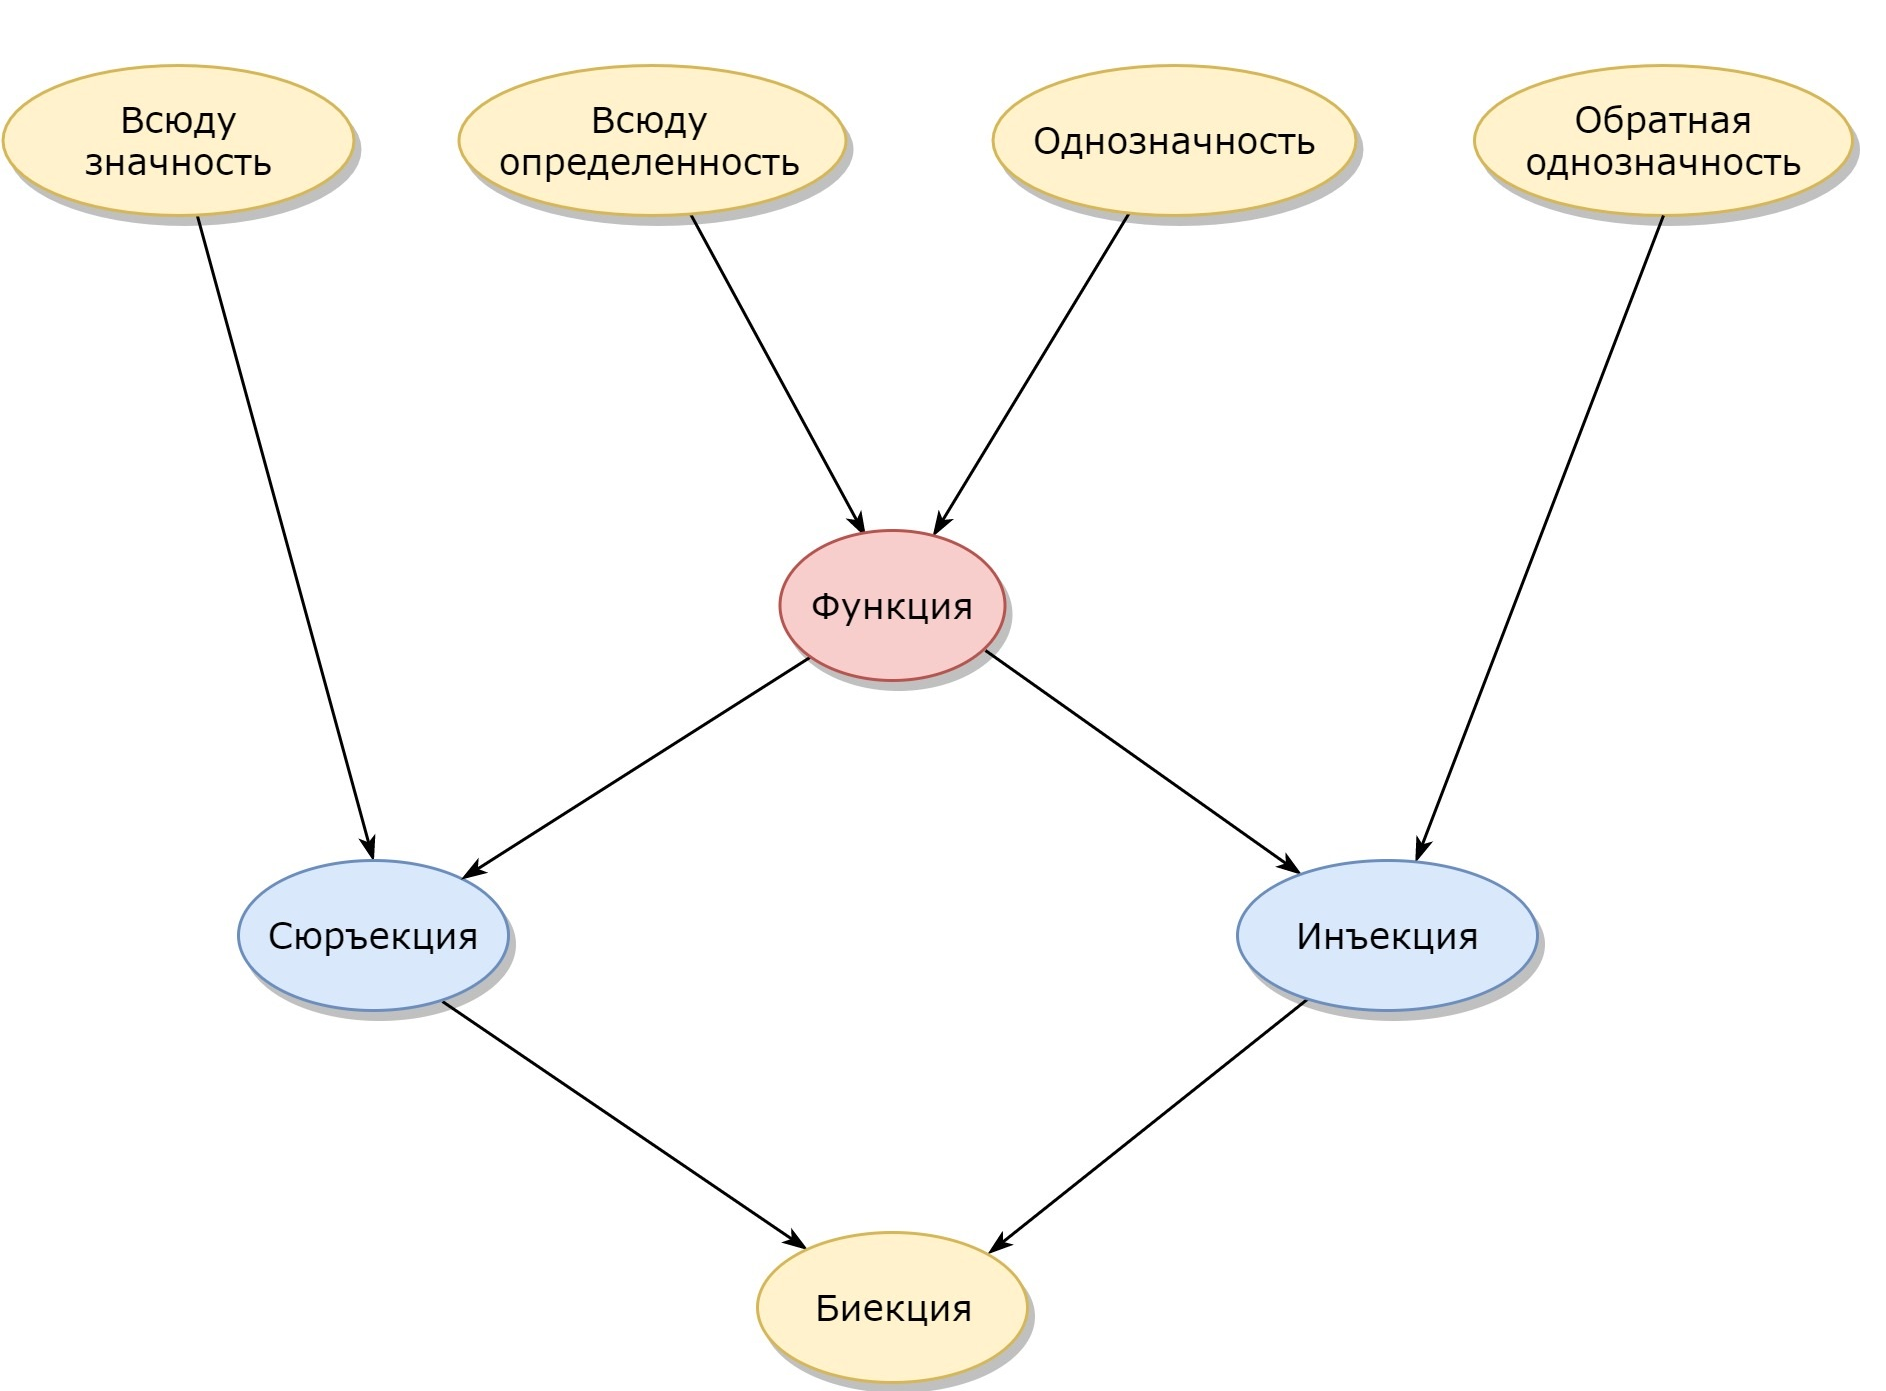
\includegraphics[scale=0.3]{function.png}
\end{center}

Обычно функция из $X$ в $Y$ обозначается $F:X\to Y$, а если $xFy$, то пишут $y=F(x)$. Для обозначения биекции часто используется символ $F:X\leftrightarrow Y$.
\item Обратным к $F$ отношение называется отношение $F^{-1}=\{(y,x)\mid xFy\}$. Если обратное отношение есть (частичная) функция, то она называется обратной функцией. Легко видеть, что $F(F^{-1}(y))=y$ и $F^{-1}(F(x))=x$, если только $F(x)$ и $F^{-1}(y)$ определены.
\item \textbf{Областью определения} (частичной) функции $F$ называется подмножество $X$, для элементов которого $F$ определена, \textbf{областью значений} (частичной) функции $F$ называется подмножество $Y$, для элементов которого $F$ определена.
\item Итак, функция --- это есть однозначное соответствие элементов одного множества элементам другого (или того же самого). Функции обычно задаются формулами, предписывающими некоторой алгоритм вычисления $y$ через $x$. Но иногда такие формул не указаны явно или же их указать вовсе невозможно, хотя существование функции доказывается. Ниже мы увидим пример такой теоремы (их еще называют теоремами существования).
\item Итак, как же сравнивать множества по числу элементов? Если мы возьмем конечное множество $A=\{a_1,\dots,a_n\}$, то мы сразу же подразумеваем наличие нумерации его элементов: номеру $k$ ставится в соответствие элемент $a_k$. И если все $a_k$ попарно различны, то в этом множестве столько же элементов, сколько чисел $1,\dots,n$, т.е. $n$ штук.
\item В этом рассуждении мы неявно указали на то, что существует взаимно однозначное соответствие между элементами множества $A$ и множеством-эталоном $\{1,\dots, n\}$.
\item Теперь, если задано некоторое множество $B=\{b_1,\dots,b_n\}$, у которого также все $b_k$ попарно различны, то мы внось имеем дело со взаимно однозначм соответствием между $B$ и множеством-эталоном $\{1,\dots, n\}$. Иначе говоря, мы имеем биекции 
$$
f:\{1,\dots, n\}\leftrightarrow A\mbox{ и }g:\{1,\dots, n\}\leftrightarrow B.
$$
\item Но тогда сложная функция $h(a)=g(f^{-1}(a))$ устанавливает взаимно однозначное соответствие между $A$ и $B$. Это можно проиллюстрировать на диаграмме:
\[ \begin{diagram}
\node{A} \arrow[2]{e,t}{g\circ f^{-1}}
\node[2]{B} \\
\node[2]{\{1,\dots,n\}} \arrow{ne,r}{g}
\arrow{nw,b}{f}
\end{diagram}\]

\item Таким образом, мы находим, что конечные множества $A$ и $B$ обладают одинаковой мощностью (количеством элементов), если между ними существует биекция.
\item Именно такой подход и выбирается при определении равномощности произвольных множеств!
\item Множества $X$ и $Y$ \textbf{равномощны} (будем это записывать так: $X\leftrightarrow Y$), если существует биекция $f:X\leftrightarrow Y$.
\item Заметим, что при этом мы не требуем наличия какого-то эталонного множества, хотя для конечных множеств, как мы уже видели, таковыми могут считаться множества $\{1,\dots,n\}$ или, как принято в теории множеств, множества $\{0,\dots,n-1\}$.
\item Отношение $\leftrightarrow$ рефлексивно (всякое множество само себе равномощно), симметрично (если $X\leftrightarrow Y$, то $Y\leftrightarrow X$) и транзитивно (если $X\leftrightarrow Y$ и $Y\leftrightarrow Z$, то $X\leftrightarrow Z$), т.е. является отношением эквивалентности. Это значит, что, вообще говоря, все множества можно разделить на непересекающиеся классы, так что внутри каждого класса будут находиться только равномощные множества. Такой класс и принято называть \textbf{мощностью множества}.
\item Другой подход к определению самого понятия мощности заключается в том, чтобы в каждом таком классе найти некоторого типичного представителя и его объявить мерой мощности всех множеств данного класса. В случае конечных множеств такими представителями как раз и являются отрезки натурального ряда $\{0,\dots,n-1\}$.
\item Множество, не содержащее элементов, т.е. пустое множество $\emptyset$, имеет мощность 0, оно биективно не сопоставляется ни с каким другим множеством, т.е. является уникальным представителем своего класса, и само себе является мерой мощности.
\item Еще одна разновидность множеств, имеющих эталон мощности --- \textbf{счетные множества}. К ним относятся все множества, равномощные $\N$.
\item Например, счетными являются такие множества:
$$
2\N,\Z,2\Z,\{p\in\N\mid p \mbox{--- простое}\},\Z[i],\Q,\A.
$$
Все множества, которые не конечны, и элементы которых можно перенумеровать (пересчитать) натуральными числами, являются счетными.
\item Нумерацию $2\N$ представить очень просто: каждому номеру $k$ поставим в соответствие элемент $2k$, тем самым мы перенумеруем все четные числа, а значит, множество четных чисел счетное. Здесь мы впервые сталкиваемся с тем, что бесконечное множество равномощно какой-то своей части (которая может казаться очень маленькой, ведь точно так же устанавливается биекция между $\N$ и $10^9\N$ и т.п.). Иногда такое свойство бесконечных множеств берется за их определение:\textit{ множество бесконечное, если оно равномощно некоторому своему собственному подмножеству}.
\item Биекцию $\N\leftrightarrow\Z$ установить также относительно просто: будем нумеровать целые числа по мере их удаления от нуля: $0, 1, -1, 2, -2, 3, -3$, и т.д. Ясно, что каждое целое число будет пронумеровано, и притом только один раз. Следовательно, $\Z$ --- счетное.
\item Для нумерации $\Z[i]$ нужно воспользоваться нумерацией змейкой: обходить все точки $\Z[i]$ по спирали, постепенно удаляясь от 0. Построим биекцию в обратную сторону, т.е. из $\Z[i]$ в $\N$, следующим способом:
$$
f(n+mi) = n+(n+m+1)(n+m)/2.
$$
Вспоминая теперь, что $\Z[i]=\Z\times\Z$ (если забыть об арифметике на этом множестве), то мы получаем замечательный факт, который называется \textbf{теоремой о квадрате}: $\Z\leftrightarrow\Z\times \Z$. То есть, счетное множество равномощно своего квадрату. Конечным множествам такое и не снилось!
\item Можно развить это достижение и дальше. Имея нумерацию $\Z\times\Z$ и $\Z$, мы можем пронумеровать $\Z\times\Z\times\Z$, т.е. куб множества $\Z$, и так далее. Любая конечная степень $\Z$ равномощна $\Z$.
\item Рациональные числа --- это пары целых чисел, но не всех, а только взаимно простых. Это значит, что они тоже получают номера в процессе нумерования $\Z\times\Z$, только с пропусками. Если затем эти номера перенумеровать заново, уже без пропусков, то мы получим взаимно однозначное соответствие $\Q$ и $\N$. То есть множество $\Q$ также счетно.
\item Для нумерации $\A$ воспользуемся следующим приемом. Вспомним, что $\A$ --- это все корни всех многочленов с целыми коэффициентами. Возьмем тогда некоторое целое положительное число $L$ и соберем в множество $\A_L$ те и только те алгебраические числа, которые определяются многочленами вида $P(x)=k_0+k_1x+\dots+k_nx^n$ ($k_n\ne 0$), удовлетворяющими условию
$$
|k_0|+|k_1|+\dots+|k_n|+n=L.
$$
Ясно, что таких многочленов существует лишь конечный набор, т.к. выбор коэффициентов $k_s$ и степени $n$ ограничен числом $L$. Но и корней у многочлена --- тоже конечное количество, не превышающее его степень (см. выше теорему о корнях над полем). Таким образом, множество $\A_L$ конечно.

С другой стороны, множество $\A$ есть объединение всех множеств $\A_L$ при $L=1,2,\dots$ Поэтому, нумеруя последовательно, сначала числа из $\A_1$, затем числа из $\A_2$, и т.д. мы пронумеруем все множество $\A$, а значит, это множество счетное!

\item Что же получается в итоге? Множество алгебраических чисел, которыми мы старались заткнуть все дыры между рациональными числами, и которое состоит из бесконечного числа бесконечных слоев, равномощно множеству $\Q$! С точки зрения мощности множества мы так ничего и не добавили к рациональным числам, хотя и позатыкали много дыр.
\item Возникает вопрос: \textit{а бывают ли вообще какие-то другие мощности, кроме счетной?} Ответ на этот вопрос дает
\begin{thrm}[Кантора]
Никакое множество не равномощно множеству всех своих подмножеств.
\end{thrm}
\pf
Пусть имеется множество $X$. Можем сразу считать, что оно непустое, т.к. для пустого множества теорема, очевидно, верна (в пустом множестве 0 элементов, а в множестве $\{\emptyset\}$ --- один элемент). Через $\Pcal(X)$ обозначим множество всех подмножеств множества $X$.

Предположим, что существует биекция $f:X\leftrightarrow\Pcal(X)$. Ясно, что поскольку для всякого $x\in X$ значение $f(x)$ есть какое-то подмножество $X$, то возможны две ситуации: либо $x\in f(x)$, либо $x\notin f(x)$. Соберем тогда в множество $Y$ все такие элементы $x$, которые удовлетворяют второму соотношению:
$$
Y=\{x\in X\mid x\notin f(x)\}.
$$
Понятно, что $Y\subseteq X$, а значит, $Y\in\Pcal(X)$, а значит, существует единственный элемент $y\in X$ такой, что $f(y)=Y$ (поскольку $f$ --- биекция по предположению).

Вопрос: $y\in Y$ или нет?

Если $y\in Y$, то по определению множества $Y$ получаем, что $y\notin f(y)$, но тогда $y\notin Y$. Противоречие.

Если $y\notin Y$, то по определению множества $Y$ получаем, что \textbf{неверно} $y\notin f(y)$, т.е. $y\in Y$. Противоречие.

Любой вариант приводит к противоречию, следовательно, предположение о существовании биекции $f:X\leftrightarrow\Pcal(X)$ неверно, т.е. множество $X$ и множество всех его подмножеств неравномощны.
\epf

Теорему Кантора можно дополнить тем, что множество всех подмножеств множества $X$ мощнее исходного множества $X$, т.к. $X$ в него инъективно вкладывается, т.е. равномощно некоторой части $\Pcal(X)$. Действительно, в $\Pcal(X)$ существует подмножество следующего вида:
$$
\{\{x\}\mid x\in X\},
$$
это --- множество всех синглетов (т.е. одноточечных подмножеств), образованных точками множества $X$. Таким образом, $\Pcal(X)$ получается более мощным множеством, чем $X$.

\item Приведем пример. Пусть $X=\{1,2,3\}$. Тогда
$$
\Pcal(X) = \{\emptyset,\{1\},\{2\},\{3\},\{1,2\},\{1,3\},\{2,3\},\{1,2,3\}\}.
$$
Подмножество синглетов здесь --- это множество $\{\{1\},\{2\},\{3\}\}$.

\item Для конечного множества $X$ мощности $n$ мощность множества его подмножеств $\Pcal(X)$ равна $2^n$. Это легко проверить, поскольку каждое подмножество $X$ задается состояниями его элементов: каждый из них может входить в данное подмножество или не входить. Поскольку у каждого элемента ровно 2 состояния, а всего элементов $n$, то общее количество состояний всех элементов равно $2\cdot 2\cdot\ldots\cdot 2$ ($n$ раз), т.е. $2^n$.
\item Отсюда берет начало второе обозначение для множества всех подмножеств множества $X$ --- $2^X$.
\item Но если с конечными множествми все укладывается в рамки обычно арифметики, то с множеством $2^\N$ возникают проблемы. Его мощность не только не выражается натуральным числом, но она также не равна и мощности $\N$, как мы только что доказали. Эта мощность называется \textbf{мощностью континуума} и обозначается $\cgot$.
\item Итак, мы теперь знаем, что бесконечные множества отличаются по мощности. Как же можно устанавливать их равномощность, если сложно или невозможно в явном виде указать биекцию между множествами? ответ на этот вопрос дает
\begin{thrm}[Кантора--Бернштейна]
Если существуют инъекции $f:A\to B$ и $g:B\to A$, то множества $A$ и $B$ равномощны.
\end{thrm}
\pf Рассмотрим функцию $H:2^A\to 2^B$, определяемую следующей формулой:
\[H(X)=A\setminus g[B\setminus fX]\mbox{ для всех }X\subseteq A.\]
\textit{Примечание}: здесь под записью $fX$ и $f[X]$ понимается \textbf{образ множества} $X$, т.е.
$$
f[X] = \{f(x)\mid x\in X\}.
$$

Предположим, что существует корень уравнения $H(X)=X$ --- некое множество $X_0$.
Посмотрим, какими свойствами оно обладает. Обозначим через $Y_0$ множество
$B\setminus fX_0$. Поскольку $H(X_0)=X_0$, то $gY_0=A\setminus X_0$. Таким
образом, сужения функций $f|_{X_0}$ и $g|_{Y_0}$ действуют на непересекающихся
подмножествах множеств $A$ и $B$ и <<покрывают>> эти множества
целиком.

Точнее, рассмотрим обратную к $g|_{Y_0}$ функцию, определенную на множестве
$A\setminus X_0$, обозначив ее $h$. Имеем: $h:A\setminus X_0\to Y_0$ ---
биекция, $f|_{X_0}:X_0\to B\setminus Y_0$ --- тоже биекция. Тогда объединение
этих функций $h\cup f|_{X_0}$ есть биекция между $A$ и $B$.

Итак, доказательство теоремы свелось к поиску корня уравнения $H(X)=X$. Назовем
множество $X$ {\itshape хорошим}, если $X\subseteq H(X)$ (почти как в теореме Кантора!), и через $Z$ обозначим
объединение всех хороших множеств.

Нетрудно проверить, что функция $H$ монотонна по вложению множеств, т.\,е.
если $X\subseteq Y$, то $H(X)\subseteq H(Y)$. Пусть $z\in Z$. Тогда существует
хорошее множество $X$ такое, что $z\in X$. Кроме того, имеем $H(X)\subseteq
H(Z)$ и $X\subseteq H(X)$. Отсюда заключаем, что $z\in H(Z)$, и это верно
для любого $z\in Z$. Таким образом, $Z$ --- хорошее множество.

Чтобы показать, что $Z$ и есть корень нашего уравнения, надо проверить обратное
вложение, т.\,е. что $H(Z)\subseteq Z$. Допустим, что это не так. Тогда
существует $x\in H(Z)\setminus Z$. Рассмотрим множество $Z'=Z\cup\{x\}$.
Это множество не может быть хорошим, т.\,к. иначе оно бы содержалось в $Z$.
Поэтому $Z'\not\subseteq H(Z')$. Ясно, что $H(Z)\subseteq H(Z')$, поэтому
$Z'\not\subseteq H(Z)$. С другой стороны, $Z\subseteq H(Z)$. Следовательно,
точка $x$ --- единственная точка множества $Z'$, не попадающая в $H(Z)$.
Получено противоречие с тем, что $x\in H(Z)$.

Итак, $H(Z)\subseteq Z$, откуда $H(Z)=Z$, т.\,е. $Z$ --- искомое множество.\epf

\item Теорема Кантора--Бернштейна дает достаточно простой инструмент сравнения мощностей. Достаточно показать, что первое множество равномощно какой-то части второго, а второе --- какой-то части первого, т.е. что они взаимно друг в друга вкладываются. Это будет означать, что между ними существует биекция, т.е. что они равномощны. При этом данная теорема не прдъявляет нам какого-то простого алогритма построения этой биекции, т.к. явно найти и описать все хорошие множества --- далеко не всегда разрешимая задача.
\item С помощью этой теоремы легко показать равномощность $\Q$ и натурального ряда. Действительно, $\Q$ легко вкладывается в часть множества $\Z\times \Z$ (пары взаимно простых составляют его часть). Но $\Z\times\Z$ мы умеем явно нумеровать целыми числами, т.е. умеем строить инъекцию из $\Z\times\Z$ в $\Z$, а значит, мы имеем вложение $\Q$ в $\Z$. Ну, а вложение в обратную сторону тривиально. Таким способом получается много результатов о равномощности.
\item Назовем множество \textbf{не более чем счетным}, если оно счетно или конечно (или пустое).
\begin{thrm}
Объединение не более чем счетного множества не более чем счетных множеств не более чем счетно.
\end{thrm}
\pf Мы можем считать, что нам дан счетный набор не более счетных множеств. При необходимости мы просто дополним этот набор до счетного пустыми множествами (ведь формулировка не требует, что они были разные). Раз их счетный набор, значит, они как-то уже пронумерованы. Пусть они обозначаются символами $A_n$. Тогда требуемое объединение равно
$$
A = \bigcup_{n=1}^\infty A_n,
$$
где все $A_n$ --- не более чем счетные множества.

Поскольку нам известно, что $A_n$ --- не более чем счетное, значит, существуют биекции $f_n$ между $A_n$ и либо $\N$, либо каким-то-конечным отрезком $\N$. В любом случае $f_n$ --- это инъекция из $A_n$ в $\N$.

Теперь построим инъекцию из $A$ в $\Z\times\Z$.

Пусть $a\in A$. Тогда существует $n$ такой, что $a\in A_n$. Может оказаться так, что $a$ лежит сразу во многих множествах $A_n$, в таком случае выберем нименьший из их номеров и обозначим его за $n_a$. Поскольку $a\in A_{n_a}$, мы можем применить к нему функцию $f_{n_a}$. Положим далее
$$
g(a) = (n_a,f_{n_a}(a)).
$$
Ясно, что $g$ --- инъекция, т.к. для разных точек $a$ и $a'$ либо отличаются номера $n_a$ и $n_{a'}$, и следовательно $g(a)\ne g(a')$ по свойствам упорядоченной пары, либо у них общий номер $n_a$, но тогда отличаются значения $f_{n_a}(a)$ и $f_{n_a}(a')$, поскольку $f_{n_a}$ является инъекцией, и, стало быть, $g(a)\ne g(a')$.

Итак, у нас есть инъекция $g:A\to\Z\times\Z$. К ней можно применить биекцию $f:\Z\times\Z\leftrightarrow\Z$, которую мы ранее выписывали в явном виде, а затем применить биекцию $h:\Z\leftrightarrow\N$, полагая $h(m)=2m$, если $m\ge 0$, и $h(m)=-2m-1$, если $m<0$. Тогда композиция $P=h(f(g(a)))$ будет инъекцией из $A$ в $\N$.

Область значений $P$ есть подмножество в $\N$. Она либо имеет максимум, и тогда это конечное множество, либо не имеет максимума, и тогда это бесконечное множество. В любом случае, область значений $P$ можно перенумеровать так, чтобы номера шли подряд от нуля без пропусков. И тогда с помощью $P^{-1}$ мы построим биекцию между $A$ и либо конечным отрезком натурального ряда, либо самим $\N$.\epf

\end{enumerate}


\section{Изоморфизмы}

\subsection*{Конспект}

\begin{enumerate}
\item Установление биекции между множествами позволяет нам судить об их количественном сходстве, но ничего не говорит о том, насколько похожи могут быть структуры, заданные на них. Поэтому на базе понятия биекции строятся более сильные критерии <<похожести>> двух множеств.
\item Центральным термином здесь является \textbf{<<изоморфизм>>}. Это --- биекция, сохраняющая операции (например, сложение или умножение) и/или отношения (например, линейный порядок или отношение эквивалентности) и/или функционалы (например, норма или длина), заданные на этих двух множествах.
\item Поясним. Пусть у нас задана группа $\Z_4$ со сложением по модулю 4, и группа корней 4 степени из 1 с операцией умножения (делители 1 в кольце гауссовых чисел). В обоих множествах 4 элемента, следовательно, существует биекция между ними. Причем, таких биекций ровно столько, сколько перестановок в группе $\Sb_4$, т.е. 24 штуки. Однако, если дополнительно потребовать, чтобы результат сложения двух элементов в первой группе переходил в результат умножения образов этих элементов во второй группе, то такая биекция окажется всего одна. Она-то и будет изоморфизмом этих групп.
\item Еще пример. Рассмотрим множества $\Z$ и $2\Z$ с обычныи операциями сложения и умножения, и обычным линейным порядком на них. Мы уже знаем, что эти множества равномощны. Но посмотрим повнимательнее на биекцию $f(n)=2n$, действующую из $\Z$ в $2\Z$. Оказывается, что:
$$
f(n+m)=f(n)+f(m),\quad n<m\Leftrightarrow f(n)<f(m),
$$
т.е. $f$ сохраняет сложение и порядок. А это значит, что $f$ является изморфизмом упорядоченных групп $(\Z,<)$ и $(2\Z,<)$.

Однако, $f$ не сохраняет умножение, поскольку $f(nm)=2nm\ne f(n)f(m)$. Следовательно, $f$ не является изоморфизмом колец $(\Z,+,\cdot)$ и $(2\Z,+,\cdot)$. Более того, эти два кольца вовсе неизоморфны. Дело в том, что изоморфизм должен сохранять единицу, т.е. если какое-то чисало $\e$ является единицей по умножению в первом кольце, то $f(\e)$ будет единицей во втором кольце. Просто потому, что $n\e=n$ соответствует $f(n)=f(n)f(\e)$. Но чему бы ни было равно $f(1)$ в кольце $2\Z$, оно не обладает свойствами единицы, а значит, эти кольца не изоморфны.
\item Бывает и еще хуже. Изоморфизм работает только по отношению порядка, но не работает по алгебраическим операциям. Для этого достаточно вспомнить два изученных нами поля: $\Q$ и $\A$.
\item Ясно, что эти поля не могут быть изоморфны по операциям, т.к. иначе в обоих полях одинаково бы разрешалось или не разрешалось уравнение $x^2=2$. Но мы знаем, что оноразрешается в $\A$ и не разрешается в $\Q$. Тем неменее, с порядковым изоморфизмом у них все в порядке.
\begin{thrm} Все счетные неограниченные сверху и снизу плотные линейно упорядоченные множества порядково изоморфны.\end{thrm}
Иначе гвооря, пусть у нас имеется два множества $A$ и $B$, которые счетны (т.\,е. все их элементы можно перенумеровать натуральными числами), на них заданы линейные порядки $<_A$ и $<_B$ такие, что в обоих множествах нет ни наибольшего, ни наименьшего элемента, и эти множества плотны в своем порядке, тогда существует изоморфизм $f:A\leftrightarrow B$, сохраняющий порядок, т.е. $f(x)<_Bf(y)\Leftrightarrow x<_Ay$.
\pf
Будем строить соответствие пошагово. Пусть мы сделали некоторое соответствие для подмножеств $A_n\subset A$ и $B_n\subset B$ из $n$ элементов. Возьмем любой элемент одного из множеств (для определенности $A$), который не вошел в $A_n$. Посмотрим, в каком отношении он находится со всеми элементами из $A_n$. Он оказался либо наибольшим элементом, либо наименьшим элементом, либо стоящим между некоторыми элементами $a_i$ и $a_{i+1}$. Найдем элемент в $B$, находящийся в таком же отношении со всеми элементами $B_n$. Мы можем это сделать, так как $B$ --- плотное множество без наибольшего и наименьшего элементов. Будем считать эти два элемента сопоставленными. Таким образом, мы научились получать из соответствия для $n$ элементов соответствие для $n+1$ элемента. Чтобы в пределе получить соответствие для всех элементов, воспользуемся счетностью множеств $A$ и $B$. Пронумеруем все элементы и на каждом четном шаге будем выбирать еще не взятый элемент из множества $A$ с наименьшим номером, а на нечетном --- из $B$.
\epf

Из этой теоремы следует, например, что множество $\Q$ с обычным линейным порядком и множество $\A$ всех алгебраических чисел с обычным линейным порядком порядково изоморфны! Больше того, рациональный интервал $(a;b)$ порядково изоморфен всему множеству  $\Q$.
\end{enumerate}



\section{Действительные числа}

\subsection*{Конспект}

\begin{enumerate}
\item Вспомним снова про множество $\B$, которое состоит из рациональных чисел вида $k/2^n$, где $k\in\Z$, $n\in\N$.
\item Это множество есть собственное подмножество $\Q$. Оно счетно и всюду плотно. Но главное --- оно очень удобно устроено.
При $n=0$ мы имеем целочиселнную решетку на числовой прямой, при $n=1$ мы получаем все целые и полуцелые числа, при $n=2$ --- все числа с шагом $1/4$. Обозначим
$$
\B_n=\{k/2^n\mid k\in\Z\}.
$$
Тем самым мы определяем некоторый слой в множестве $\B$ с фиксированным шагом, равным $1/2^n$.
\item Множества $\B_n$ хороши тем, что образуют возрастающую последовательность по вложению, которая стартует с $\Z$ и заканчивается $\B$:
$$
\Z=\B_0\subset\B_1\subset\B_2\subset\dots\subset\B
$$
В таком случае принято называть множество $\B$ \textbf{пределом возрастающей цепи множеств}.
\item Поскольку расстояние между соседними точками $\B_n$ очень быстро сокращается с ростом $n$, то любая точка на прямой может быть сколь угодно точно приближена точками множества $\B$.
\item Процесс последовательного приближения произвольной точки $A$ на числовой прямой можно осуществить следующим образом.
\begin{enumerate}[{\bf Step1}]
\item Находим целое число $k$ такое, что точка $A$ лежит в полуинтервале $[k;k+1)$, т.е. либо между соседними целыми числами, либо совпадает с целым числом. Очевидно, что такое $k$ определяется однозначно и всегда существует. Обозначим отрезок $[k;k+1]$ за $\De_0$. Ясно, что его границы $k$ и $k+1$ есть элементы множества $\B_0$.
\item Пусть далее $n$ --- это номер текущего интервала (начиная с нуля).
\item Находясь в отрезке $\De_n$, делим его на 2 части посередине так, чтобы получилось два одинаковых полуинтервала: если $\De_n=[a;b]$, то новые полуинтервалы будут $[a;(a+b)/2)$ и $[(a+b)/2;b)$. Точка $A$ лежит в одном из этих полуинтервалов: либо в левом, либо в правом, третьего не дано.

Заметим, что и границы $\De_n$, и его середина --- это точки множества $\B$, причем границы $\De_n$ находятся в множестве $\B_n$, а его середина --- в множестве $\B_{n+1}$. Таким образом, это подразбиение является переходом к следующему уровню разбиения в множестве $\B$.
\item Тогда через $\De_{n+1}$ обозначим отрезок $[a;(a+b)/2]$, если $A\in[a;(a+b)/2)$, и отрезок $[(a+b)/2;b]$, если $A\in[(a+b)/2;b)$. После чего перейдем на предыдущий шаг, увеличивая номер $n$ на 1.
\end{enumerate}

В результате мы получим последовательность вложенных отрезков
$$
[k;k+1]=\De_0\supset\De_1\supset\De_2\supset\dots
$$
Эта последовательность монотонно убывает, причем на каждом шаге отрезок становится вдвое короче, а концы отрезков прыгают по точкам множества $\B$, постепенно переходя ко все более мелкой сетке --- от $\B_n$ к $\B_{n+1}$.

\item Где же в итоге окажется точка $A$?
\item Поскольку $A\in\De_n$ для всех $n$, то она также лежит в пересечении всех этих отрезков:
$$
A\in\bigcup_n\De_n.
$$
Такое пересечение называется пределом убывающей цепи множеств.
\item Может ли в этом пересечении лежать еще какая-то точка? Ответ: нет. Если мы возьмем любую другую точку $B\ne A$, то, очевидно, что между ними есть какое-то расстояние $\ep>0$. Возьмем тогда такое $n$, что $\ep>1/2^n$, и посмотрим на отрезок $\De_n$. Еого длина равна $1/2^n$ и он содержит точку $A$. Но тогда он не содержит точку $B$, а значит, и пересечение всех отрезков $\De_n$ не содержит точку $B$.
\item Итак, точка $A$ --- единственный представитель пересечения отрезков $\De_n$:
$$
\bigcap_n\De_n = \{A\}.
$$
\item По сути, мы уже сформулировали главный принцип непрерывности (полноты) числовой прямой --- принцип вложенных отрезков. Однако, здесь нужно проявить осмотрительность. Дело в том, что мы не доказали существование точки $A$, а сразу же выбрали ее из существующих точек прямой. Но в настоящий момент нам известны только рациональные числа и алгебраические, поэтому разумно ожидать, что точка $A$ есть одно из таких чисел. Но рассмотренный принцип <<ловли>> произвольной точки на прямой с помощью стягивающейся сетки двоично-рациональных чисел сам по себе является мощным инструментом для определения новых чисел и, что самое главное, для ликвидации всех возможных дыр на числовой оси, состоящей из алгебраических чисел.
\item На самом деле, вовсе не очевидно, что если мы выберем произвольную последовательность вложенных отрезков, длина которых стремится к нулю с ростом номера, то в пределе получим множество, состоящее из одной точки. Быть может, никакой точки там вовсе не окажется. Поэтому приходится вводить принцип непрерывности при помощи \textbf{аксиомы непрерывности} (она же --- аксиома полноты).
\item У этой аксиомы существует много равносильных формулировок, и мы начнем с той, к которой нас подготовил сюжет по поимке точки $A$ в сеть множества $\B$.
\item[{\bf A1}] \textbf{Принцип вложенных отрезков}. Пусть дана последовательность вложенных отрезков на прямой:
$$
[a_0;b_0]\supseteq[a_1;b_1]\supseteq[a_2;b_2]\supseteq\dots[a_n;b_n]\supseteq\dots,
$$
где $a_n<b_n$ для всех $n$. Тогда множество точек, принадлежащих всем отрезкам одновременно, не пусто.
\item В терминах, которые мы упоминали выше, принцип A1 можно переформулировать так: любая убывающая по вложению бесконечная цепь отрезков имеет непустой предел.
\item Отметим, что в формулировке мы не требовали, чтобы концы отрезков были двоично-рациональными числами, а также не требовали, чтобы их длина стремилась к нулю. Очевидно, что случай с двоично-рациональными отрезками является частным случаем последовательности вложенных отрезков, а значит, в силу принципа \textbf{A1} имеет непустой предел.

На самом деле, если сформулировать принцип вложенных отрезков, используя только двоично-рациональные концы отрезков и деление отрезка пополам на каждом шаге, мы получим эквивалентную формулировку принципа вложенных отрезков. Но доказательство этого факта мы оставим за рамками курса.
\item Принцип вложенных отрезков уже позволяет нам доказать, что на числовой прямой существуют не только алгебраические числа, более того, что точек на прямой существует несчетное множество.

Предположим, что это не так, и пусть на прямой есть только счетный набор точек. В соответствии с определением счетности мы можем перенумеровать все эти точки натуальными числами $x_0,x_1,x_2,\dots$

Построим цепь вложенных отрезков следующим способом. Выберем любой отрезок $\De_0$ (можно считать, что он имеет концы в множестве $\B$, но это не обязательно) так, чтобы $x_0\notin\De_0$. Точка $x_1$ может лежать или не лежать в отрезке $\De_0$, но в любом случае мы можем выбрать отрезок $\De_1$ так, чтобы выполнялись условия: $\De_1\subseteq\De_0$ и $x_1\notin\De_1$. Заметим, что при этом также $x_0\notin\De_1$. Далее, точка $x_2$ может лежать или не лежать в отрезке $\De_1$, но мы всегда можем выбрать отрезок $\De_2\subseteq\De_1$ так, чтобы $x_2\notin\De_2$. Продолжаем эту процедуру до бесконечности, поддерживая следующую ситуацию:
$$
\De_{n+1}\subseteq\De_n,\quad x_0,\dots,x_{n+1}\notin\De_{n+1}.
$$

Но тогда в пересечении $\cap\De_n$ нет ни одной точки $x_n$, т.е. нет вообще ни одной точки числовой прямой. Но в силу принципа \textbf{A1} там должна быть хотя бы одна точка. Противоречие.

Таким образом, принцип вложенных отрезков гарантирует нам несчетность множества чисел на прямой. Насколько велико это множество, мы сможем оценить чуть позже.
\item Следующее, что можно отметить, опираясь на наш пример с поимкой точки $A$ в сеть множества $\B$, это что последовательность левых границ вложенных отрезков не убывает. На каждом шаге левая граница $\De_n$ либо остается такой же, как у предыдущего отрезка, либо перескакивает в его середину. Но при этом все левые границы отрезков $\De_n$ остаются ограниченными сверху правой границей начального отрезка $\De_0$. То же самое мы видим и в ситуации с произвольной последовательностью вложенных отрезков, которую мы описываоли при формулировке принципа \textbf{A1}.
\item Аналогичное наблюдение можно вывести и для правых концов вложенных отрезков. Мы имеем некую бесконечную монотонную последовательность точек, и притом ограниченную, т.е. находящуюся в некотором заранее известном отрезке.
\item Введем определения. Последовательность $\{x_n\}_{n=0}^\infty$ называется \textbf{убывающей} (или \textbf{возрастающей}), если для всех $n$ выполняется неравенство $x_n\ge x_{n+1}$ ($x_n\le x_{n+1}$). Убывающие и возрастающие последователности называются \textbf{монтонными}. Последовательность \textbf{строго} монотонна (строго убывающая или строго возрастающая), если указанное неравенство всегда строгое.

Множество $X$ на прямой называется \textbf{ограниченным сверху}, если существует точка $a$ такая, что $X\le a$.\footnote{Мы ранее уже вводили сравнение множеств и множеств с точкой. $X\le Y$, если для всех $x\in X,y\in Y$ имеем $x\le y$. $X\le a$, если $X\le\{a\}$. } Если ситуация противоположная, т.е. $X\ge a$, то множество $X$ называется \textbf{ограниченым снизу}. Если множество ограничено сверху и снизу, то но называется \textbf{ограниченным}.

Последовательность ограничена (сверху и/или снизу), если ограничено ее множество значений (сверху и/или снизу). отметим, что последовательность мы рассматриваем не просто как множество точек на прямой, а как функцию из $\N$ в множество точек прямой или любое другое множество. Это позволяет рассматривать, например, стационарные последовательности, когда $x_n=\const$, или циклические последовательности, когда $x_n$ принимает конечный набор значений, последовательно повторяя их. Например, $x_n=n\pmod m$ повторяет значения $0,1,\dots,m-1$.

\item Имея любую монотонную ограниченную последовательность, мы легко можем выстроить цепь вложенных отрезков. Если эта последовательность неубывающая, то в качестве левых границ отрезков берем ее элементы, а правую границу зафиксируем в какой-то одной точке, которая точно больше всех членов последователности (ее существование следует из ограниченности последовательности).
\item Можем усилить эффект, если в качестве правых границ вложенных отрезков на $n$-ом шаге выбирать наименьшее из чисел множества $\B_n$, превосходящих все оставшиеся члены последовательности.
$$
a_n=x_n,\quad b_n=\min\{q\in\B_n\mid \forall j\ge n\;x_j\le q\}
$$
В этом случае последовательность $b_n$ будет убывающей, причем она будет очень быстро сближаться с <<хвостом>> последовательности $\{x_n\}$, т.к. шаг между соседними числами в множетсве $\B_n$ равен $1/2^n$. И тогда длина отрезка $[a_n;b_n]$ с каждым шагом будет становиться все меньше, так что в предельном множестве, существование которого нам гарантирует принцип \textbf{A1}, не сможет находиться две и более точек. А та единственная, которая останется внутри пересечения всех $[a_n;b_n]$, будет пределом последовательности $\{x_n\}$, т.е. такой точкой, к которой данная последовательность приближается вплотную, не оставляя никакого зазора.
\item Введем одно из основных понятий математического анализа. Число $a$ называется \textbf{пределом последовательности} $\{x_n\}$ и обозначается
$$
a = \lim_{n\to\infty}x_n,
$$
если для любого $\ep>0$ существует такой номер $N$, что для всех $n>N$ имеет место неравенство $|x_n-a|<\ep$. Если последовательность $\{x_n\}$ имеет предел, то она называется \textbf{сходящейся} (к данному пределу), в противном случае --- \textbf{расходящейся}.

Назовем интервал $(a-\ep;a+\ep)$ $\ep$--окрестностью точки $a$. Ясно, что утверждение $|x_n-a|<\ep$ означает, что $x_n$ лежит в $\ep$--окретности точки $a$. Кроме того, очень часто говорят <<почти все члены последовательности>>, когда имеют ввиду некоторый ее хвост, т.е. ту же последовательность, но за исключением, быть может, какого-то ее конечного начального отрезка. Поэтому тот факт, что $a$ является пределом последовательности $\{x_n\}$, можно записать следующими словами: \textit{в любой сколь угодно малой окрестности точки $a$ лежат почти все члены последовательности} $\{x_n\}$.

Стоит отметить, что символика пределов в обязательном порядке предписывает указывать, при каком именно изменении параметра совершается предельный переход. В нашем случае параметром последовательности является индекс (или номер) ее членов, т.е. число $n$. И если еще раз внимательно прочитать определение предела, а также смысл фразы <<почти все члены последовательности>>, то мы увидим, что требование малого отклонения от предела выполняется при больших $n$, т.е. при $n>N$ при некотром номере $N$, который, вообще говоря, зависит от выбранного $\ep$. И весь смысл данного предела в том, что при забегании индекса $n$ в сторону бесконечности величина $x_n$ становится близкой к $a$.

Кроме того, параметров может быть несколько, и поэтому всегда следует указывать, относительно какого из них осуществляется предельный переход.

Приведем пример. Пусть $x_{n,m}=m/(1+(n-m)^2)$. Найдем ее предел при $n\to\infty$. Мы можем построить экспериментальный график и убедиться в том, что предел равен нулю.
\begin{center}
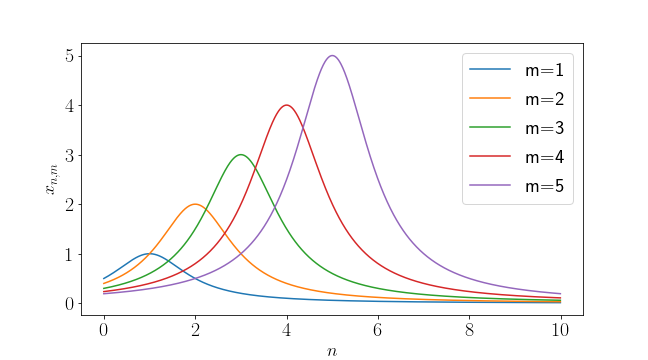
\includegraphics[scale=0.5]{limits.png}

График $\displaystyle x_{n,m}=\frac{m}{(1+(n-m)^2)}$.
\end{center}

Докажем, что так оно и есть на самом деле. Выберем произвольный достаточно малый $\ep>0$. Поскольку $x_{n,m}>0$, нам достаточно установить, при каких $n$ выполняется неравенство $x_{n,m}<\ep$, что и будет означаьт близость к нулю. Решая это неравенство, находим, что
$$
n>m+\sqrt{\frac{m}{\ep}-1},
$$
откуда видно, что начиная с некоторого $N$ (например, можно округлить вверх корень и добавить $m$) для всех последующих $n$ требуемое неравенство выполняется. Стало быть, по определениею получаем, что
$$
\lim_{n\to\infty}\frac{m}{(1+(n-m)^2)}=0.
$$

Однако, даже по графику видно, что если мы будем менять параметр $m$ вместо $n$, то мы увидим неограниченный рост величины $x_{n,m}$, так что ее предел при $m\to\infty$ и любом фиксированном $n$ будет равен $+\infty$.

Но и это еще не все. Можно так подобрать зависимость параметров $n$ и $m$ (например, положить $m=t^2$ и $n=t^2+t$, тогда получим $x_{n,m}=t^2/(1+t^2)\to 1$ при $t\to\infty$), что $x_{n,m}$ будет сходиться к любому наперед заданному положительному числу.

Поэтому всегда очень важно указывать, при каком изменении какого параметра ищется предел.

\item Из рассуждений, проведенных выше относительно монотонной ограниченной последовательности, ясно, что она должна иметь предел в силу принципа \textbf{A1}. На самом деле, верно как это, так и обратное: если монотонные ограниченные последовательности имеют предел, то выполняется принцип вложенных отрезков. Это совсем легко установить, поскольку границы вложенных отрезков образуют две монотнные ограниченные последовательности, а значит, имеют пределы. Причем как эти пределы, так и точки, лежащие между ними, будут принадлежать пределу цепи вложенных отрезков.
\item[\bf A2] \textit{Всякая монотонная ограниченная последовательность имеет предел}.\footnote{Если быть точным, то еще требуется архимедовость системы чисел, в котрой этот принцип постулируется, но для числовой прямой, в которой множество $\Z$ не ораничено ни сверху, ни снизу, это выполняется автоматически.}
\item Принцип \textbf{A2} равносилен принципу \textbf{A1}.
\item Следующее, что мы можем заметить из сюжета с поимкой точки $A$ сетью точек множества $\B$, это то, что границы отрезков не просто стремятся к точке $A$, но и как бы стремятся друг к другу, т.е. расстояния между всеми членами последовательности, начиная с некоторого номера, становятся сколь угодно малыми. Поэтому, даже ничего не зная о существовании предела, мы можем сделать некоторые выводы о последовательности.
\item Последовательность $\{x_n\}$ называется \textbf{фундаментальной}, если для любого $\ep>0$ существует такой номер $N$, что для всех номеров $n,m>N$ выполняется $|x_n-x_m|<\ep$. Иными словами, \textit{почти все члены фундаментальной последовательности находятся сколь угодно близко друг к другу}.
\item[\bf A3] \textit{Всякая фундаментальная последовательность имеет предел}.
\item Принцип \textbf{A3} равносилен двум предыдущим принципам.
\item Мы уже говорили о том, что множество может быть ограничено сверху или снизу. Пусть $X$ ограничено сверху числом $a$. Тогда число $a$ называется его \textbf{верхней гранью}. Ясно, что если $a$ --- верхняя грань $X$, то верхними гранями будут также $a+1, a+10000, a+0.0001$  и т.д. Все числа, большие $a$, будут верхними гранями $X$.
\item Вспомним уравнение $x^2=2$. Пусть $X=\{x\mid x^2<2\land x>0\}$. Это есть интервал $(0;\sqrt 2)$. Мы помним, что в $\Q$ нет числа $\sqrt 2$, поэтому в рамках множества $\Q$ верхними гранями $X$ будут положительные рациональные числа $r$ такие, что $r^2>2$. И среди этих чисел нет наименьшего, т.к. он недостижимо в $\Q$. Однако, стоит нам выйти в поле алгебраических чисел, как мы уже можем использрвать $\sqrt 2$, и он будет не просто верхней гранью $X$, а наименьшей их всех верхних граней.
\item Наименьшая из верхних граней $X$ называется \textbf{супремумом} $X$ или \textbf{точной верхней гранью} $X$.
\item Предлагаем читателю самостоятельно определиьт понятие точной нихней грани.
\item К точной верхней грани $X$ мы можем подбираться, находясь внутри $X$, выбирая каждый раз все новое число из $X$, находящееся как можно ближе к его верхней грани. Например, у цепи вложенных отрезков есть множество левых границ, образующее возрастающую последовательность. При этом все правые границы отрезков будут верхними гранями для этой последовательности. И если в пределе получится множество, состоящее из одной точки (как в сюже с ловлей точки $A$ точками множества $\B$), то эта точка и будет точной верхней гранью для последовательности левых границ вложенных отрезков.
\item Мы снова видим некоторую связь между существованием супремума и аксиомой непрерывности в ее трех предыдущих формулировках. На самом деле, эта связь абсолютная.
\item[\bf A4] Всякое ограниченное сверху множество имеет точную верхнюю грань.
\item[\bf A4'] Всякое ограниченное снизу множество имеет точную нижнюю грань.
\item Эти два принципа непрерывности эквивалентны друг другу и трем предыдущим принципам.
\item Наконец, заметим, что существует некоторая двойственность между верхними и нижними гранями и точныи гранями. Так, если взять некоторое множество $X$, ограниченное сверху, то оно само будет множеством нижних граней (не обязательно всех) для множества $Y$ своих верхних граней. При этом окажется, что $\sup X=\inf Y$. Аналогичная ситуация и с ограниченным снизу множеством. Возникает желание разбить всю числовую прямую на два луча --- левый и правый, --- так, чтобы левый был множеством нижних граней для верхнего и наоборот. Такое разбиение называется сечением.
\item В соответствии с определением, данным в разделе \ref{Ordering},
пара $(X,Y)$ непустых подмножеств, таких, что их объединение $X\cup Y=\Q$, $X\cap Y=\emptyset$ и $X<Y$, называется \textbf{сечением}.\footnote{Иногда определяется только нижний класс, и он называется сечением. Оба определения эквивалентны.}
\item Ранее мы уже видели такое разбиение. Оно представляло собой два интервала рациональных чисел: $(-\infty;\sqrt 2)$ и $(\sqrt 2;+\infty)$. Действительно, их объединение равно $\Q$, пересечение пусто, и левый интервал меньше правого.
\item В случае $\Q$ сечение может состоять их двух интервалов, т.е. таких множеств, что верхнее не имеет минимума, а нижнее не имеет максимума, и при этом между ними ничего нет. И это говорит нам о том, что в $\Q$ имеются дырки. В случае $\A$ дырки найти сложнее, но, например, разбиение на интервалы $(-\infty;\pi)$ и $(\pi;+\infty)$ доставляет такой пример, поскольку число $\pi$ не является алгебраическим.\footnote{Этот факт был доказан только в XX веке!}
\item Так вот, еще один подход к определению непрерывности числовой прямой заключаетсы в том, чтобы исключить такие дырки.
\item[\bf A5] Если $(X,Y)$ --- сечение числовой прямой, то существует точка $z$ такая, что $X\le z\le Y$.
\item При этом точка $z$ обязана попасть либо в верхний, либо в нижний класс разбиения, т.е. всякое сечение числовой прямой должно быть дедекиндовым (в соответствии с данным нами определением в разделе \ref{Ordering}). Иначе говоря, принцип \textbf{A5} утверждает, что линейный порядок на числовой прямой должен быть непрерывным.
\begin{figure}
\begin{center}
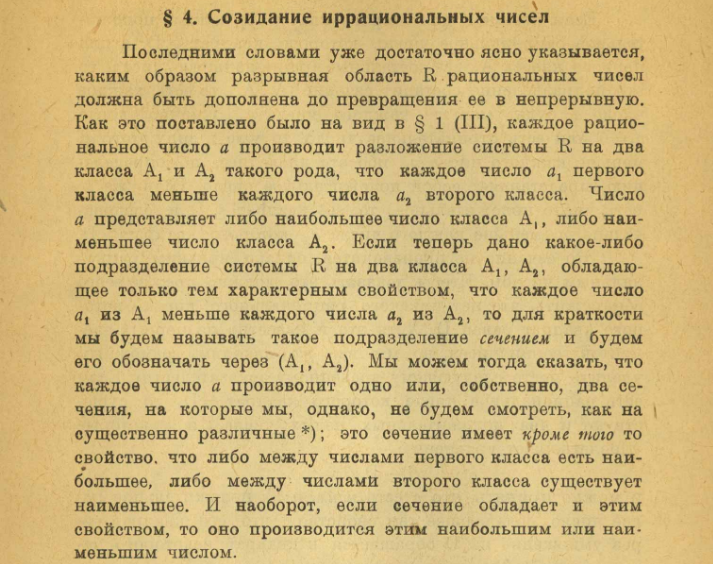
\includegraphics[scale=0.6]{dedekind.png}
\caption{Цитата из работы О.Дедекинда <<Непрерывность и иррациональные числа>> в пер. Шатуновского, 1923.}
\end{center}
\end{figure}
\item Формулировка аксиомы непрерывности в виде принципа \textbf{A5} эквивалентна всем предыдущим формулировкам \textbf{A1--A4}.
\item Наконец, самое главное определение данной главы. Числовая прямая, удовлетворяющая аксиоме непрерывности, называется \textbf{вещественной (действительной) прямой} и обозначается $\R$.

\item Если мы соберем вместе все накопленные свойства $\R$, то мы увидим, что $\R$ --- это \textit{непрерывное линейно упорядоченное поле}. Известно, что такое поле единственное с точностью до изоморфизма, сохраняющего  операции поля и линейный порядок.

\end{enumerate}


\subsection*{Задачи}
\begin{enumerate}
\item Доказать, что между любыми двумя рациональными числами $r\ne q$ лежит какое-то двоично-рациональное.
\item 
\item 
\item 
\item 
\item 
\end{enumerate}


\section{Модели действительных чисел}

\subsection*{Конспект}
\begin{enumerate}
\item В предыдущем разделе было сформулировано пять вариантов аксиомы непрерывности, которая необходима для того, чтобы узаконить действительные числа как непрерывную числовую структуру. Аксиома непрерывности не оставляет дыр на числовой прямой, поскольку вводит в обращение все числа, к которым можно обратиться с помощью счетной последователньости рациональных чисел.
\item Тем не менее, одной лишь аксиомы недостаточно, чтобы действительные числа имели право на существование. Необходимо убедиться в том, что их можно непротиворечиво сконструировать. Поэтому здесь мы рассмотрим несколько подходов к построению действительных чисел.

\subsection*{Дедекиндовы сечения}

\item Первый подход связан непосредственно с тем, чем мы закончили предыдущий раздел --- с дедекиндовыми сечениями. А именно, рассмотрим все сечения множества рациональных чисел, причем только такие, у которых нижний класс не содержит наибольшего элемента (т.е. если есть между классами граница, то она отнесена к верхнему классу). И соберем в множество $R$ нижние классы всех таких сечений. Таким образом, $R$ состоит из подмножеств $X\subset\Q$ таких, что
$$
X\ne\emptyset,\quad X\ne\Q,\quad\forall r,q\in\Q\;(q\in X)\land(r<q)\to(r\in X),\quad\not\exists\max X.
$$
Таким образом, $R$ --- это множество лучей из рациональных чисел, направленных в $-\infty$.
\item На множестве $R$ введем операцию сложения: пусть $\al,\be\in R$, тогда положим
$$
\al+\be = \{x+y\mid x\in \al,y\in \be\},
$$
т.е. просто сложим их по Минковскому.
\item Можно проверить, что $R$ с такой операцией сложения является абелевой группой, т.е. сложение ассоциативно, коммутативно, имеется нейтральный элемент $0=\{x\in\Q\mid x<0_\Q\}$, где $0_\Q$ --- ноль в системе рациональных чисел, и для каждого $\al$ имеется противоположный элемент $-\al=\{x\in\Q\mid (-x>\al)\land (-x\ne\min\Q\setminus\al)\}$.

Здесь появляется первая тонкость определения. По сути, в качестве $\al$ мы берем соответствующий ему верхний класс сечения и умножаем на -1 (в поле рациональных чисел). Однако верхний класс может иметь минимум, а элемент $R$ не должен иметь максимума, поэтому мы подстраховываемся и выбрасываем из верхнего класса $\Q\setminus\al$ его минимум (если такой существует).

\item Достаточно легко определяется и порядок на $R$. Скажем, что $\al<\be$, если $\al\subset\be$ (как собственое подмножество).
\item Отсюда же следует согласованность сложения и порядка, поскольку сдвиг вверх или вниз интервалов $\al<\be$ не меняет их вложенности.
\item Сложнее дело обстоит с умножением. Если мы попытаемся умножить $\al\cdot\be$ по Минковскому, то произведение будет содержать сколь угодно большие числа (при перемножении двух чисел, сильно меньших 0 в поле $\Q$). Поэтому сначала определяется произведение положительных чисел: пусть $\al>0$ и $\be>0$, тогда
$$
\al\cdot\be = \{xy\mid (x\in\al)\land(x\ge 0)\land(y\in\be)\land(y\ge 0)\}\cup\Q^-,
$$
где $\Q^-$ --- все отрицательные рациональные числа.

Далее, просто полагаем, что
$$
\al\cdot\be = 
\begin{cases}
0           ,&\mbox{ если }(\al=0)\lor(\be=0) \\
(-\al)\cdot\be,&\mbox{ если }(\al<0)\land(\be>0) \\
\al\cdot(-\be),&\mbox{ если }(\al>0)\land(\be<0) \\
(-\al)\cdot(-\be),&\mbox{ если }(\al<0)\land(\be<0)
\end{cases}
$$
\item Можно проверить, что такая операция умножения на $R$ ассоциативна, коммутативна, имеет единицу $1=\{x\in\Q\mid x<1_\Q\}$, где $1_\Q$ --- единица в системе рациональных чисел, и для каждого положительного $\al\in R$ имеется обратный по умножению
$$
1/\al = \{x\in\Q\mid \exists y>\al\;(x<1/y)\},
$$
а обратный к отрицательному числу определяется сменой знака: $1/\al=-(1/(-\al))$, если $\al<0$.
\item Кроме того, можно доказать, что операции сложения и умножения удовлетворяют дистрибутивному закону, а также что умножение согласовано с порядком.
\item Таким образом, $R$ с указанными операциями и порядком есть упорядоченное поле. Остается показать его непрерывность.
\item Для этого воспользуемся формулировкой аксиомы непрерывности в виде \textbf{A4}. Пусть $X\subset R$ непусто и ограничено сверху. Положим $\al=\cup X$. Т.е. мы включаем в множество $\al$ все рациональные числа входящие во все элементы множества $X$. Легко видеть, что $X\le\al$ (в смысле сравнения множества и числа в лнейном порядке на $R$). В то же время любая верхняя грань $X$ окажется не меньше $\al$, иначе она бы отсекла какое-то рациональное число одного из элементов $X$. Таким образом,
$$
\sup X=\cup X.
$$
\item Итак, множество $R$, построенное из подмножеств $\Q$ специального вида, с заданными на нем операциями и порядком, является непрерывным упорядоченным полем, т.е. полем действительных чисел $\R$.

\subsection*{Двочиные дроби}

\item Следующий подход к моделированию $\R$ прямо связан с нашим множеством $\B$. Вспомним сюжет о поимке точки $A$ в сеть точек множества $\B$, т.е. рациональных точек со знаменателями вида $2^n$. Мы выстраивали убывающую цепь отрезков, концы которых находятся в множестве $\B_n$, т.е. имеют вид $[k/2^n;(k+1)/2^n]$. Длина этих отрезков быстро стремится к нулю, а по аксиоме непрерывности в форме \textbf{A1} существует непустой предел этой цепи отрезков, который состоит из единственной точки $A$.
\item Почему бы тогда не обращаться к точке $A$ с помощью этой последовательности? Точнее, мы определим некоторый условный код, который позволит нам однозначно поймать точку $A$ и никакую другую.
\item Вспомним алгоритм построения этих отрезков. Сначала мы выбираем целочисленный полуинтервал $[k;k+1)$, в котором лежит $A$. Ок --- запишем число $k$ как стартовое число кода.
\item Затем мы делим этот интервал ровно пополам: $[k;k+1)=[k+1/2)\cup[k+1/2;k+1)$. Точка $A$ лежит либо в левом полуинтервале, либо в правом. Ок, следующим числом кода запишем 0, если $A$ лежит в левом интервале, и 1 --- если в правом. Перйдем к соответстующему интервалу.
\item Снова поделим его пополам и произведем аналогичную процедуру записи следующей цифры кода. И так будем продолжать до бесконечности.
\item В итоге у нас получится код, стартующий с некоторого целого числа, после которого идет бесконечная (счетная) цепочка нулей и единиц. Этот код однозначно формируется по заданной точке $A$ (поскольку мы всегда работаем с полуинтервалами, а они всякий раз выбираются единственным способом).
\item Особенностью данного кода является то, что в нем нет хвоста единиц, т.е. когда начиная с некотрой позиции все цифры равны 1. Это объясняется очень просто: если есть хвост единиц, то начиная с какого-то шага алгоритм всегда выбирал правый интервал, в результате чего хвост последовательности вложенных отрезков имел бы вид
$$
[r/2^m-1/2;r/2^m]\supset[r/2^m-1/4;r/2^m]\supset[r/2^m-1/8;r/2^m]\supset\dots,
$$
где $r$ и $m$ не зависят от $n$. Но пределом такой цепи будет, очевидно, множество $\{r/2^m\}$, т.е. такая цепь вложенных отрезков должна сходиться к числу $r/2^m$. Проблема в том, что алгоритм еще на предыдущем $m-1$ шаге выберет полуинтервал, лежащий справа от этой точки, в резульате чего отрезками, сходящимися к точке $r/2^m$, будут такие
$$
[r/2^m;r/2^m+1/2]\supset[r/2^m;r/2^m+1/4]\supset[k/2^m;k/2^m+1/8]\supset\dots,
$$
и мы увидим не хвост единиц, а хвост нулей! Правда, перед ним будет стоять единица.

То есть, кодовая последовательность вида $k,[01]*\dots 0111111\dots$ невозможна, а вместо нее будет последовательность $k,[01]*\dots 1000000\dots$. Здесь символ $[01]*$ представлят собой \textit{регулярное выражение}, означающее цепочку произвольной конечной длины (в том числе нулевой длины), состоящую только из символов 0 и 1.
\item Верно и обратное. По такому коду (без хвоста единиц) можно однозначно восстановить закодированную им точку $A$.
\item Поэтому между точками вещественной прямой $\R$ и кодами указанного вида существует взаимно однозначное соответствие (биекция), и это значит, что моделью $\R$ может быть множество всех таких цепочек.
\item Точнее, положим
$$
R=\{(k,f)\mid k\in\Z, f:\N\to\{0,1\}, \forall n\exists m>n\;(f(m)=0)\}.
$$
Здесь условие $\forall n\exists m>n\;(f(m)=0)$ как раз и означает, что в последовательности $f$ нет хвоста единиц (ноль встречается бесконечно часто).

\item Сложности в такой модели $\R$ начинаются, когда мы хотим определить операции сложения и умножения. Порядок же оределяется предельно порсто. Пусть даны две последователности $(k,f)$ и $(k',f')$. Отношение порядка между ними основано на сравнении первого расхождения кодов. Если $k<k'$, то $(k,f)<(k',f')$. Если $k=k'$, смотрим $f(0)$ и $f'(0)$. Если $f(0)<f'(0)$, то $(k,f)<(k',f')$. Если они равны, то переходим к следующей цифре кода, и т.д. Если не нашлось ни одного расхжодения в коде, то числа , то $(k,f)$ и $(k',f')$ равны.
\item Мы не будем здесь заниматься рекурсивным определением операций сложения и умножения. Скажем только, что его можно задать, используя арифметику двоично-рациональных чисел множества $\B$, и во многом он напоминает определение операций в следующей модели $\R$, основанноя на классах экивалентных последовательностей. Действительно, ведь двочиный код задает не только алгоритм вычисления вложенных отрезков, он задает последовательность их левых границ, которая сходится к адресуемому числу $A$. А это --- последовательность двоично-рациональных чисел. которые мы умеем складывать и умножать, не выходя за рамки множества $\B$.
\item Больше того, число, которое закодировано парой $(k,f)$, можно записать в виде бесконечной суммы
$$
A = k+\sum_{n=0}^\infty\frac{f(n)}{2^n},
$$
поскольку переход к правому отрезку на $n$-ом шаге в описанном алгоритме означает добавление $1/2^n$ к левой границе предыдущего отрезка, а переход к левому отрезку означает добавление $0/2^n$. Так что любое действительное число можно записать в виде разложения по степеням 2, а это и есть не что иное как записать произвольного числа в двоичной системе счисления. Число $k$ при этом можно тоже записать в двочином коде, и тогда код произвольного числа будет иметь вид: конечный набор нулей и единиц, затем стоит точка, затем идет бесконечный набор нулей и единиц (без хвоста единиц).
\item Завершая описание двоичной модели, скажем, что в качестве основания можно выбрать любое натуральное число $d>1$. Например, если мы хотим получить троичные последовательности, нам следует модифицировать алгоритм разбиения на отрезки следующим образом: интервал $[k;k+1)$ делить на три части $[k;k+1/3)$, $[k+1/3;k+2/3)$ и $[k+2/3;k+1)$, и далее к каждому следующему интервалу применять аналогичное деление на 3 части. В результате для записи кода будем выбирать 0, если $A$ оказалась в левом интервале, 1 --- если в среднем, 2 --- если в правом. И получим код из цифр 0,1,2, причем без хвоста двоек. Все рассуждения здесь полностью аналогичны предудщему.
\item Мы можем использовать число $d=10$ в качестве основания, и каждое действительное число записывать кодом из цифр $0\dots 9$ без хвоста девяток (хвост девяток всегда можно заменить хвостом нулей, увеличив стоящую перед девятками цифру на 1).
\item Двичное представление вещественных чисел открывает нам возможность оценить мощность множества $\R$, а точнее, полуинтервала $[0;1)$. Всякое число $\al\in[0;1)$ имеет код, заданный функцией $f:\N\to\{0,1\}$, т.е. мощность множества вещественных чисел в полуинтервале $[0;1)$ равна мощности множества таких функций без хвоста единиц.

С другой стороны, всякая функция вида $f:\N\to\{0,1\}$ взаимно однозначно задает некоторое подмножество в $\N$. Нужно в этом подмножестве собрать только те элементы, на которых $f=1$.

Это значит, что мы можем построить инъекцию $F:[0;1)\to\Pcal(\N)$.

Теперь по произвольному подмножеству $\N$ построим функцию $f:\N\to\{0,1\}$. Такая функция может содержать хвост единиц. Но теперь мы этот код будем рассматривать не как двоичный, а как троичный! У нас гарантированно не будет хвоста двоек, а значит, мы инъективно построим какие-то числа в $[0;1)$ (точнее, даже в $[0;2/3)$, причем с очень многими дырами). Тем самым, мы имеем инъекцию $G:\Pcal(\N)\to[0;1)$.

Окончательно, по теореме Кантора--Берштейна мы получаем равномощность множеств $[0;1)$ и $\Pcal(\N)$. То есть, интервал $[0;1)$ имеет мощность континуума!
\item Чтобы перейти к $\R$, нужно сначала научиться строить биекцию между интервалом и полуинтервалом.

Легко видеть, что функция
$$
f(x) = \begin{cases}
1/2, & x=0 \\
x/2, & x=1/2^n,\; n=1,2,\dots \\
x, & \mbox{иначе}
\end{cases}
$$
биективно переводит $[0;1)$ в $(0;1)$. Все точки вида $1/2^n$ сдвигаются вниз на 1 шаг, а на место $1/2$ встает ноль.

Далее, функция $g(x)=2x-1$, очевидно, биективно переводит $(0;1)$ в $(-1;1)$.

Наконец, функция
$$
h(x)=\begin{cases}
\frac{x}{1-x}, & 0\le y<1 \\
\frac{x}{1+x}, & -1<y<0 
\end{cases}
$$
биективно переводит интервал $(-1;1)$ в $\R$. График функции, обратной к $h(x)$, представлен на рисунке ниже:
\begin{center}
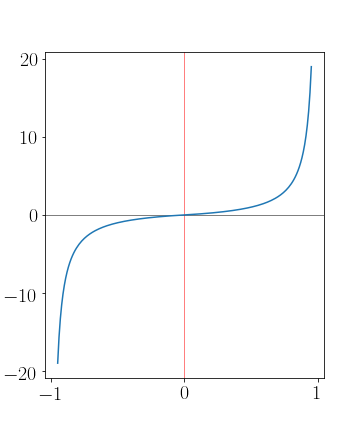
\includegraphics[scale=0.5]{interval.png}
\end{center}

Таким образом, композиция $h(g(f(x)))$ биективно переводит $[0;1)$ в $\R$. 
Следовательно, множество вещественных чисел имеет мощность континуума.

\subsection*{Эквивалентные последовательности}

\item Наконец, рассмотрим еще один способ конструирования множества $\R$.
\item Обозначим за $Q$ множество всех фундаментальных последовательностей рациональных чисел. Напомним, что последовательность фундаментальная, если почти все ее члены лежат в сколь угодно малой окрестности. На множестве $Q$ введем отношение следующим образом:
$$
q\sim r\Leftrightarrow \lim_{n\to\infty}(q_n-r_n) = 0.
$$

Вспоминая аксиому непрерывности в форме \textbf{A3}, мы понимаем, что если $q\sim r$, то эти последовательности имеют одинаковый предел. Отсюда легко видеть, что отношение $\sim$ является отношением эквивалентности, а значит, мы можем разбить $Q$ на классы эквивалентных последовательностей, т.е. построить фактормножество $R=Q/\sim$.

Вот это множество мы и объявляем множеством действительных чисел.

\item После чего мы должны ввести соответствующие операции и отношение сравнения.
\item Сложение классов эквивалентности вводится почленно:
$$
[q]+[r] = [q+r].
$$
Необходимо лишь доказать, что если $q\sim q'$ и $r\sim r'$, то $q+r\sim q'+r'$. Это легко заметить из следующего неравенства
$$
|(q+r)_n-(q'+r')_n| \le |q_n-q'_n| + |r_n-r'_n|,
$$
посколку два модуля справа стремятся к нулю.
\item Аналогично вводится умножение:
$$
[q]\cdot[r] = [qr]
$$
Для доказательства корректности определения заметим, что если $q\sim q'$ и $r\sim r'$, то
$$
|q_nr_n-q'_nr'_n| \le |q_n||r_n-r'_n| + |r'_n||q_n-q'_n|.
$$
Здесь справа стоят слагаемые, в каждом из которых ограниченная величина (в силу фундаментальности) умножается на величину, стремящуюся к нулю. Так что и все вместе стремится к нулю.
\item Наконец, о сравнении:
$$
[q]<[r], \mbox{ если }\exists\ep>0\;\exists N\;(\forall n>N) (q_n<r_n-\ep),
$$
т.е. для почти всех индексов разность $r_n-q_n$ отделена от нуля положительным числом $\ep$ (оно может быть очень маленьким, но не нулевым).
\item Итак, мы видим, что при определении $\R$ через эквивалентные классы фундаментальных последовательностей и операции, и отншение чисел просто переносятся один-в-один с рациональных чисел. Главная задача тут --- показать корректносьт такого определения. Кроме того, здесь мы активно пользуемся понятием предела.
\item Выше мы рассмотрели три модели $\R$:
\begin{enumerate}[M1]
\item Модель дедеиндовых сечений.
\item Модель двоичных (в общем случае $d$-ичных) дробей.
\item Модель классов фундаментальных последовательностей.
\end{enumerate}
\item Попутно мы установили раномощность $\R$ и множества всех подмножеств $\N$.

\item Возникает вопрос: если $\R$ такое большое множество, а $\Q$ такое маленькое (по мощности), есть ли какие-то множества, имеющие промежуточные мощности между счетной и континуумом? Ответ на этот вопрос дали два человека: К.Гёдель и П.Коэн. Первый доказал, что отсутствие промежуточных мощностей не противоречит аксиоматике теории множеств, второй --- что существование таких мощностей также не противоерчит аксиоматике теории множеств. Таким образом, мы оказываемся в ситуации пятого постулата Евклида, когда можем принимать или отвергать континуум-гипотезу\index{Континуум-гипотеза} (именно так называется утверждение о том, что между счетной мощностью и континуумом нет промежуточных мощностей), не опасаясь получить противоречие.
\end{enumerate}



\begin{comment}

19-20
2015_10_28 - 19-я и 20-я лекция д. ф.-м.н. А. В. Савватеева ч. ⅛
https://www.youtube.com/watch?v=m_N1Jc3HapU

2-30 соизмеримость отрезков
4-00 алгебраическая запись а=md b=nd
6-50 соотношение отрезков - рациональное число ⇔ соизмеримость

2015_10_28 - 19-я и 20-я лекция д. ф.-м.н. А. В. Савватеева ч. 2/8
https://www.youtube.com/watch?v=PsAxdahrv1Q

0-00 что если а и в несоизмеримы?
1-20 задача про кузнечика
2-50 ах+ву=с, а=корень из двух, в=1, сложное множество
6-00 если соизмеримы, то…
9-00 d(НОД(mn)z)

2015_10_28 - 19-я и 20-я лекция д. ф.-м.н. А. В. Савватеева ч. ⅜
https://www.youtube.com/watch?v=po68il5wqp0

1-30 все кратные отрезка d*НОД(mn)

2015_10_28 - 19-я и 20-я лекция д. ф.-м.н. А. В. Савватеева ч. 4/8
https://www.youtube.com/watch?v=9z8reMyp8ls

0-00 НОД (17 12)
2-00 геометрическая иллюстрация 17 на 12

2015_10_28 - 19-я и 20-я лекция д. ф.-м.н. А. В. Савватеева ч. ⅝
https://www.youtube.com/watch?v=Wi4R9Y-0XsI

0-00 геометрический алгоритм Евклида

2015_10_28 - 19-я и 20-я лекция д. ф.-м.н. А. В. Савватеева ч. 6/8
https://www.youtube.com/watch?v=vE6lFlpaVcE

0-00 цепные дроби 17/12
3-00 три ипостаси одного и того же
6-00 пишем любую цепную дробь

2015_10_28 - 19-я и 20-я лекция д. ф.-м.н. А. В. Савватеева ч. ⅞
https://www.youtube.com/watch?v=pHhQ_xoT1gA

Проверяем цепную дробь
Феномен цепных дробей - дроби с отличием на 1

2015_10_28 - 19-я и 20-я лекция д. ф.-м.н. А. В. Савватеева ч. 8/8
https://www.youtube.com/watch?v=xUPSD4zOPOM


0-00 ad-bc=+-1 GL2(Z)
2-00 кузнечик с соизмеримыми отрезками
3-00 геометрическое представление
7-00 "... словами и так до бесконечности!"


93-94
https://www.youtube.com/watch?v=1GAIDF8TPYQ

95-96
сечения Дедекинда и другие модели вещественных чисел
https://www.youtube.com/watch?v=eFIWK1NVJcA
56-00 о корнях, существует ли?
1-00-00 теорема: корни корней корней... стремится к 1
1-10-00 о степенях
1-10-30 n^k/f^n=>0
1-15-00 зажимание последовательности двумя другими
1-16-30 a^n/n!
\end{comment}



\section{Комплексные числа}

\subsection*{Конспект}
\begin{enumerate}\setlength{\itemsep}{1pt}
\item 
\item 
\item 
\item 
\item 
\item 
\item 
\item 
\item 
\item 
\end{enumerate}
\subsection*{Задачи}



\section{Гомотетии прямой и плоскости}

\subsection*{Конспект}
\begin{enumerate}\setlength{\itemsep}{1pt}
\item 
\item 
\item 
\item 
\item 
\item 
\item 
\item 
\item 
\item 
\end{enumerate}
\subsection*{Задачи}

